\documentclass[a4paper,11pt]{article}
\usepackage{./jheppub}
%\setcounter{secnumdepth}{3}
% Useful packages
\usepackage{tikz-cd}
\usepackage{amsmath}
\usepackage{array,booktabs}
\usepackage{hyperref}
%%\usepackage{showlabels}
\usepackage{amsthm}
\newtheorem{theorem}{Theorem}
\newtheorem{lemma}[theorem]{Lemma}
\newtheorem{corollary}[theorem]{Corollary}
\newtheorem{proposition}[theorem]{Proposition}
\theoremstyle{definition}
\newtheorem{definition}{Definition}[section]
\newtheorem{prop}{Conjecture}
\newtheorem{cor}{Corollary}
%-------------------packages-------------------------
\usepackage{enumerate}
\usepackage[utf8]{inputenc}
\usepackage{amssymb,amsbsy,mathtools,amsmath}
\usepackage{braket}
\usepackage{graphicx}
\usepackage{xcolor}
%\usepackage{multirow}
\usepackage{hyperref}
%\usepackage{caption}
%\usepackage{subcaption}
%\mathcal{A}ptionsetup{compatibility=false}
\usepackage{natbib}
%\usepackage{dcolumn}% Align table columns on decimal point
\usepackage{bm}% bold math
\usepackage{soul}
%\usepackage{showlabels}
%\newtheorem{proposition}{Proposition}
\newcommand{\E}{\mathbb{E}}
\newcommand{\dd}{\,\mathrm{d}}
%\newcommand{\mathcal{A}}{\mathcal{A}}
\newcommand{\cH}{\mathcal{H}}
\newcommand{\KLL}{D_{\mathrm{KL}}}
\newcommand{\Mop}{\mathsf{M}}

%Includes "References" in the table of contents
\usepackage[nottoc]{tocbibind}

\usepackage{bbm}
\usepackage{amsthm}
%\newtheorem{theorem}{Theorem}
%\newtheorem{lemma}[theorem]{Lemma}
%\newtheorem{corollary}[theorem]{Corollary}
%\theoremstyle{definition}
%\newtheorem{definition}{Definition}[section]
\usepackage{amssymb}
\newcommand{\id}{\mathbb{I}}
\newcommand{\Tr}{\text{Tr}}
\newcommand{\Div}{\operatorname{div}}
\usepackage{amsmath}
%\usepackage{tikz}
\usepackage{braket}
%\usepackage{quantikz}
\usepackage{graphicx}
\usepackage{caption}
\newcommand{\mA}{\mathcal{A}}
\newcommand{\mB}{\mathcal{B}}
\newcommand{\mP}{\mathcal{P}}
\newcommand{\mR}{\mathcal{R}}
\newcommand{\nn}{\nonumber}
\newcommand{\mL}{\mathcal{L}}
\newcommand{\lb}{\left(}
\newcommand{\rb}{\right)}
\newcommand{\mH}{\mathcal{H}}
\usepackage{subcaption}
\newcommand{\tOO}{\tilde{\mathcal{O}}}
\newcommand{\mO}{\mathcal{O}}
\newcommand{\mK}{\mathcal{K}}
\newcommand{\ep}{\epsilon}
\newcommand{\mbR}{\mathbb{R}}
\newcommand{\mM}{\mathcal{M}}
\newcommand{\mT}{\mathcal{T}}
\newcommand{\NL}[1]{\textcolor{blue}{#1}}
\newcommand{\p}{\partial}
\newcommand{\tr}{\text{tr}}
\newcommand{\tT}{\tilde{T}}
\newcommand{\Ad}{\operatorname{Ad}}
\newcommand{\Dom}{\operatorname{Dom}}
\newcommand{\mE}{\mathcal{E}}
\newcommand{\relcomm}[2]{#1'\cap #2}

\newcommand{\SO}[1]{\textcolor{purple}{#1}}
%\newcommand{\MM}[1]{\textcolor{red}{#1}}
\newcommand{\KL}[1]{\textcolor{brown}{#1}}
\newcommand{\YC}[1]{\textcolor{teal}{#1}}
\newcommand{\cL}{\mathcal{L}}
\setlength{\emergencystretch}{2em}
\begin{document}

\title{Subsystem flow in QFT and holography}

\author{Yidong Chen$^1$,}
\affiliation{$^1$Department of Mathematics, University of Illinois at Urbana-Champaign, Illinois, IL 61801, USA}
\author{Nima Lashkari$^2$,}
\author{Kwing Lam Leung$^2$}
\affiliation{$^2$Department of Physics and Astronomy, Purdue University, West Lafayette, IN 47907, USA}
\emailAdd{yidongc2@illinois.edu}
\emailAdd{nima@purdue.edu}
\emailAdd{leung60@purdue.edu}

\abstract{When the modular flow of a subregion of a quantum field theory is not geometric, how is its departure from the geometric flow of a larger region computed and controlled? We answer this for the \emph{subsystem flow} $D_{B\subset A}(z)=\Delta_A^{-iz}\Delta_B^{iz}$ of an inclusion of local algebras with a common cyclic and separating vacuum. For wedges translated by any vector in the closed wedge, the subsystem flow is an exact translation, $D(z)=\exp i[\,b_+(e^{2\pi z}-1)P_+-b_-(e^{-2\pi z}-1)P_-]$, contractive precisely on Borchers' strip, with the half-sided modular inclusion as the null boundary case; its two-dimensional CFT matrix elements factorize into two chiral factors, each amplified in one direction of modular time, which makes the modular Lyapunov rate $2\pi$ and its scrambling window explicit. Double cones in CFT give fractional-linear flows with the same analytic structure, and a massive free scalar gives a nonconformal example with logarithmic null singularities. Beyond geometric examples we derive the first-order correction of double-cone flows in regulated conformal perturbation theory and establish nonperturbative large-region estimates: a uniform, time-averaged bound on localized vectors after a cutoff in boost energy, a strong limit on fixed vectors, and, in CFT, a pointwise bound with explicit rate $e^{-2\pi s}$ on vectors of finite conformal energy, which shows that the boost-energy cutoff is the price of uniformity over an entire local algebra. Finally, the subsystem flow at imaginary modular time $i/4$ is the $L^2$-nuclearity operator of Buchholz, D'Antoni and Longo; we compute it exactly for wedge inclusions, where it is the Gibbs operator of the displacement Hamiltonian $b^1P_0+b^0P_1$, and for concentric double cones, where it is unitarily equivalent to $(r/R)^{2L_0}$ and the nuclearity index is the vacuum character at $q=r/R$.}

\maketitle

%\tableofcontents

\section{Introduction}\label{sec:intro}

Modular theory assigns a distinguished evolution to a state and an algebra of observables. In the vacuum of a relativistic QFT, wedge modular flow is a Lorentz boost under the Bisognano--Wichmann hypothesis~\cite{bisognanowichmann}. For a double cone in a CFT, conformal symmetry gives a geometric modular flow~\cite{HislopLongo1982}. General subregions have no such known spacetime action. The question addressed in this paper is how the departure of a subregion's modular flow from the geometric flow of a larger region is computed when both are geometric, how it is controlled when the smaller one is not, and what spectral information it carries.

The object that organizes the answer is the \emph{subsystem flow} of an inclusion $\mathcal A(B)\subset\mathcal A(A)$ with vacuum modular operators $\Delta_B$ and $\Delta_A$,
\begin{equation}
 D_{B\subset A}(z)=\Delta_A^{-iz}\Delta_B^{iz}.
 \label{eq:intro-D}
\end{equation}\KL{(I think calling it outer/inner flow/evolution may cause confusion, sounds like it is related to outer/inner automorphism.)}
For real $z$ this first reverses the intrinsic modular evolution of $B$ and then applies the physical modular evolution of $A$; its adjoint action transports the retained algebra along the outer flow. Borchers' characterization of inclusions gives a bounded analytic continuation to $0<\operatorname{Im}z<1/2$~\cite{revolutionizing}. The operator is in general a cocycle rather than a one-parameter group, and its infinitesimal generator does not determine its finite-time action. In the algebraic literature it is known as the characteristic function of the inclusion; the companion paper~\cite{companion} develops it as an object of ergodic theory and error correction, and we use its name and conventions here.

\paragraph{Main results:}
The paper has four parts, which answer the question above at increasing levels of generality.

\emph{Geometric inclusions} (Section~\ref{sec:geometric-subregion-flows}): When both flows are geometric their composition is exact. For a wedge translated by any vector $b$ in the closed wedge, with null components $b_\pm\ge0$ and null momenta $P_\pm\ge0$, we have (Theorem~\ref{thm:wedge-characteristic})
\begin{equation}
 D_{W(b)\subset W(0)}(z)=\exp\Big\{i\big[\,b_+(e^{2\pi z}-1)P_+-b_-(e^{-2\pi z}-1)P_-\big]\Big\}.
 \label{eq:intro-wedge}
\end{equation}
The generator is manifestly positive, the contraction strip is exactly Borchers' strip, the half-sided modular inclusion is the null boundary case $b_-=0$, and the finite-time displacement traces a timelike curve rather than a one-parameter group. In two-dimensional CFTs the matrix elements factorize into two chiral factors, each amplified in one direction of modular time (Proposition~\ref{prop:wedge-factorized}); this makes the modular Lyapunov exponent $2\pi$ and its scrambling window $t_*=\tfrac1{2\pi}\log(1/\epsilon)$ explicit (Section~\ref{subsec:small-deformations}). Double cones in CFT give fractional-linear flows with the same analytic structure, and a massive free scalar gives a nonconformal example with logarithmic null singularities. The universal analytic strip bounds the growth of normalized matrix elements (Lemma~\ref{lem:strict-modular-chaos-bound}); the geometric examples approach the bound in a controlled window without saturating it.

\emph{Conformal perturbation theory} (Section~\ref{section:conformalperturbation}): Perturbing a CFT by a relevant scalar, the logarithmic variation of the reduced state expresses the leading modular correction as an integral along the unperturbed modular orbit. We identify the local and nonlocal contributions, include the variation of the vacuum, and obtain a regulated first-order formula for the matrix elements. For wedge inclusions the flow term vanishes identically, which isolates what is new for double cones.

\emph{Nonperturbative large-region estimates} (Section~\ref{section:approx}): Fredenhagen's estimate controls modular evolution when a localized observable remains inside the smaller region for a long interval of outer modular time~\cite{fredenhagen}. For double cones exhausting a wedge this gives a uniform, time-averaged bound on localized vectors after a cutoff in boost energy (Theorem~\ref{theorem:mainresult}), while modular convergence gives the uncut limit on every fixed vector (Theorem~\ref{theorem:ballinsideball}). We explain why the cutoff is needed and show that it can be traded for a physical assumption: in a CFT the difference of subsystem flows is bounded pointwise in modular time by $(e^{2\pi|t|}-1)/(2e^{2\pi s}R_0)$ times the conformal energy of the vector (Theorem~\ref{thm:CFT-pointwise}), with no cutoff and no averaging. The growth $e^{2\pi|t|}$ of this bound is exactly the breakdown of the approximation at the Fredenhagen time $|t|\approx s$.

\emph{Nuclearity and the spectrum of an inclusion} (Section~\ref{sec:nuclearity}): The subsystem flow at imaginary modular time $i/4$ is the operator whose trace-class property is the $L^2$-nuclearity of Buchholz, D'Antoni and Longo~\cite{BDL2007}. For wedge inclusions it is $e^{-(b^1P_0+b^0P_1)}U(-b)$, the Gibbs operator of the displacement Hamiltonian composed with a translation, and its square is $e^{-(K_A-K_B)/\pi}$ (Proposition~\ref{prop:wedge-nuclearity}); for a spacelike displacement $a$ this is $e^{-2aP_0}$, which connects modular nuclearity to the energy nuclearity of Buchholz and Wichmann. For concentric double cones in CFT the operator is a complexified M\"obius element, and $D(i/4)^*D(i/4)$ is unitarily equivalent to $(r/R)^{2L_0}$, so that the nuclearity index is the vacuum character $\operatorname{Tr}(r/R)^{L_0}$ (Proposition~\ref{prop:cone-nuclearity}). The modular Hamiltonian of an inclusion introduced in the companion paper is thus $2(b_+P_++b_-P_-)$ for wedges and $2\log(R/r)L_0$ for cones.

Throughout, Theorem~\ref{thm:wedge-characteristic}, Section~\ref{section:approx}, and Proposition~\ref{prop:wedge-nuclearity} hold in any dimension; all explicit matrix elements, Section~\ref{subsec:ball-inside-wedge}, Section~\ref{section:conformalperturbation}, and Proposition~\ref{prop:cone-nuclearity} are in $1+1$ dimensions. Section~\ref{sec:setup} collects the modular setup, the interpretation of the matrix elements as reflected two-point functions, and the growth bound, so that the later sections can be read independently of the companion paper. The appendices give the increasing-region geometry, the modular convergence argument, and the distributional kernel identities.


\section{Subsystem flows in QFT}\label{sec:qft-subtheories}

\NL{AI written}

Before computing the subsystem flow of nested local regions, it is
useful to distinguish an inclusion transported by modular dynamics from
a subalgebra on which that dynamics closes. The latter possibility is
quite restrictive for local algebras in the vacuum, but it arises
naturally from internal or spacetime symmetries. It is also the starting
point of Borchers' theory of modular-covariant subalgebras and tensor
product decompositions of QFT~\cite{revolutionizing}. We review these
structures here, emphasizing the difference between autonomy for a
single region and a coherent relativistic subtheory, and then apply
them to balls, disconnected regions and generalized symmetries.

\subsection{Modular-covariant subalgebras and the subsystem comparison}
\label{subsec:qft-modular-covariant}
Let $\mathcal M=\mathcal A(O)$ be the local algebra of a region $O$,
with vacuum state $\omega(x)=\langle\Omega,x\Omega\rangle$ and modular
automorphisms $\sigma_t^{\omega;M}=\operatorname{Ad}\Delta_M^{it}$.
Following Borchers, a unital von Neumann subalgebra
$\mathcal N\subset\mathcal M$ is \emph{modular covariant} when
\begin{equation}
 \sigma_t^{\omega;M}(\mathcal N)=\mathcal N,
 \qquad t\in\mathbb R .
 \label{eq:qft-modular-covariant}
\end{equation}
This condition means that the retained observables form an autonomous
subsystem of modular dynamics; individual elements of $\mathcal N$ need
not be fixed. For a faithful normal reference state, Takesaki's theorem
identifies Eq.~\eqref{eq:qft-modular-covariant} with the existence of a
unique normal conditional expectation
\begin{align}
 \mathcal E_\omega:\mathcal M\longrightarrow\mathcal N,
 \qquad \omega\circ\mathcal E_\omega=\omega,
 \qquad
 \mathcal E_\omega\circ\sigma_t^{\omega;M}
   =\sigma_t^{\omega;M}\circ\mathcal E_\omega .
 \label{eq:qft-Takesaki-expectation}
\end{align}
Thus modular autonomy supplies an exact coarse-graining compatible
with the reference vacuum. In the companion paper it is interpreted as
a correctable restriction channel for the family of states extending
from $\mathcal N$ through $\mathcal E_\omega$~\cite{companion}.

Let $\mathcal H_N=\overline{\mathcal N\Omega}$ and let
$e_N=[\mathcal N\Omega]$ project onto this subspace. Borchers'
Lemma VI.1.2 and Takesaki's theorem give, when $\mathcal N$ is modular
covariant,
\begin{align}
 [e_N,\Delta_M^{it}]=[e_N,J_M]=0,
 \qquad
 e_Nxe_N=\mathcal E_\omega(x)e_N,
 \quad x\in\mathcal M,
 \label{eq:qft-Jones-compression}
\end{align}
and $\Delta_M^{it}|_{\mathcal H_N}$ is the modular group of
$(\mathcal N|_{\mathcal H_N},\Omega)$. The Jones projection $e_N$
belongs to the GNS Hilbert-space description and is not in general a
projection of the local observable algebra. It characterizes the
modular-covariant algebra by
$\mathcal N=\mathcal M\cap\{e_N\}'$.

For such an inclusion, the compressed comparison
\begin{equation}
 C_{N\subset M}(t)
  =V^*\Delta_M^{-it}V\Delta_N^{it}=1_{\mathcal H_N},
 \qquad V:\mathcal H_N\hookrightarrow\mathcal H,
 \label{eq:qft-compressed-autonomy}
\end{equation}
is trivial. This is to be distinguished from the unitary subsystem
flow of a \emph{common-cyclic} inclusion,
\begin{equation}
 D_{B\subset A}(t)=\Delta_A^{-it}\Delta_B^{it},
 \qquad \mathcal A(B)\subset\mathcal A(A),
 \label{eq:qft-comparison-reminder}
\end{equation}
which is the object studied below. In particular, modular-covariant
proper subalgebras generally have a noncyclic vacuum on the ambient
Hilbert space, while local inclusions in the vacuum have a common cyclic
vector by Reeh--Schlieder.

Indeed, if $\Omega$ is cyclic for $\mathcal N$ and separating for
$\mathcal M$, an $\omega$-preserving expectation must be the identity:
for $n\in\mathcal N$ and $x\in\mathcal M$,
\begin{align}
 \langle n\Omega,(x-\mathcal E_\omega(x))\Omega\rangle
 &=\omega\!\left(n^*x-n^*\mathcal E_\omega(x)\right)=0 .
\end{align}
Cyclicity gives $(x-\mathcal E_\omega(x))\Omega=0$ and separatingness
then gives $x=\mathcal E_\omega(x)$. Therefore
\begin{equation}
\ \Omega\text{ cyclic for }\mathcal N,
 \ \Omega\text{ separating for }\mathcal M,
 \ \mathcal N\subsetneq\mathcal M
 \ \Longrightarrow\
 \sigma_t^{\omega;M}(\mathcal N)\neq\mathcal N
 \text{ for some }t.\ 
 \label{eq:qft-cyclic-no-go}
\end{equation}
The modular history of $\mathcal N$ then generates the entire ambient
algebra:
\begin{equation}
 \left(\bigcup_{t\in\mathbb R}\sigma_t^{\omega;M}(\mathcal N)
 \right)''=\mathcal M.
 \label{eq:qft-cyclic-generation}
\end{equation}
To prove Eq.~\eqref{eq:qft-cyclic-generation}, apply the same argument
to the modular-invariant algebra generated by the orbit; it is still
cyclic on $\Omega$. This generating property requires neither mixing
nor a nuclearity condition. Conversely, a compact-symmetry fixed-point
algebra can be proper and modular covariant precisely because its
vacuum need not be cyclic on the full representation space.

\subsection{Coherence, tensor factors and hidden charges}
\label{subsec:qft-coherent-subtheories}
Modular covariance for a single algebra is weaker than having a local
subtheory. In Section VI.3 of Ref.~\cite{revolutionizing}, Borchers
considers subalgebras $\mathcal N(W)\subset\mathcal M(W)$ for wedges,
and $\mathcal N(D)\subset\mathcal M(D)$ for double cones, and requires a
\emph{coherent} family: the projections
$e_O=[\mathcal N(O)\Omega]$ agree for all regions in the family,
$e_O=e$. Under the hypotheses used there, including the
Bisognano--Wichmann property and a suitable wedge-intersection
construction, this common subspace $e\mathcal H$ is invariant under
Poincar\'e transformations, and restriction of the local algebras to
$e\mathcal H$ defines a covariant QFT. Thus one may have a proper
modular-covariant algebra for one region without a coherent net
representing an independent relativistic theory.

For a modular-covariant factor $\mathcal N\subset\mathcal M$, its
relative commutant $\mathcal R=\mathcal N'\cap\mathcal M$ is also
modular covariant. A theorem quoted in Section VI.4 of
Ref.~\cite{revolutionizing} states that
\begin{align}
 \mathcal N\vee\mathcal R&\simeq
      \mathcal N\,\bar\otimes\,\mathcal R,
 &\omega(nr)&=\omega(n)\omega(r),
 \quad n\in\mathcal N,\ r\in\mathcal R .
 \label{eq:qft-Borchers-product}
\end{align}
If $\mathcal N\vee\mathcal R=\mathcal M$, the modular-covariant algebra
identifies a tensor-factor decomposition. The alternative
$\mathcal R=\mathbb C1$ for a proper inclusion is the \emph{hidden charge}
case: charged fields can extend the smaller theory without producing a
commuting tensor factor. More generally,
$\mathcal N\vee\mathcal R\subsetneq\mathcal M$ allows both an independent
component and additional charged sectors. The coherent-net assumption
is crucial when interpreting these local statements as decompositions
of an entire QFT.

\subsection{Rotation symmetry and angular harmonics of a ball}
\label{subsec:qft-ball-rotations}
Consider a ball $B_R$ centered at the spatial origin in a relativistic
vacuum QFT in spacetime dimension $d=3$ or $4$. Its spatial rotation
group is $G=SO(d-1)$. Rotations preserve the double cone $D(B_R)$ and
the vacuum,
\begin{equation}
 U(g)\mathcal A(B_R)U(g)^*=\mathcal A(B_R),
 \qquad U(g)\Omega=\Omega .
\end{equation}
Consequently modular uniqueness implies
\begin{gather}
 [U(g),\Delta_{B_R}^{it}]=0,\nonumber\\
 \mathcal N_{\mathrm{rot}}(B_R)
  :=\mathcal A(B_R)^G, \qquad
 \sigma_t^{B_R}(\mathcal N_{\mathrm{rot}}(B_R))
   =\mathcal N_{\mathrm{rot}}(B_R).
 \label{eq:qft-rotation-invariant-algebra}
\end{gather}
The Haar expectation $\int_G\dd g\,\operatorname{Ad}U(g)$ is vacuum
preserving. This result is \emph{independent} of whether the modular
Hamiltonian is geometric; it applies equally to massive and
interacting vacuum QFTs.

For a CFT the stronger geometrical statement follows from the
conformal Killing vector and the formal one-sided modular Hamiltonian,
\begin{align}
 k_{B_R}&=2\pi\int_{|\mathbf x|<R}\!\dd^{d-1}x\,
 \frac{R^2-r^2}{2R}\,T_{00}(0,\mathbf x)+\text{const.},\nonumber\\
 \xi_B&=\frac{\pi}{R}\big[(R^2-t^2-r^2)\partial_t
                         -2tr\partial_r\big].
 \label{eq:qft-ball-geometric-modular}
\end{align}
Here $k_{B_R}$ is the one-sided generator $-\log\rho_{B_R}$ in a
regulated description; it must not be confused with the full modular
operator $K_{B_R}=-\log\Delta_{B_R}$ acting on the vacuum Hilbert
space. Both induce the same automorphisms on the ball algebra.
Up to the convention for the direction of modular time, $\xi_B$
generates the modular action. Because it has no angular component, the
angular wave functions of a scalar primary do not mix. In $2+1$
dimensions,
\begin{align}
 \mathcal O_m(t,r)&=\int_0^{2\pi}\!\frac{\dd\theta}{2\pi}
  e^{-im\theta}\mathcal O(t,r,\theta),
 &\sigma_s^{B_R}(\mathcal O_m)&\text{ has angular momentum }m,
 \quad m\in\mathbb Z .
 \label{eq:qft-harmonics-3d}
\end{align}
In $3+1$ dimensions the analogous modes are
\begin{align}
 \mathcal O_{\ell m}(t,r)&=\int_{S^2}\!\dd\Omega\,
    Y_{\ell m}(\Omega)^*\mathcal O(t,r,\Omega),
 &\sigma_s^{B_R}(\mathcal O_{\ell m})
   &\text{ has the same }(\ell,m),
 \label{eq:qft-harmonics-4d}
\end{align}
with the usual interpretation as smeared operator-valued
distributions. In a CFT, scalar-primary modes of the \emph{same field}
retain these labels under the geometrical flow; a conformal Jacobian
depending on $t,r$ multiplies the transformed field. In a general QFT,
only the representation-theoretic statement survives: the full
isotypic operator space of given angular momentum is preserved, but
modular evolution can mix different fields and composite operators
with the same total angular momentum.

A nonzero-angular-momentum space is not normally an algebra. In
$2+1$ dimensions, if
\begin{equation}
 \mathcal M_m=\{x\in\mathcal M:
 U(\theta)xU(\theta)^*=e^{im\theta}x\},
\end{equation}
then $\mathcal M_m\mathcal M_n\subset\mathcal M_{m+n}$ and
$\mathcal M_m^*=\mathcal M_{-m}$. In $3+1$ dimensions products combine
according to the Clebsch--Gordan rules. Algebras generated by complete
rotational multiplets are modular covariant, but need not be proper;
the rotational singlets themselves form the canonical fixed-point
algebra. For a free massive or massless scalar, Gaussian factorization
makes the radial harmonic algebras separately invariant, even without
geometric ball modular flow.

This is not automatically a coherent relativistic subtheory. The
projection onto the singlet Hilbert space for rotations about the
origin is $e_0=\int_G\dd g\,U(g)$. For a translated ball centered at
$a$, the corresponding projection is
$e_a=U(a)e_0U(a)^*$, generically different from $e_0$.
The rotation-invariant algebras are autonomous for \emph{each fixed
ball}, but their cyclic-subspace projections do not generally agree
under translations. This contrasts with an unbroken compact internal
zero-form symmetry: its group-averaging projection $P_G$ is independent
of the region and commutes with the Poincar\'e representation, giving
a coherent neutral subtheory.

\subsection{Disconnected regions and generalized symmetries}
\label{subsec:qft-generalized-symmetries}
For an unbroken internal zero-form symmetry on two spacelike-separated
regions, let
$\mathcal M=\mathcal F(O_1)\vee\mathcal F(O_2)$.
The \emph{diagonal} symmetry preserves the vacuum and hence
$\mathcal M^G$ is modular covariant. Importantly, it may contain
bilocal neutral charge--anticharge intertwiners,
$\psi_q(O_1)\psi_{-q}(O_2)$, which are not generated by
$\mathcal F(O_1)^G\vee\mathcal F(O_2)^G$.
Independent symmetry rotations of the two components are not generally
vacuum preserving, because the vacuum is correlated across components.
Thus the globally neutral algebra is the natural modular-invariant
choice; componentwise neutrality is a different coarse-graining.

For a one-form symmetry in $2+1$ dimensions~\cite{GaiottoKapustinSeibergWillett2015}, take instead an annular
spatial region $A$. Its nontrivial first homology allows Wilson or
disorder operators not additively generated in arbitrarily small
contractible regions. For incomplete observable nets one can have
\begin{equation}
 \mathcal N=\mathcal A_{\mathrm{add}}(A)
 \subsetneq\mathcal M=\mathcal A_{\mathrm{max}}(A)
 :=\mathcal A_{\mathrm{add}}(A')'.
 \label{eq:qft-additive-maximal}
\end{equation}
The maximal algebra is defined relative to the chosen representation
and causal complement. The extra winding sectors may admit a
crossed-product-type description and a conditional expectation that
removes them~\cite{GaiottoKapustinSeibergWillett2015,CasiniHuertaMaganPontello2021,CasiniMagan2021}.
But one should not identify that expectation with vacuum-preserving
Haar averaging: in the vacuum, Reeh--Schlieder makes $\Omega$ cyclic
for $\mathcal N$ and (when the complement is nonempty) separating
for $\mathcal M$. Equation~\eqref{eq:qft-cyclic-no-go} therefore gives
\begin{align}
 \sigma_t^{\omega;\mathcal M}(\mathcal N)&\neq\mathcal N
 \quad\text{for some }t,\nonumber\\
 \bigvee_{t\in\mathbb R}
 \sigma_t^{\omega;\mathcal M}(\mathcal N)&=\mathcal M .
 \label{eq:qft-annulus-generation}
\end{align}
The additive algebra is not autonomous under the maximal algebra's
modular flow, even though its modular orbit generates all the
non-additive sectors. Compactness of a dual action does not remove this
obstruction: a nontrivial action fixing $\mathcal N$ pointwise cannot
preserve $\omega$ if $\mathcal N\Omega$ is dense.

It is important here to distinguish a charged Wilson loop from a
topological generator of the one-form symmetry. For example, $W_q(C)=\exp(iq\oint_C a)$ in Maxwell theory is not
a topological operator, and a contractible loop generally probes field
strength fluctuations and excites the vacuum. In contrast, an
appropriately normalized topological one-form symmetry generator may
be deformable through an empty disk. The loop $C$ can be
noncontractible in the annulus but contractible in a larger ball, where
$W_q(C)$ may become additive without becoming trivial.
Likewise, an annular twist rotating the winding sectors is not
necessarily the restriction of a global vacuum-preserving symmetry
action. These distinctions reconcile the modular non-invariance of
Eq.~\eqref{eq:qft-annulus-generation} with the existence of genuine
unbroken generalized symmetries.

\paragraph{Implications for subsystem flows.} 
The two opposite regimes can now be summarized without identifying
their modular operators. For a symmetry-fixed algebra
$\mathcal N\subset\mathcal M$ with an invariant reference state, its
compressed comparison is trivial,
$C_{N\subset M}(t)=1$ on $\overline{\mathcal N\Omega}$.
For nested local algebras with a common cyclic and separating vacuum,
the unitary comparison~\eqref{eq:qft-comparison-reminder} need not be
trivial: its adjoint action transports the inner algebra according to
\begin{equation}
 \operatorname{Ad}D_{B\subset A}(t)(\mathcal A(B))
   =\sigma_{-t}^{A}(\mathcal A(B)).
 \label{eq:qft-subsystem-transport}
\end{equation}
Under a strict local inclusion the right-hand side cannot equal
$\mathcal A(B)$ for all $t$. The following sections compute and bound
this failure of closure in geometric and nongeometric examples. In this
sense the subsystem flow measures how far a local inclusion lies from
a vacuum-preserving, exactly recoverable subtheory, whereas compact
symmetry fixed points provide benchmarks at which the compressed
comparison vanishes.

\section{Modular setup and subsystem flows}\label{sec:setup}

\subsection{Vacuum modular dynamics}

Let $O\mapsto\mathcal A(O)$ be an isotonic local net in a vacuum Hilbert space $\mathcal H$. We assume that the normalized vacuum $\Omega$ is cyclic and separating for the wedge and double-cone algebras used below. The closure of the antilinear map $S_Ca\Omega=a^*\Omega$, $a\in\mathcal A(C)$, has polar decomposition $S_C=J_C\Delta_C^{1/2}$. The modular automorphism group is
\begin{equation}
 \sigma_C^t(a)=\Delta_C^{it}a\Delta_C^{-it},\qquad K_C=-\log\Delta_C.
 \label{eq:modular-flow}
\end{equation}
We call $\beta_C^t=\sigma_C^{-t}=\operatorname{Ad}\Delta_C^{-it}$ the physical modular flow. This convention gives the upper-strip KMS condition and fixes the orientation of the boosts below~\cite{revolutionizing,companion}. The full $K_C$ acts on the vacuum Hilbert space and annihilates $\Omega$. When a regulated density matrix is used, its one-sided modular Hamiltonian $k_C=-\log\rho_C$ has the same adjoint action on $\mathcal A(C)$, but is a different operator.

For $B\subset A$, the common vacuum puts both modular operators on $\mathcal H$. The Tomita map of $A$ extends that of $B$, $S_Ab\Omega=b^*\Omega=S_Bb\Omega$ for $b\in\mathcal A(B)$, giving $\Delta_A\le\Delta_B$ as closed quadratic forms. Borchers' characteristic-function theorem gives the following continuation~\cite{revolutionizing}.

\begin{theorem}[Borchers; the characteristic strip]\label{prop:strip}
The real-time operator \eqref{eq:intro-D} extends analytically to $0<\operatorname{Im}z<1/2$, with $\|D_{B\subset A}(z)\|\le1$ on the closed strip. Its values on both boundary lines are unitary and strongly continuous, and $D(i/2)=J_AJ_B$. The operator preserve the vacuum, i.e. $D(z)\Omega=\Omega$.
\end{theorem}

\subsection{Transport and infinitesimal comparison}
\KL{(I would suggest using $\text{Ad}_O$ instead of $\text{Ad}O$ for the adjoint action)}
For $b\in\mathcal A(B)$ and real $t$,
\begin{equation}
 \operatorname{Ad}D_{B\subset A}(t)(b)=\sigma_A^{-t}\bigl(\sigma_B^t(b)\bigr),
 \qquad
 \operatorname{Ad}D_{B\subset A}(t)(\mathcal A(B))=\sigma_A^{-t}(\mathcal A(B)).
 \label{eq:transport}
\end{equation}
Thus the inner evolution removes motion already intrinsic to the subsystem, while the outer evolution follows its embedding in the larger algebra. No conditional expectation is assumed, and $D(t)$ need not be an element of either local algebra. It satisfies the cocycle identity
\begin{equation}
 D(t+s)=\Delta_A^{-it}D(s)\Delta_A^{it}D(t).
 \label{eq:cocycle}
\end{equation}
On vectors in the common operator domain of $K_A$ and $K_B$,
\begin{equation}
 -i\,\partial_tD(t)\psi\big|_{t=0}=(K_A-K_B)\psi .
 \label{eq:generator}
\end{equation}
\KL{(I think we should remove the following sentences. We never want to replace it by $e^{it(K_A-K_B)}$. For one parameter flow, the iff condition is $\Delta_A^{-it}\Delta_B^{is}\Delta_A^{+it} = \Delta_B^{is}$, which we could say better than this. Like if common cyclic separating, then the this won't happen because of uniquness of modular flow, etc.)}

This compares generators at the origin. \KL{The finite-time product retains their ordering, so replacing it by $e^{it(K_A-K_B)}$ requires an additional argument.} The geometric examples of Section~\ref{sec:geometric-subregion-flows} determine the finite-time action directly, \KL{and show that it is not a one-parameter group even when $K_A-K_B$ is a simple operator.} The generator is positive, $K_A-K_B\ge0$, because $\Delta_A\le\Delta_B$; its expectation value in a state is the sum of two relative-entropy differences, and vanishes exactly when a vacuum-preserving conditional expectation onto $\mathcal A(B)$ exists~\cite{companion}.

\subsection{Matrix elements as reflected two-point functions}\label{subsec:matrix-elements}

For vectors $|O_j\rangle=O_j\Omega$ with finite quarter-modular norms, define
\begin{equation}
 F(z)=\langle O_1|\Delta_A^{1/2}D_{B\subset A}(-z)|O_2\rangle,
 \qquad
 N=\|\Delta_A^{1/4}O_1\Omega\|\,\|\Delta_B^{1/4}O_2\Omega\|>0,
 \qquad
 f(z)=F(z)/N.
 \label{eq:F-def}
\end{equation}
\KL{(Geometric only for special cases, I don't think we should describe it like this. We may say if there is Haag's duality, then it maps to the compliment region/spacelike separating region. Isn't it weird to define $O^J$ with the star? And should it be $O_1^{J*}$ or $O_1^{J}$ in the following equation)} The factor $\Delta_A^{1/2}$ has a geometric meaning. By Tomita's relation $\Delta_A^{1/2}O_1\Omega=J_AO_1^*\Omega=O_1^J\Omega$, where $O_1^J:=J_AO_1^*J_A\in\mathcal A(A)'$ is the \emph{reflected} operator; for a wedge, $J_A$ is the CPT-type reflection through the edge~\cite{bisognanowichmann}, so $O_1^J$ is the same field at the reflected point in the opposite wedge, with any internal conjugation included. Using $\Delta^{it}\Omega=\Omega$ for both algebras, for real $t$,
\begin{equation}
 F(t)=\big\langle\Omega\big|\,\beta_A^t\!\bigl(O_1^{J*}\bigr)\;\beta_B^t\!\bigl(O_2\bigr)\big|\Omega\big\rangle .
 \label{eq:F-reflected}
\end{equation}
The matrix element is therefore a two-point function in which the reflected outer insertion is transported by the outer physical flow and the inner insertion by the inner physical flow. When both flows are geometric this is a vacuum two-point function at geometrically determined points; when the inner flow is not geometric, \eqref{eq:F-reflected} is the quantity to be approximated. On the real axis the two insertions are spacelike separated, which is why no $i\epsilon$ prescription appears in the explicit formulas below.

The continuation to complex $z$ is understood through the bounded expression
\begin{equation}
 f(z)=\frac{\langle\Delta_A^{1/4}O_1\Omega|D_{B\subset A}(i/4-z)|\Delta_B^{1/4}O_2\Omega\rangle}{N}.
 \label{eq:f-continuation}
\end{equation}
Cauchy--Schwarz and Theorem~\ref{prop:strip} give $|f(z)|\le1$ for $|\operatorname{Im}z|\le1/4$. This centered strip is universal under the stated domain assumptions. A larger zero-free continuation, when it occurs for explicit point-field correlators, is a property of those correlators. The bare vacuum expectation $\langle\Omega|D(z)|\Omega\rangle=1$ contains no information about the inclusion; the excited insertions provide the matrix elements studied here.

\subsection{The growth bound on normalized matrix elements}\label{subsec:modular-chaos-bound}

The strip bound underlying modular chaos~\cite{deBoerLamprou2020} follows from \eqref{eq:f-continuation} alone, and we record it here before turning to examples. Write
\begin{equation}
 f(z)=\frac{\langle O_1|\Delta_A^{1/2+iz}\Delta_B^{-iz}|O_2\rangle}{N}=1+i\mathcal M(z).
 \label{eq:normalized-characteristic}
\end{equation}
The contraction property gives $|f(z)|\le1$ for $|\operatorname{Im}z|\le1/4$, with analytic interior and continuous boundary values. Hence
\begin{equation}
 \operatorname{Im}\mathcal M(z)=1-\operatorname{Re}f(z)\ge0 .
 \label{eq:positive-imaginary-part}
\end{equation}
The map $E=ie^{-2\pi z}$ sends the strip conformally to the upper half-plane. For $E=v+iw$, Schwarz--Pick gives, whenever $\operatorname{Im}\mathcal M>0$,
\begin{equation}
 \left|w\partial_w\log\operatorname{Im}\mathcal M(E)\right|
 \le\frac{w|\partial_w\mathcal M(E)|}{\operatorname{Im}\mathcal M(E)}\le1 .
 \label{eq:exact-modular-chaos-bound}
\end{equation}

\begin{lemma}[Strictness of the normalized bound]\label{lem:strict-modular-chaos-bound}
If $f=1+i\mathcal M$ is analytic and bounded by one on the upper half-plane, and $f\not\equiv1$, then $\operatorname{Im}\mathcal M>0$ and
\begin{equation}
 \left|w\partial_w\log\operatorname{Im}\mathcal M(v+iw)\right|<1\qquad(w>0).
 \label{eq:strict-modular-chaos-bound}
\end{equation}
The constant one is nevertheless sharp. \KL{(nevertheless sharp? or never sharp? tight/sharp? Also, $f(z)$ could be strictly smaller than 1 because of the choice of normalization)}
\end{lemma}
\begin{proof}
The image of $\mathcal M=-i(f-1)$ lies in the closed disk of radius one centered at $i$. The only point of this disk on the real axis is zero; attaining it in the interior would force $f\equiv1$. Equality in the second Schwarz--Pick inequality in \eqref{eq:exact-modular-chaos-bound} would require a nonconstant automorphism of the upper half-plane, whose image cannot lie in this disk. Constant functions give a zero derivative. Sharpness follows from $f(E)=E/(E+i\eta)$, $\eta>0$: on $E=iw$ the left side is $w/(w+\eta)$, which approaches one as $\eta/w\to0$.
\end{proof}

On the real modular-time axis, $E=iw$ with $w=e^{-2\pi t}$, so the bound reads $|\partial_t\log[1-\operatorname{Re}f(t)]|<2\pi$. For matrix elements that are real on the real axis, a stronger form follows by applying Schwarz--Pick directly to the disk-valued function $f$:
\begin{equation}
 |\partial_tf(t)|\le\pi[1-|f(t)|^2],\qquad
 \left|\partial_t\log[1-f(t)]\right|\le\pi[1+f(t)]<2\pi .
 \label{eq:real-axis-modular-chaos-bound}
\end{equation}
Exact saturation is thus excluded for a finite nonzero difference. Section~\ref{subsec:small-deformations} exhibits inclusions whose normalized matrix elements attain the rate $2\pi$ asymptotically, within an explicit window of modular time. This strictness concerns the bounded function $f$; it is compatible with the operator identity of the companion paper, by which the generator $K_A-K_B$ of a half-sided modular inclusion is an exact eigen-operator of the modular flow with exponent $2\pi$. The two statements are reconciled in Section~\ref{subsec:wedge-inclusion}.

% =====================================================================
\section{Geometric subsystem flows: wedges in QFT and double cones in CFT}
\label{sec:geometric-subregion-flows}

The Bisognano--Wichmann property identifies vacuum wedge modular flow with a Lorentz boost. In a CFT, conformal covariance gives the corresponding geometric flow for a double cone. Composing the outer and inner flows therefore gives an explicit spacetime action. We first determine this action and then study its matrix elements. The operator formula is fixed by symmetry, whereas its matrix elements depend on the vacuum correlation functions.

Our explicit two-point calculations are in $1+1$ dimensions. Point-like fields are understood as limits of regulated or smeared insertions, localized strictly inside the regions. Their quarter-modular norms are finite in the examples below, as follows from the geometrically continued two-point functions. The general strip bound remains the one in Section~\ref{sec:setup}.

\subsection{Translated wedges}\label{subsec:wedge-inclusion}

Let $W(0)=\{(t,x):x>|t|\}$ be the right wedge and let $b=(b^0,b^1)$ be a vector in its closure, $b^1\ge|b^0|$. Then $W(b):=W(0)+b\subset W(0)$. Poincar\'e covariance allows us to take $B=W(b)\subset A=W(0)$; the general parallel wedge inclusion reduces to this one. We choose translation generators so that $U(c^0,c^1)=\exp[i(c^0P_0+c^1P_1)]$ acts on fields by $(t,x)\mapsto(t+c^0,x+c^1)$, and we use the null components and null momenta
\begin{equation}
 b_\pm:=b^1\pm b^0\ \ge0,\qquad
 P_\pm:=\tfrac12(P_0\pm P_1)\ \ge0,\qquad
 c^0P_0+c^1P_1=c_+P_+-c_-P_- .
 \label{eq:null-components}
\end{equation}
Positivity of $P_\pm$ is the spectrum condition. A spacelike displacement is $b_+=b_->0$; a null displacement is $b_-=0$ or $b_+=0$.

\begin{theorem}[Subsystem flow of a translated wedge]
\label{thm:wedge-characteristic}
In a vacuum relativistic QFT with the Bisognano--Wichmann property, for every $b$ in the closed right wedge,
\begin{equation}
 D_{W(b)\subset W(0)}(z)=\Delta_{W(0)}^{-iz}\Delta_{W(b)}^{iz}
 =\exp\Big\{i\big[\,b_+(e^{2\pi z}-1)P_+-b_-(e^{-2\pi z}-1)P_-\big]\Big\},
 \qquad z\in\mathbb C ,
 \label{eq:wedge-characteristic}
\end{equation}
where for complex $z$ the right side is defined by the functional calculus of the commuting positive operators $P_\pm$. It is a contraction if and only if $0\le\operatorname{Im}z\le\tfrac12$, unitary on both boundary lines, with $D(i/2)=U(-2b)=J_{W(0)}J_{W(b)}$. For real $z$ it is the translation by $(\Lambda_{2\pi z}-1)b$, where $\Lambda_\theta$ is the boost of rapidity $\theta$.
\end{theorem}
\begin{proof}
By the Bisognano--Wichmann property, $\operatorname{Ad}\Delta_{W(0)}^{-iz}$ is the boost of rapidity $2\pi z$~\cite{bisognanowichmann}, $\Delta_{W(0)}^{-iz}=U(\Lambda_{2\pi z})$. Covariance and vacuum invariance give $\Delta_{W(b)}^{iz}=U(b)\Delta_{W(0)}^{iz}U(-b)$. Hence
\[
 D(z)=U(\Lambda_{2\pi z})U(b)U(\Lambda_{2\pi z})^{-1}U(-b)=U(\Lambda_{2\pi z}b)U(-b)=U\bigl((\Lambda_{2\pi z}-1)b\bigr).
\]
The boost acts on null components by $(\Lambda_\theta b)_\pm=e^{\pm\theta}b_\pm$, so the displacement has null components $b_\pm(e^{\pm2\pi z}-1)$, and \eqref{eq:null-components} gives \eqref{eq:wedge-characteristic}. For $z=t+i\eta$ the coefficients of the commuting positive operators $P_\pm$ have imaginary parts $b_+e^{2\pi t}\sin2\pi\eta$ and $b_-e^{-2\pi t}\sin2\pi\eta$, which are nonnegative exactly when $0\le\eta\le\tfrac12$; since $\|e^{iwP}\|\le1$ for $P\ge0$ precisely when $\operatorname{Im}w\ge0$, this is the contraction strip, and $\eta\in\{0,\tfrac12\}$ gives unitaries. At $z=i/2$ both exponentials equal $-1$ and $D(i/2)=e^{-2i(b_+P_+-b_-P_-)}=U(-2b)$. Finally $J_{W(b)}=U(b)J_{W(0)}U(-b)$ and $J_{W(0)}U(b)J_{W(0)}=U(-b)$, so $J_{W(0)}J_{W(b)}=U(-2b) = D(i/2)$.
\end{proof}

Several features of \eqref{eq:wedge-characteristic} deserve comment.

\paragraph{Positive generator:} To first order in $z$,
\begin{equation}
 K_{W(0)}-K_{W(b)}=2\pi\bigl(b_+P_++b_-P_-\bigr)=2\pi\bigl(b^1P_0+b^0P_1\bigr)\ \ge0 .
 \label{eq:wedge-generator}
\end{equation}
Positivity is the modular monotonicity $\Delta_{W(0)}\le\Delta_{W(b)}$ made explicit: the generator of the subsystem flow is $2\pi$ times the \emph{displacement Hamiltonian} $b^1P_0+b^0P_1$, the component of the energy--momentum along the translation that takes $W(0)$ to $W(b)$. For a spacelike displacement $b=(0,a)$ this is $2\pi aP_0$. At order $z^2$ and higher the flow involves both $P_+$ and $P_-$ with different time dependence, and the displacement $(a\sinh2\pi z,\ a(\cosh2\pi z-1))$ traces a timelike hyperbola: the subsystem flow is not the one-parameter group generated by \eqref{eq:wedge-generator}, as anticipated after \eqref{eq:generator}.

\paragraph{Borchers' strip is attained:} Theorem~\ref{prop:strip} asserts contractivity on $0\le\operatorname{Im}z\le1/2$ for every inclusion; \eqref{eq:wedge-characteristic} shows that for translated wedges the strip is exactly this and not larger, because outside it one of the two imaginary parts is negative and $e^{iwP_\pm}$ is unbounded.

\paragraph{The half-sided case:} The displacement is null when $b_-=0$. Then
\begin{equation}
 D_{W(b)\subset W(0)}(z)=e^{ib_+(e^{2\pi z}-1)P_+},\qquad
 K_{W(0)}-K_{W(b)}=2\pi b_+P_+ ,
 \label{eq:hsmi-wedge}
\end{equation}
a one-parameter family of null translations. The inclusion is a half-sided modular inclusion. $\sigma_{W(0)}^t$ maps $\mathcal A(W(b))$ to $\mathcal A(W(\Lambda b))$, and $\Lambda_\theta b-b=(e^\theta-1)b$ lies in the closed wedge for one sign of $\theta$ only, so $\mathcal A(W(b))$ is nested into itself for one sign of modular time. This is the setting of Borchers' theorem~\cite{revolutionizing,Wiesbrock1993}: the generator $P=b_+P_+$ of the translations with $\mathcal A(W(b))=U(b)\mathcal A(W(0))U(-b)$ satisfies $K_{W(0)}-K_{W(b)}=2\pi P$, and differentiating $\Delta_{W(0)}^{it}T(x)\Delta_{W(0)}^{-it}=T(e^{-2\pi t}x)$ gives
\begin{equation}
 \operatorname{Ad}\Delta_{W(0)}^{-it}\bigl(K_{W(0)}-K_{W(b)}\bigr)=e^{2\pi t}\bigl(K_{W(0)}-K_{W(b)}\bigr).
 \label{eq:modular-Lyapunov}
\end{equation}
The generator of the subsystem flow is an eigen-operator of the physical modular flow with exponent $2\pi$. This is the maximal modular Lyapunov exponent~\cite{deBoerLamprou2020,companion}; the matrix elements of Section~\ref{subsec:small-deformations} approach, but by Lemma~\ref{lem:strict-modular-chaos-bound} never attain, the corresponding rate. The two statements are compatible: \eqref{eq:modular-Lyapunov} is an identity for an unbounded operator, whereas the bound concerns a normalized function bounded by one. For $b_+,b_->0$ the inclusion is nested in neither direction, since $(e^\theta-1)b_+$ and $(e^{-\theta}-1)b_-$ have opposite signs for $\theta\ne0$.

\paragraph{Strong limits:} For $b_-=0$, the functional calculus gives $D(t)\to U(-b)$ strongly as $t\to-\infty$, since $e^{2\pi t}\to0$; this is the Wiesbrock structure $\mathcal A(W(b))=T(1)\mathcal A(W(0))T(-1)$ with $T(1)=U(b)$. In the opposite direction the null translation grows without bound. For $b_+,b_->0$ neither limit exists. In the language of the companion paper, a half-sided modular inclusion is a modular $K$-system; the one-sidedness of the limit is its ergodic signature.

\subsection{Matrix elements of wedge inclusions in two-dimensional CFT}\label{subsec:wedge-matrix-elements}

Take a self-adjoint scalar primary with weights $(h,h)$ and scaling dimension $2h>0$ in a $1+1$ dimensional CFT, with vacuum two-point function $C/(\Delta s^2)^{2h}$ at spacelike separation. Let $X=(t_1,x_1)\in W(0)$ and $Y=y+b\in W(b)$ with $y=(t_2,x_2)\in W(0)$. By \eqref{eq:F-reflected}, $F(z)$ is the two-point function between the reflected point $X^J=(-t_1,-x_1)$ and the point $Y$ transported by $D(-z)$, that is, translated by $(\Lambda_{-2\pi z}-1)b$. The separation has null components
\begin{equation}
 \xi_\pm(z)=u_\pm+b_\pm e^{\mp2\pi z},\qquad u_\pm:=x_1+x_2\pm(t_1+t_2)>0 ,
 \label{eq:wedge-separation}
\end{equation}
and
\begin{equation}
 F(z)=\frac{C}{[\Delta s^2(z)]^{2h}},\qquad
 \Delta s^2(z)=\xi_+(z)\xi_-(z)
 =\bigl(u_++b_+e^{-2\pi z}\bigr)\bigl(u_-+b_-e^{2\pi z}\bigr).
 \label{eq:wedge-matrix-element}
\end{equation}
For a spacelike displacement $b_\pm=a$ this is the familiar $\Delta s^2=-\Delta t^2+\Delta x^2$ with $\Delta t=t_1+t_2-a\sinh2\pi z$ and $\Delta x=x_1+x_2+a\cosh2\pi z$. The separation is spacelike on the real axis, so no $i\epsilon$ prescription is needed there; the complex continuation is fixed by the analytic logarithm of $\Delta s^2$ that is real on the real axis.

\begin{lemma}[Wedge-inside-wedge matrix elements in CFT]
\label{lem:wedge-matrix-element}
For the scalar-primary insertions above, $F$ is analytic and has no zeros in $|\operatorname{Im}z|<1/2$, and satisfies $F(\bar z)=\overline{F(z)}$. Its finite singularities lie on the lines $\operatorname{Im}z=n+\tfrac12$, $n\in\mathbb Z$, at
\begin{equation}
 \operatorname{Re}z=-\frac{1}{2\pi}\log\frac{u_+}{b_+}\quad(\text{from }\xi_+),
 \qquad
 \operatorname{Re}z=+\frac{1}{2\pi}\log\frac{u_-}{b_-}\quad(\text{from }\xi_-),
 \label{eq:wedge-singularities}
\end{equation}
with the second family absent when $b_-=0$ and the first absent when $b_+=0$. For real modular time, $F(t)\sim e^{-4\pi h|t|}$ as $|t|\to\infty$ when $b_+b_->0$; when $b_-=0$, $F(t)\to C/(u_+u_-)^{2h}$ as $t\to+\infty$ and $F(t)\sim e^{-4\pi ht}$ as $t\to-\infty$.
\end{lemma}
\begin{proof}
The factor $\xi_\pm$ vanishes only where $e^{\mp2\pi z}=-u_\pm/b_\pm<0$, which is \eqref{eq:wedge-singularities}. Each factor therefore has a holomorphic logarithm in the open strip, and so does the product. Positivity on the real axis fixes its branch and gives the reflection relation. The large-$|t|$ behavior follows from the exponential growth of one factor, or of neither, according to whether the corresponding $b_\pm$ vanishes.
\end{proof}

The singularities correspond to null separation of the transformed insertions, and each family is produced by one chirality of the boost. As $b_-\to0$ the second family recedes to $\operatorname{Re}z\to+\infty$: for a half-sided inclusion the matrix element is singular only in one direction of complex modular time and tends to a constant in the other, the two-point function of $X^J$ and $Y$ at finite null displacement, which is the strong limit $U(-b)$ of Section~\ref{subsec:wedge-inclusion}.

At a zero of $\Delta s^2$ of multiplicity $m$, the local behavior is $F(z)\sim c(z-z_0)^{-2hm}$. It is a pole when $2hm$ is an integer and a branch point otherwise. A counterclockwise circuit multiplies $F$ by $e^{-4\pi ihm}$. For a spacelike displacement the two locations in \eqref{eq:wedge-singularities} coincide when $u_+u_-=a^2$, giving $m=2$. For example, if $t_1+t_2=0$ and $x_1+x_2=a$, then $\Delta s^2=4a^2\cosh^2(\pi z)$ and $F(z)=C(2a)^{-4h}\cosh^{-4h}(\pi z)$; thus $2h=3/2$ gives third-order poles despite the noninteger scaling dimension.

On $\operatorname{Im}z=\pm1/2$, the continued function is real between two distinct singularities. In that case, cuts extending horizontally outward from them can be chosen to give an $i$-periodic continuation on the resulting cut domain. Periodicity must include this branch prescription: the denominator is always $i$-periodic, whereas its fractional power need not be. The coincident example with $2h=3/2$ is instead antiperiodic, $F(z+i)=-F(z)$. The phase of $\Delta s^2$ and the coincidence of its zeros are illustrated in Figure~\ref{fig:deltaS2_z}.

\begin{figure}[tp]
    \centering
    \begin{subfigure}{.3\textwidth}
        \includegraphics[width=1\linewidth]{images/delta_s2_plot_ordered.pdf}
    \end{subfigure}
    \begin{subfigure}{.3\textwidth}
        \includegraphics[width=1\linewidth]{images/delta_s2_plot_coincide.pdf}
    \end{subfigure}
    \begin{subfigure}{.3\textwidth}
        \includegraphics[width=1\linewidth]{images/delta_s2_plot_reversed.pdf}
    \end{subfigure}
    \caption{The phase of $\Delta s^2$ in the complex modular-time plane for a spacelike displacement. The panels show $u_+u_->a^2$ (left), $u_+u_-=a^2$ (middle), and $u_+u_-<a^2$ (right), with $u_\pm=x_1+x_2\pm(t_1+t_2)$. We take $a=1$, $x_1=0.1$, $t_1=t_2=0$, and respectively $x_2=3$, $x_2=0.9$, and $x_2=1/3$. The middle panel has double zeros of $\Delta s^2$; for $2h=3/2$ these produce third-order poles of $F$.}
    \label{fig:deltaS2_z}
\end{figure}

\KL{(What is this short paragraph for? The transition is bad. Need to fix these bullet point style writing)}
\paragraph{Identical insertions and chiral factorization:}
The normalized matrix element takes a particularly transparent form for identical insertions.

\begin{proposition}[Factorized normalized matrix element]\label{prop:wedge-factorized}
Let $X=Y=(0,x)$ with $x>\max(b_+,b_-)$, so that $Y\in W(b)$, and set
\begin{equation}
 \epsilon_\pm:=\frac{b_\pm}{2x-b_\pm}\in[0,1).
\end{equation}
Then
\begin{equation}
 f_b(t)=\left[\frac{(1-\epsilon_+^2)\,(1-\epsilon_-^2)}{(1+\epsilon_+e^{-2\pi t})^2\,(1+\epsilon_-e^{2\pi t})^2}\right]^{h}.
 \label{eq:wedge-factorized}
\end{equation}
\end{proposition}
\begin{proof}
With $x_1=x$, $y=(0,x)-b$, \eqref{eq:wedge-separation} gives $u_\pm=2x-b_\pm$ and $\xi_\pm(t)=(2x-b_\pm)(1+\epsilon_\pm e^{\mp2\pi t})$. The quarter-modular norms are two-point functions between each insertion and its reflection in its own wedge: for $A$, between $(0,x)$ and $(0,-x)$, with $\Delta s^2=4x^2$; for $B$, between $Y$ and $2b-Y$, with $\Delta s^2=4(x-b_+)(x-b_-)$. Hence $N=C\,(2x)^{-2h}[4(x-b_+)(x-b_-)]^{-h}$, and $4x(x-b_\pm)=(2x-b_\pm)^2(1-\epsilon_\pm^2)$ gives \eqref{eq:wedge-factorized}.
\end{proof}

Equation \eqref{eq:wedge-factorized} is the chiral factorization of the two-dimensional CFT: each null direction contributes one factor, amplified in one direction of modular time, with its own deformation parameter $\epsilon_\pm$. For a spacelike displacement, $\epsilon_+=\epsilon_-=\epsilon$ and \eqref{eq:wedge-factorized} reduces to
\begin{equation}
 f_a(t)=\left[\frac{1-\epsilon^2}{1+\epsilon^2+2\epsilon\cosh(2\pi t)}\right]^{2h}
 =\left[\frac{4x(x-a)}{(2x-a)^2+a^2+2a(2x-a)\cosh(2\pi t)}\right]^{2h},
 \label{eq:normalized-small-wedge}
\end{equation}
which is symmetric in $t$. For a null displacement, $\epsilon_-=0$ and
\begin{equation}
 f_b(t)=(1-\epsilon_+^2)^h\,(1+\epsilon_+e^{-2\pi t})^{-2h},
 \label{eq:normalized-hsmi}
\end{equation}
which tends to $(1-\epsilon_+^2)^h<1$ as $t\to+\infty$ and decays as $e^{4\pi ht}$ as $t\to-\infty$. The deficit $1-f$ of a half-sided modular inclusion grows in one direction of modular time only. We return to the rate of this growth in Section~\ref{subsec:small-deformations}.

\KL{(I think this section 4.2 is about CFT example, shouldn't we put the massive free field example somewhere else? Or rename the section)}
\paragraph{Massive free fields:}
The geometric operator \eqref{eq:wedge-characteristic} remains valid beyond CFT. Its matrix elements, however, depend on the vacuum two-point function. The zero-free strip of Lemma~\ref{lem:wedge-matrix-element} is a property of the specified point-field correlators. Smearing can introduce zeros through cancellations, and Lorentz covariance alone does not imply a zero-free complex continuation. A massive free scalar supplies an explicit nonconformal example; we state it for a spacelike displacement $b=(0,a)$.

\begin{lemma}[Massive free-boson wedge matrix elements]
\label{lem:massive-free-boson}
Let $\phi_m$ be a canonically normalized real free scalar field of mass $m>0$ in the $1+1$ dimensional Minkowski vacuum. For the wedge inclusion $W(a)\subset W(0)$ and interior points $X,Y$ as above, set $H(z)=\Delta s^2(z)$ as in \eqref{eq:wedge-matrix-element} and $\rho(z)=\sqrt{H(z)}$, with the branch positive on the real axis. Then
\begin{equation}
 F_m(z)=\langle\phi_m(X)|\Delta_A^{1/2}D_{B\subset A}(-z)|\phi_m(Y)\rangle=\frac1{2\pi}K_0\bigl(m\rho(z)\bigr),
 \label{eq:massive-wedge}
\end{equation}
where $K_0$ is the modified Bessel function of the second kind. The function $F_m$ is analytic and has no zeros in $|\operatorname{Im}z|<1/2$, satisfies $F_m(\bar z)=\overline{F_m(z)}$, and is positive on the real axis.

Its finite branch singularities occur only at the null-separation points \eqref{eq:wedge-singularities}. They are logarithmic, including when the two locations coincide. On a fixed local branch, as $H(z)\to0$,
\begin{equation}
 F_m(z)=-\frac1{4\pi}\log\frac{m^2H(z)}4-\frac{\gamma_E}{2\pi}+O\bigl(m^2H(z)\log[m^2H(z)]\bigr),
 \label{eq:massive-short-distance}
\end{equation}
where $\gamma_E$ is Euler's constant. Thus a zero of $H$ of multiplicity $k$ gives the leading singularity $-k\log(z-z_0)/(4\pi)$, rather than a pole. For real modular time and fixed $m>0$,
\begin{equation}
 F_m(t)=\frac{e^{-m\rho(t)}}{\sqrt{8\pi m\rho(t)}}\Bigl(1+O\bigl((m\rho(t))^{-1}\bigr)\Bigr),\qquad|t|\to\infty,
 \label{eq:massive-long-distance}
\end{equation}
with $\rho(t)\sim\sqrt{au_\pm}\,e^{\pi|t|}$ as $t\to\pm\infty$. Hence $F_m$ decays faster than any exponential in $|t|$. Its quarter-modular normalization $N_m$ is finite and positive, and $f_m=F_m/N_m$ satisfies $|f_m(z)|\le1$ for $|\operatorname{Im}z|\le1/4$.
\end{lemma}
\begin{proof}
At spacelike separation $\rho>0$, the vacuum mode integral gives
\[
 G_m(\rho)=\int_{-\infty}^\infty\frac{dp}{4\pi\sqrt{p^2+m^2}}e^{ip\rho}=\frac1{2\pi}K_0(m\rho).
\]
The geometric wedge flows give the same separation $H$ as before. For $0<\operatorname{Im}z<1/2$, the two factors in \eqref{eq:wedge-separation} lie in the lower and upper half-planes, respectively. Their arguments sum to a value in $(-\pi,\pi)$, so $H(z)\notin(-\infty,0]$. Reflection and positivity on the real axis give the same conclusion throughout the open strip. Consequently $\operatorname{Re}\rho(z)>0$. The principal $K_0$ is analytic and has no zeros in this half-plane~\cite[\S10.42]{DLMF}, proving the analytic and reflection statements. Its small- and large-argument expansions give \eqref{eq:massive-short-distance} and \eqref{eq:massive-long-distance}~\cite[\S10.31, \S10.40]{DLMF}; the growth of $\rho(t)$ follows from \eqref{eq:wedge-separation}. Finally, reflecting each insertion in its own wedge gives
\begin{equation}
 N_m=\frac1{2\pi}\sqrt{K_0\bigl(2m\sqrt{x_1^2-t_1^2}\bigr)\,K_0\bigl(2m\sqrt{x_2^2-t_2^2}\bigr)}>0 ,
 \label{eq:massive-normalization}
\end{equation}
with both arguments strictly positive. The normalized strip bound then follows from the contraction property of $D_{B\subset A}(i/4-z)$, as in \eqref{eq:f-continuation}.
\end{proof}

The mass changes the long-distance decay, while the null singularity retains the logarithmic short-distance behavior of the elementary scalar in two dimensions. The factor $e^{-m\rho}$ expresses the suppression of correlations beyond the Compton wavelength; wedge modular flow makes $\rho$ grow exponentially in real modular time. These statements concern the elementary field, rather than arbitrary composite or smeared observables. Continuing around a null singularity changes the Bessel branch, so periodicity beyond the strip requires a branch prescription, as in the CFT example.

\paragraph{Interacting scalar two-point functions:}
The same geometric separation also organizes a K\"all\'en--Lehmann representation. For a scalar field with a positive spectral measure $d\nu(\mu^2)$ and a mass gap $m_0>0$, the spacelike two-point function in two dimensions gives
\begin{equation}
 F(z)=\frac1{2\pi}\int_{m_0^2}^\infty d\nu(\mu^2)\,K_0\bigl(\mu\rho(z)\bigr).
 \label{eq:KL}
\end{equation}
Pole residues and continuum weights are both included in $d\nu$. For a tempered spectral measure, $\operatorname{Re}\rho(z)>0$ gives locally uniform convergence on the open strip and hence an analytic continuation there. The spectral integral is positive on the real axis; this positivity alone does not establish absence of complex zeros. Massless theories require a separate infrared prescription when the elementary scalar two-point function is singular.

\subsection{Double cone inside a wedge}
\label{subsec:ball-inside-wedge}

In a $1+1$ dimensional CFT, a vacuum-preserving conformal transformation maps an outer double cone to a wedge and its inner double cone to another double cone~\cite{BrunettiGuidoLongo1993}. This relates ball-inside-ball inclusions to ball-inside-wedge inclusions, and concentric double cones form a special case. Under the usual split property, strict containment of the inner closure gives a split inclusion. Spacelike wedge inclusions are non-split in conformal theories because they share endpoints at conformal infinity. This last statement does not extend to arbitrary massive QFTs~\cite{Tanimoto2014}.

\begin{proposition}[Subsystem flow of concentric double cones]
\label{thm:concentric-characteristic}
Let $B_r\subset B_R$, $0<r<R$, be concentric double cones centered at the origin. The geometric action of $D_{B_r\subset B_R}(z)=\Delta_{B_R}^{-iz}\Delta_{B_r}^{iz}$ on each null coordinate $\ell_\pm=t\pm x$ is the fractional linear transformation represented by
\begin{equation}
 M_R(z)M_r(-z),\qquad
 M_R(z)=
 \begin{pmatrix}
  \cosh(\pi z)&R\sinh(\pi z)\\
  R^{-1}\sinh(\pi z)&\cosh(\pi z)
 \end{pmatrix}.
 \label{eq:concentric-characteristic}
\end{equation}
The primary-field transformation includes its conformal Jacobian. The unitary lift to the conformal covering group is fixed by the product of the modular groups and continuity from $z=0$.
\end{proposition}
\begin{proof}
The vacuum modular flow of a double cone acts on $\ell_\pm$ as $(c\ell_\pm+Rb)/(b\ell_\pm/R+c)$, with $c=\cosh(\pi z)$ and $b=\sinh(\pi z)$~\cite{HislopLongo1982}. Composing the outer flow with the reversed inner flow gives \eqref{eq:concentric-characteristic}.
\end{proof}

The matrix product avoids choosing a global logarithm of the conformal transformation. Its infinitesimal generator is $i(K_{B_R}-K_{B_r})$, as required by the modular-operator product. We return to the complex matrix $M_R(i/4)M_r(-i/4)$ in Section~\ref{sec:nuclearity}.

We now take $A=W(0)$ and a double cone $B$ with tips $(t_c\pm r,x_c)$, strictly contained $A$, i.e. $x_c-|t_c|>r$.
For a scalar primary of dimension $2h$, its modular flow is
\begin{align}
 \Delta_B^{-is}O(t,x)\Delta_B^{is}&=\gamma^{2h}O(t_s,x_s),
 \label{eq:ball-modular-flow}\\
 t_s&=\gamma\left[(t-t_c)\cosh(2\pi s)+\frac{r^2-d^2}{2r}\sinh(2\pi s)\right]+t_c,
 \label{eq:ball-time}\\
 x_s&=\gamma(x-x_c)+x_c,
 \label{eq:ball-space}\\
 \gamma&=\frac{2r^2}{r^2+d^2+(r^2-d^2)\cosh(2\pi s)+2r(t-t_c)\sinh(2\pi s)},
 \label{eq:ball-conformal-factor}\\
 d^2&=-(t-t_c)^2+(x-x_c)^2.
 \label{eq:ball-distance}
\end{align}
For $(t,x)\in B$ and real $s$, $\gamma>0$ and the transformed point remains in $B$. Poles of this coordinate transformation in complex modular time can represent passage through conformal infinity rather than a singularity of the correlator.

Take $X=(t_1,x_1)\in A$ and $Y=(t_2+t_c,x_2+x_c)\in B$, so that $x_1>|t_1|$ and $|t_2|+|x_2|<r$. Set
\begin{equation}
 d^2=x_2^2-t_2^2,\qquad D=r^2-d^2+2rt_2,\qquad
 p_\pm=\frac{r^2+d^2\pm2rx_2}{D}>0,
 \label{eq:ball-parameters}
\end{equation}
with $p_+p_-=(r^2-d^2-2rt_2)/D$. Writing $q=e^{2\pi z}$, the conformal factor and separations are
\begin{gather}
 \gamma=\frac{4r^2q}{D(q+p_+)(q+p_-)},
 \label{eq:ball-gamma-factorized}\\
 \Delta x+\Delta t=-(x_1+t_1)q-(x_c+t_c)-r\frac{q-p_-}{q+p_-},
 \label{eq:ball-separation-plus}\\
 \Delta x-\Delta t=-(x_1-t_1)q^{-1}-(x_c-t_c)+r\frac{q-p_+}{q+p_+},
 \label{eq:ball-separation-minus}\\
 F(z)=C\left(\frac{\gamma}{\Delta s^2}\right)^{2h},\qquad \Delta s^2=(\Delta x+\Delta t)(\Delta x-\Delta t).
 \label{eq:ball-matrix-element}
\end{gather}
At $z=0$, these expressions give the separation of the wedge-reflected $X$ and the original $Y$. The complex branch is fixed by continuation from real $z$, where $\gamma/\Delta s^2>0$.

To display the cancellation of coordinate poles, define $\xi_\pm=x_1\pm t_1$, $c_\pm=x_c\pm t_c$, and
\begin{align}
 P_+(q)&=\xi_+q^2+(c_++r+\xi_+p_-)q+(c_+-r)p_-,
 \label{eq:ball-polynomial-plus}\\
 P_-(q)&=(c_--r)q^2+[\xi_-+(c_-+r)p_+]q+\xi_-p_+.
 \label{eq:ball-polynomial-minus}
\end{align}
Then
\begin{equation}
 \frac{\Delta s^2}{\gamma}=\frac{D\,P_+(q)P_-(q)}{4r^2q^2},\qquad
 F(z)=C\left[\frac{4r^2q^2}{D\,P_+(q)P_-(q)}\right]^{2h}.
 \label{eq:ball-invariant-denominator}
\end{equation}
The factors $q+p_\pm$ have canceled. A coordinate pole is therefore harmless unless the remaining invariant denominator also vanishes.

\begin{lemma}[Ball-inside-wedge matrix elements]
\label{lem:ball-matrix-element}
Assume strict containment and insertions in the interiors of the regions, as above. Then $F$ is analytic and has no zeros in $|\operatorname{Im}z|<1/2$, and satisfies $F(\bar z)=\overline{F(z)}$. Its finite singularities are determined by the roots of $P_+P_-$. Each quadratic has two distinct negative real roots, giving generically four locations on each line $\operatorname{Im}z=n+1/2$. The local singularity at a root of multiplicity $m$ is a pole when $2hm$ is an integer and a branch point otherwise. For real modular time, $F(z)$ decays as $e^{-8\pi h|z|}$ for large $|z|$.
\end{lemma}
\begin{proof}
All coefficients in \eqref{eq:ball-polynomial-plus}--\eqref{eq:ball-polynomial-minus} are positive. Their discriminants are
\[
 [\xi_+p_--(c_++r)]^2+8r\xi_+p_->0,\qquad [\xi_--(c_-+r)p_+]^2+8r\xi_-p_+>0.
\]
Thus both roots of each quadratic are real and negative. Roots of the different quadratics may coincide. Equation~\eqref{eq:ball-invariant-denominator} gives the remaining statements, including the absence of finite zeros and the decay at $q\to0,\infty$.
\end{proof}

The extra singularities compared with the wedge case arise from the fractional linear modular flow of the inner double cone. Their interpretation is again null separation, now in the conformal compactification. Continuation beyond the strip must keep track of the logarithmic branch and root multiplicities. In a general QFT, double-cone modular flow need not be geometric, so this explicit argument does not apply. This motivates the conformal perturbation theory of Section~\ref{section:conformalperturbation} and the nonperturbative estimates of Section~\ref{section:approx}.

\subsection{Small geometric deformations and the scrambling window}\label{subsec:small-deformations}

We now apply the growth bound of Section~\ref{subsec:modular-chaos-bound} to the explicit examples. For the wedge inclusion with identical insertions, Proposition~\ref{prop:wedge-factorized} gives \eqref{eq:wedge-factorized}; for concentric double cones with both insertions at the common center, \eqref{eq:concentric-characteristic} gives
\begin{equation}
 f_\kappa(t)=\left[\frac{\kappa}{[1+(1-\kappa)\sinh^2(\pi t)]^2}\right]^{2h},\qquad\kappa=\frac rR<1 .
 \label{eq:normalized-small-cones}
\end{equation}
In each case the deficit at fixed $t$ is, to first order in the deformation parameters,
\begin{equation}
 1-f(t)=2h\bigl(\epsilon_+e^{-2\pi t}+\epsilon_-e^{2\pi t}\bigr)+O(\epsilon^2),
 \label{eq:small-deformation-expansion}
\end{equation}
uniformly for $t$ in compact sets, with $\epsilon_\pm$ as in Proposition~\ref{prop:wedge-factorized} for wedges, and $\epsilon_\pm=(1-\kappa)/2$ for concentric cones, where \eqref{eq:normalized-small-cones} gives $1-f_\kappa(t)=2h(1-\kappa)\cosh(2\pi t)+O((1-\kappa)^2)$. The physical mechanism is the exponential amplification of a small geometric displacement by the boost or conformal modular flow, chirality by chirality.

For a half-sided inclusion the rate can be stated exactly. With $\epsilon_-=0$, $\epsilon:=\epsilon_+$, and $u:=\epsilon e^{-2\pi t}$, \eqref{eq:normalized-hsmi} gives $f=(1-\epsilon^2)^h(1+u)^{-2h}$ and
\begin{equation}
 \partial_t\log\bigl[1-f(t)\bigr]=-4\pi h\,\frac{u}{1+u}\,\frac{f}{1-f}\;.
 \label{eq:exact-rate}
\end{equation}
This is strictly less than $2\pi$ in modulus, as Lemma~\ref{lem:strict-modular-chaos-bound} requires, and for small $\epsilon$ it equals $-2\pi\bigl[1+O(\epsilon e^{2\pi t})+O(\epsilon e^{-2\pi t})\bigr]$. The rate $2\pi$ is therefore attained, up to corrections of order $\epsilon e^{2\pi|t|}$, throughout the window
\begin{equation}
 |t|<t_*:=\frac1{2\pi}\log\frac1\epsilon ,
 \label{eq:scrambling-window}
\end{equation}
which is the modular analogue of a scrambling time $\lambda^{-1}\log(1/\epsilon)$ with $\lambda=2\pi$. For $t<-t_*$ the amplified deformation is no longer small and the deficit saturates at one; for $t>t_*$ the exponentially decaying term falls below the plateau $1-(1-\epsilon^2)^h=h\epsilon^2+O(\epsilon^4)$ set by the finite deformation. For spacelike wedges and for concentric cones the same window appears in both directions of modular time, with the deficit \eqref{eq:small-deformation-expansion} controlled by $\epsilon_+$ for $t<0$ and by $\epsilon_-$ for $t>0$.

These examples approach the modular-chaos bound in a controlled window, rather than saturating it at finite deformation, consistent with Lemma~\ref{lem:strict-modular-chaos-bound}. The operator statement \eqref{eq:modular-Lyapunov} is exact for the null-displaced wedge; the matrix elements of a bounded function cannot grow exponentially forever, and the window \eqref{eq:scrambling-window} is where the operator growth is visible before the normalization intervenes. This amplification alone does not establish many-body scrambling: it is a property of the modular dynamics of a single pair of regions, and the spacelike wedge displacement and the concentric double-cone inclusion are not half-sided modular inclusions. The null-displaced wedge of Section~\ref{subsec:wedge-inclusion} is, and it is the example in which the ergodic and the analytic statements meet.

\section{Subsystem flow in vacuum AdS}
\label{sec:bulk-subsystem-flow}

\NL{AI written}

The discussion of concentric balls in vacuum CFT has a particularly
transparent bulk counterpart. A boundary ball in the vacuum is dual to an
AdS-Rindler entanglement wedge, and its modular flow is generated by an AdS
Killing vector. Therefore, for nested balls the subsystem flow is itself a
composition of two bulk isometries. This provides a geometric realization
of the characteristic function
\begin{equation}
    D_{N\subset M}(s)
    =
    \Delta_M^{-is}\Delta_N^{is}
\end{equation}
at real modular time. Moreover, its continuation to $s=i/4$ admits a
simple Euclidean interpretation: each modular flow becomes a quarter
rotation in the normal plane to the corresponding Ryu--Takayanagi
surface. The positive part of their composition is Euclidean global-AdS
time evolution.

We first discuss this statement for entanglement wedges of concentric
balls in vacuum AdS$_{d+1}$ and then specialize to the AdS$_2$ dual of
time-interval algebras of a $(0+1)$-dimensional conformal generalized free
field.

\subsection{Entanglement wedges of concentric balls}

Consider vacuum AdS$_{d+1}$ in Poincar\'e coordinates,
\begin{equation}
    ds^2
    =
    \frac{L_{\rm AdS}^2}{z^2}
    \left(
        -dt^2+d\vec{x}^{\,2}+dz^2
    \right).
    \label{eq:ads-poincare-metric}
\end{equation}
Let $B_R$ be the boundary ball
\begin{equation}
    t=0,
    \qquad
    |\vec{x}|<R,
\end{equation}
and denote its bulk entanglement wedge by $\mathcal W_R$. Its RT surface is
\begin{equation}
    \Sigma_R:
    \qquad
    t=0,
    \qquad
    |\vec{x}|^2+z^2=R^2.
\end{equation}
The vacuum modular flow of $\mathcal W_R$ is geometric. With the convention
that the physical modular flow is
\begin{equation}
    \beta_R^s
    =
    \operatorname{Ad}\Delta_{\mathcal W_R}^{-is},
\end{equation}
its Killing vector is
\begin{equation}
    \xi_R
    =
    \frac{\pi}{R}
    \left[
        \left(
            R^2-t^2-|\vec{x}|^2-z^2
        \right)\partial_t
        -
        2t
        \left(
            x^i\partial_{x^i}+z\partial_z
        \right)
    \right].
    \label{eq:bulk-ball-modular-vector}
\end{equation}
It vanishes on $\Sigma_R$ and generates the AdS-Rindler boost associated
with the entanglement wedge. For a scalar bulk field,
\begin{equation}
    \beta_R^s\bigl[\Phi(X)\bigr]
    =
    \Phi\bigl(g_R(s)X\bigr),
    \qquad
    g_R(s)=e^{s\xi_R}.
    \label{eq:bulk-modular-geometric}
\end{equation}
This is the bulk counterpart of the geometric modular flow of a vacuum
ball in the boundary CFT. In holography it is also the geometric limit of
the equality between boundary and bulk modular flow in the entanglement
wedge~\cite{JLMS2016,FaulknerLewkowycz2017}. More precisely, in the
semiclassical code subspace,
\begin{equation}
    K_{B_R}^{\rm CFT}
    =
    \frac{\widehat A_{\Sigma_R}}{4G_N}
    +
    K_{\mathcal W_R}^{\rm bulk}
    +O(G_N),
    \label{eq:JLMS-ball}
\end{equation}
so that on low-energy bulk fields the area term does not change the
adjoint action in a fixed semiclassical geometry. In the following we
work directly with the bulk QFT modular operators.

It is useful to introduce
\begin{equation}
    u
    =
    \sqrt{|\vec{x}|^2+z^2},
    \qquad
    x_\pm=t\pm u.
\end{equation}
The direction
\begin{equation}
    \widehat n
    =
    \frac{(\vec{x},z)}{u}
\end{equation}
is invariant under \eqref{eq:bulk-ball-modular-vector}, whereas the two
radial null coordinates satisfy
\begin{equation}
    \frac{d x_\pm}{ds}
    =
    \frac{\pi}{R}
    \left(R^2-x_\pm^2\right).
\end{equation}
Thus
\begin{equation}
    x_\pm(s)=f_R(s;x_\pm),
    \label{eq:ball-bulk-flow-null}
\end{equation}
where
\begin{equation}
    f_R(s;x)
    =
    \frac{
        x\cosh(\pi s)+R\sinh(\pi s)
    }{
        R^{-1}x\sinh(\pi s)+\cosh(\pi s)
    }.
    \label{eq:fR-def}
\end{equation}
Equivalently, $f_R$ is represented by the $SL(2,\mathbb R)$ matrix
\begin{equation}
    m_R(s)
    =
    \begin{pmatrix}
        \cosh(\pi s) & R\sinh(\pi s)\\[1mm]
        R^{-1}\sinh(\pi s) & \cosh(\pi s)
    \end{pmatrix}.
    \label{eq:mR-modular}
\end{equation}

Now take two concentric boundary balls
\begin{equation}
    B_r\subset B_R,
    \qquad
    0<r<R,
\end{equation}
and the corresponding inclusion of bulk wedges
\begin{equation}
    \mathcal N_{\rm bulk}
    =
    \mathcal A_{\rm bulk}(\mathcal W_r)
    \subset
    \mathcal M_{\rm bulk}
    =
    \mathcal A_{\rm bulk}(\mathcal W_R).
\end{equation}
The bulk subsystem flow is
\begin{equation}
    D^{\rm bulk}_{r\subset R}(s)
    =
    \Delta_{\mathcal W_R}^{-is}
    \Delta_{\mathcal W_r}^{is}.
    \label{eq:bulk-subsystem-flow-def}
\end{equation}
Since both modular evolutions are geometric, its action on a bulk scalar
is again geometric:
\begin{equation}
    D^{\rm bulk}_{r\subset R}(s)
    \Phi(X)
    D^{\rm bulk}_{r\subset R}(s)^\dagger
    =
    \Phi\bigl(G_{r,R}(s)X\bigr),
    \label{eq:bulk-subsystem-geometric}
\end{equation}
with
\begin{equation}
    G_{r,R}(s)
    =
    g_R(s)\,g_r(-s).
    \label{eq:G-bulk-composition}
\end{equation}
On each of the variables $x_\pm$, this is the M\"obius transformation
associated with
\begin{equation}
    {\sf G}_{r,R}(s)
    =
    m_R(s)m_r(-s).
    \label{eq:G-matrix-def}
\end{equation}
Writing
\begin{equation}
    C_s=\cosh(\pi s),
    \qquad
    S_s=\sinh(\pi s),
\end{equation}
one finds explicitly
\begin{equation}
    {\sf G}_{r,R}(s)
    =
    \begin{pmatrix}
      C_s^2-\dfrac{R}{r}S_s^2
      &
      C_sS_s(R-r)
      \\[3mm]
      C_sS_s\left(\dfrac1R-\dfrac1r\right)
      &
      C_s^2-\dfrac{r}{R}S_s^2
    \end{pmatrix}.
    \label{eq:G-ball-explicit}
\end{equation}
Therefore, if
\begin{equation}
    F_{r,R}(s;x)
    =
    \frac{
        A_sx+B_s
    }{
        C_s^{\phantom{2}}x+D_s
    }
\end{equation}
denotes the fractional-linear transformation determined by
\eqref{eq:G-ball-explicit}, then
\begin{equation}
    x_\pm
    \longmapsto
    F_{r,R}(s;x_\pm),
    \qquad
    \widehat n\longmapsto\widehat n.
    \label{eq:bulk-subsystem-final-real}
\end{equation}
Thus the subsystem flow of nested vacuum entanglement wedges is an exact
$SO(2,1)\subset SO(2,d)$ AdS isometry for every real modular time.

This should be contrasted with a generic state or a generic region, for
which the individual modular flows are not geometric. The simple result
above follows entirely from the vacuum and the spherical shape of the
regions.

\subsection{Analytic continuation to \texorpdfstring{$s=i/4$}{s=i/4}}

The characteristic operator of the bulk inclusion is
\begin{equation}
    X^{\rm bulk}_{r\subset R}
    =
    D^{\rm bulk}_{r\subset R}(i/4)
    =
    \overline{
    \Delta_{\mathcal W_R}^{1/4}
    \Delta_{\mathcal W_r}^{-1/4}
    }.
    \label{eq:bulk-X-quarter}
\end{equation}
The matrix \eqref{eq:G-ball-explicit} has an analytic continuation to the
strip. At the midpoint,
\begin{equation}
    \cosh\left(\frac{i\pi}{4}\right)
    =
    \frac1{\sqrt2},
    \qquad
    \sinh\left(\frac{i\pi}{4}\right)
    =
    \frac{i}{\sqrt2},
\end{equation}
and hence
\begin{equation}
    {\sf G}_{r,R}(i/4)
    =
    \frac12
    \begin{pmatrix}
        1+\dfrac{R}{r}
        &
        i(R-r)
        \\[3mm]
        i\left(\dfrac1R-\dfrac1r\right)
        &
        1+\dfrac{r}{R}
    \end{pmatrix}.
    \label{eq:G-quarter-lorentzian}
\end{equation}
As a transformation of real Lorentzian AdS coordinates this is a
\emph{complexified} AdS isometry, as expected: $D(i/4)$ is a contraction,
not a unitary real-time evolution.

There is, however, a simple geometric Euclidean interpretation. Wick
rotate
\begin{equation}
    t=-i\tau
\end{equation}
and define, in each fixed angular plane,
\begin{equation}
    w=\tau+i u.
\end{equation}
The continuation of a single ball modular flow to $s=\pm i/4$ becomes a
real M\"obius transformation of the Euclidean upper half-plane:
\begin{equation}
    Q_R^{(+)}
    =
    \frac1{\sqrt2}
    \begin{pmatrix}
        1 & -R\\
        R^{-1} & 1
    \end{pmatrix},
    \qquad
    Q_R^{(-)}
    =
    \frac1{\sqrt2}
    \begin{pmatrix}
        1 & R\\
        -R^{-1} & 1
    \end{pmatrix}.
    \label{eq:Euclidean-quarter-rotations}
\end{equation}
These are rotations by $\pm\pi/2$ in the Euclidean normal plane to the
surface $\Sigma_R$. The full characteristic map is therefore
\begin{equation}
    {\sf G}^{E}_{r,R}
    =
    Q_R^{(+)}Q_r^{(-)}
    =
    \frac12
    \begin{pmatrix}
        1+\dfrac{R}{r}
        &
        r-R
        \\[3mm]
        \dfrac1R-\dfrac1r
        &
        1+\dfrac{r}{R}
    \end{pmatrix}.
    \label{eq:Euclidean-characteristic-map}
\end{equation}
This matrix is real and lies in $PSL(2,\mathbb R)$, so the analytic
continuation of the bulk subsystem flow is genuinely geometric on the
Euclidean AdS section. Geometrically, one performs a quarter rotation
around the inner RT surface followed by the opposite quarter rotation
around the outer RT surface.

The relation to the inclusion Hamiltonian is particularly transparent.
Define
\begin{equation}
    \ell=\log(R/r).
    \label{eq:ell-ball}
\end{equation}
The same $SO(2,d)$ group-theoretic calculation that gives the boundary
CFT result yields
\begin{equation}
    X^{\rm bulk}_{r\subset R}
    =
    e^{-\ell H_{\rm AdS}}\,
    V_{r,R},
    \label{eq:X-bulk-polar}
\end{equation}
where $H_{\rm AdS}$ is the positive global AdS Hamiltonian, normalized
with vacuum energy zero, and $V_{r,R}$ is unitary. Therefore
\begin{equation}
    \rho^{\rm bulk}_{r\subset R}
    =
    \left(X^{\rm bulk}_{r\subset R}\right)^\dagger
    X^{\rm bulk}_{r\subset R}
    =
    V_{r,R}^\dagger
    e^{-2\ell H_{\rm AdS}}
    V_{r,R},
    \label{eq:rho-bulk-ball}
\end{equation}
and hence
\begin{equation}
    H^{\rm bulk}_{r\subset R}
    \simeq
    2\log(R/r)\,H_{\rm AdS}.
    \label{eq:H-bulk-ball}
\end{equation}
This is the direct bulk analogue of
\begin{equation}
    H^{\rm CFT}_{B_r\subset B_R}
    \simeq
    2\log(R/r)\,H_{\rm cyl}
\end{equation}
in the boundary theory.

Equation \eqref{eq:X-bulk-polar} also gives the most useful answer to the
question of whether $D(i/4)$ is geometric. The complete Lorentzian
operator is a complexified isometry. After Wick rotation it is represented
by the geometric composition \eqref{eq:Euclidean-characteristic-map},
while its positive part is precisely Euclidean global-AdS evolution by
Euclidean time $\ell$. Thus the inclusion Hamiltonian measures the
Euclidean separation generated by the collar between the two nested
entanglement wedges.

In particular,
\begin{equation}
    Z^{\rm bulk}_{r\subset R}(\beta)
    =
    Z_{\rm AdS}(2\beta\ell),
    \label{eq:bulk-ball-partition}
\end{equation}
whenever the bulk thermal trace exists.

\subsection{Time intervals of a conformal GFF and the AdS$_2$ bulk}

We next consider the $(0+1)$-dimensional conformal generalized free field
studied in~\cite{LashkariLeungMoosaOuseph2025}. Let
\begin{equation}
    I=(p,q),
    \qquad
    p<q,
\end{equation}
and denote the corresponding time-interval algebra by $\mathcal A_I$.
For non-integer scaling dimension $\Delta$, the boundary action of
modular flow on operators outside $I$ involves the generalized Hilbert
transform and is not geometric. The key result of
\cite{LashkariLeungMoosaOuseph2025}, however, is that in the reconstructed
AdS$_2$ bulk the same modular flow is local and geometric. The generalized
Hilbert transform is realized in the bulk as the antipodal
transformation, allowing the local trajectory to continue through the
Poincar\'e horizon.

Let
\begin{equation}
    t_\pm=t\pm z
\end{equation}
be Poincar\'e AdS$_2$ null coordinates. The modular flow of the interval
$I=(p,q)$ acts independently on $t_+$ and $t_-$:
\begin{equation}
    t_\pm
    \longmapsto
    f_I(s;t_\pm),
    \label{eq:GFF-bulk-modular-flow}
\end{equation}
where
\begin{equation}
    \frac{
        f_I(s;x)-p
    }{
        q-f_I(s;x)
    }
    =
    e^{2\pi s}
    \frac{x-p}{q-x}.
    \label{eq:GFF-uniformizing-flow}
\end{equation}
Equivalently,
\begin{equation}
    f_I(s;x)
    =
    \frac{
        p(q-x)+q\,e^{2\pi s}(x-p)
    }{
        (q-x)+e^{2\pi s}(x-p)
    }.
    \label{eq:GFF-fI}
\end{equation}
This is precisely the geometric bulk flow derived in
\cite{LashkariLeungMoosaOuseph2025}. It remains a local AdS$_2$
isometry after the orbit crosses a Poincar\'e horizon, even though its
representation in terms of boundary GFF fields becomes nonlocal.

A convenient $SL(2,\mathbb R)$ representative of this transformation is
\begin{equation}
    m_I(s)
    =
    \frac{1}{(q-p)e^{\pi s}}
    \begin{pmatrix}
        q e^{2\pi s}-p
        &
        pq(1-e^{2\pi s})
        \\[2mm]
        e^{2\pi s}-1
        &
        q-p e^{2\pi s}
    \end{pmatrix}.
    \label{eq:GFF-interval-matrix}
\end{equation}
Its determinant is one.

Consider now two nested intervals
\begin{equation}
    I_1=(p_1,q_1)
    \subset
    I_2=(p_2,q_2),
    \qquad
    p_2<p_1<q_1<q_2.
\end{equation}
Let $\mathcal W(I)$ denote the corresponding local bulk region in
AdS$_2$. The bulk subsystem flow is
\begin{equation}
    D^{\rm bulk}_{I_1\subset I_2}(s)
    =
    \Delta_{\mathcal W(I_2)}^{-is}
    \Delta_{\mathcal W(I_1)}^{is}.
    \label{eq:GFF-bulk-subsystem-def}
\end{equation}
Since the individual modular flows are bulk isometries,
\begin{equation}
    D^{\rm bulk}_{I_1\subset I_2}(s)
    \Phi(t_+,t_-)
    D^{\rm bulk}_{I_1\subset I_2}(s)^\dagger
    =
    \Phi\bigl(
        F_s(t_+),F_s(t_-)
    \bigr),
    \label{eq:GFF-bulk-subsystem-action}
\end{equation}
where $F_s$ is represented by
\begin{equation}
    {\sf G}_{I_1\subset I_2}(s)
    =
    m_{I_2}(s)m_{I_1}(-s).
    \label{eq:GFF-subsystem-matrix}
\end{equation}
Thus the \emph{subsystem flow is geometric in the bulk for all real
modular time}, even for non-integer $\Delta$. The complicated
generalized-Hilbert-transform structure of the boundary theory has
disappeared into the global geometry of AdS$_2$.

\subsection{The midpoint of the strip for GFF intervals}

Equation \eqref{eq:GFF-subsystem-matrix} also gives an explicit analytic
continuation. Since
\begin{equation}
    e^{2\pi(i/4)}=i,
\end{equation}
we have
\begin{equation}
    m_I(i/4)
    =
    \frac{e^{-i\pi/4}}{q-p}
    \begin{pmatrix}
        iq-p
        &
        pq(1-i)
        \\[2mm]
        i-1
        &
        q-ip
    \end{pmatrix},
    \label{eq:GFF-quarter-matrix}
\end{equation}
and, for real endpoints,
\begin{equation}
    m_I(-i/4)=\overline{m_I(i/4)}.
\end{equation}
Therefore
\begin{equation}
    {\sf G}_{I_1\subset I_2}(i/4)
    =
    m_{I_2}(i/4)m_{I_1}(-i/4).
    \label{eq:GFF-quarter-subsystem}
\end{equation}
In Lorentzian Poincar\'e coordinates this is a complex
$PSL(2,\mathbb C)$ transformation. Its Euclidean meaning becomes
transparent after a real $PSL(2,\mathbb R)$ transformation maps the
nested pair to the canonical concentric pair
\begin{equation}
    (-r,r)\subset(-R,R).
\end{equation}
The single invariant of the nested pair is the conformal inner distance
$\ell$. In terms of the four endpoints it can be written as
\begin{equation}
    \eta
    =
    \frac{
        (p_1-p_2)(q_2-q_1)
    }{
        (q_1-p_2)(q_2-p_1)
    },
    \qquad
    0<\eta<1,
    \label{eq:GFF-crossratio}
\end{equation}
with
\begin{equation}
    \ell
    =
    2\,\operatorname{arctanh}\sqrt{\eta}
    =
    \log
    \frac{1+\sqrt{\eta}}{1-\sqrt{\eta}}.
    \label{eq:GFF-inner-distance}
\end{equation}
In the concentric frame this is simply
\begin{equation}
    \ell=\log(R/r).
\end{equation}

After Wick rotation, the two factors in
\eqref{eq:GFF-quarter-subsystem} become opposite $\pi/2$ rotations of
Euclidean AdS$_2$. For the canonical pair their matrices are exactly
\begin{equation}
    Q_R^{(+)}
    =
    \frac1{\sqrt2}
    \begin{pmatrix}
        1&-R\\
        R^{-1}&1
    \end{pmatrix},
    \qquad
    Q_r^{(-)}
    =
    \frac1{\sqrt2}
    \begin{pmatrix}
        1&r\\
        -r^{-1}&1
    \end{pmatrix}.
\end{equation}
Their product is a real $PSL(2,\mathbb R)$ isometry of the Euclidean
upper half-plane. Thus the continuation to $s=i/4$ is again geometric
in Euclidean AdS$_2$.

The same positive-energy $PSL(2,\mathbb R)$ calculation as in the
conformal interval problem then gives
\begin{equation}
    X^{\rm bulk}_{I_1\subset I_2}
    =
    D^{\rm bulk}_{I_1\subset I_2}(i/4)
    =
    e^{-\ell L_0^{\rm bulk}}\,V_{I_1,I_2},
    \label{eq:GFF-bulk-X-polar}
\end{equation}
up to conjugation by the $PSL(2,\mathbb R)$ transformation used to put
the intervals in the concentric frame. Here $L_0^{\rm bulk}$ is the
positive generator of global AdS$_2$ time translations and
$V_{I_1,I_2}$ is unitary. Consequently,
\begin{equation}
    \rho^{\rm bulk}_{I_1\subset I_2}
    =
    V_{I_1,I_2}^\dagger
    e^{-2\ell L_0^{\rm bulk}}
    V_{I_1,I_2},
\end{equation}
and
\begin{equation}
    \boxed{
    H^{\rm bulk}_{I_1\subset I_2}
    \simeq
    2\ell L_0^{\rm bulk}.
    }
    \label{eq:GFF-bulk-inclusion-H}
\end{equation}

This gives a particularly explicit result for a single bosonic GFF of
scaling dimension $\Delta$. The reconstructed AdS$_2$ scalar has global
one-particle energies
\begin{equation}
    E_n=\Delta+n,
    \qquad
    n=0,1,2,\ldots .
\end{equation}
After subtracting the vacuum energy, the global bulk Hamiltonian on
bosonic Fock space is
\begin{equation}
    L_0^{\rm bulk}
    =
    \sum_{n=0}^\infty
    (\Delta+n)\,a_n^\dagger a_n.
\end{equation}
Therefore the bulk inclusion partition function is
\begin{equation}
    \boxed{
    Z^{\rm bulk}_{I_1\subset I_2}(\beta)
    =
    \prod_{n=0}^\infty
    \frac{
        1
    }{
        1-e^{-2\beta\ell(\Delta+n)}
    }.
    }
    \label{eq:GFF-bulk-inclusion-partition}
\end{equation}
In particular, the $L^2$-nuclearity index is
\begin{equation}
    \nu^{\rm bulk}_{I_1\subset I_2}
    =
    Z^{\rm bulk}_{I_1\subset I_2}(1/2)
    =
    \prod_{n=0}^\infty
    \frac{
        1
    }{
        1-e^{-\ell(\Delta+n)}
    },
    \label{eq:GFF-bulk-nuclearity}
\end{equation}
which is finite for every strictly nested pair, $\ell>0$.

\paragraph{Boundary versus bulk geometry.}

The GFF example makes a useful distinction especially sharp. On the
boundary, for non-integer $\Delta$, the modular action on operators that
cross the interval horizon contains the generalized Hilbert transform and
is nonlocal. In the bulk, the same unitary acts as a local
$PSL(2,\mathbb R)$ isometry on the reconstructed AdS$_2$ field; the GHT
is the antipodal map that continues the trajectory through the Poincar\'e
horizon~\cite{LashkariLeungMoosaOuseph2025}. The subsystem flow inherits
this property: for real $s$ it is a composition of Lorentzian AdS
isometries, while at $s=i/4$ it becomes a composition of Euclidean
quarter rotations.

Thus the imaginary-time characteristic operator has a direct bulk
geometrical interpretation:
\begin{equation}
    \boxed{
    \begin{array}{c}
    \text{real modular time}
    \\[1mm]
    D_{N\subset M}(s)
    \end{array}
    \quad\longleftrightarrow\quad
    \begin{array}{c}
    \text{relative Lorentzian AdS motion}
    \\[1mm]
    g_M(s)g_N(-s)
    \end{array}
    }
\end{equation}
whereas
\begin{equation}
    \boxed{
    \begin{array}{c}
    \text{midpoint of the strip}
    \\[1mm]
    D_{N\subset M}(i/4)
    \end{array}
    \quad\longleftrightarrow\quad
    \begin{array}{c}
    \text{relative Euclidean quarter rotation}
    \\[1mm]
    \text{with }|D(i/4)|\sim e^{-\ell H_{\rm global}}
    .
    \end{array}
    }
\end{equation}
For concentric balls in AdS$_{d+1}$,
$H_{\rm global}=H_{\rm AdS}$ and
$\ell=\log(R/r)$; for the AdS$_2$ dual of nested GFF intervals,
$H_{\rm global}=L_0^{\rm bulk}$ and $\ell$ is the conformal inner distance
\eqref{eq:GFF-inner-distance}.

This bulk perspective explains why the special point $s=i/4$ is
geometrically distinguished. A modular boost by imaginary parameter
$i/4$ is a rotation by $\pi/2$ in Euclidean signature. The characteristic
operator compares two such rotations about two different entangling
surfaces. Their relative displacement is measured by the collar of the
inclusion, and the logarithm of the positive part of the resulting
operator is the global AdS Hamiltonian multiplied by this geometric
distance.

\subsection{Inclusion-Hamiltonian histories in global
\texorpdfstring{AdS$_2$}{AdS2}}
\label{subsec:ads2-inclusion-histories}

\NL{AI written}

The positive part of the imaginary-time subsystem flow defines a
Lorentzian evolution whose geometric orbit is different from the
region reconstructed by its generated algebra. The distinction is
particularly explicit for the AdS$_2$ dual of a single bosonic
conformal GFF of dimension $\Delta>0$. We work in the vacuum Fock
representation, set the AdS radius to one, and use the universal cover
of global AdS$_2$. The two boundaries describe the same bulk field;
they are not independent tensor factors.

By an AdS isometry, a strictly nested pair of proper boundary intervals
can be put in the Poincar\'e form
\begin{equation}
 I_1=(-r,r)\subset I_2=(-R,R),
 \qquad 0<r<R,
 \qquad \ell=\log(R/r).
 \label{eq:ads2-history-pair}
\end{equation}
The result for a general pair follows by conjugating back. Define
\begin{equation}
 \begin{aligned}
 X_\alpha&=D^{\rm bulk}_{I_1\subset I_2}(i\alpha),
 &\rho_\alpha&=X_\alpha^*X_\alpha,\\
 H_\alpha&=-\frac{\log\rho_\alpha}{2\sin(2\pi\alpha)},
 &\gamma_t^\alpha&=\operatorname{Ad}e^{itH_\alpha},
 \qquad 0<\alpha<\frac12 .
 \end{aligned}
 \label{eq:ads2-history-dynamics}
\end{equation}
Here $H_\alpha$ has the normalization of the companion
paper~\cite{companion}. The unrescaled midpoint Hamiltonian used above
is $H^{\rm bulk}_{I_1\subset I_2}=2H_{1/4}$; this changes only the
rate at which the same geometric trajectories are traversed.

\paragraph{The generator and its bulk action.}
For the symmetric interval $(-a,a)$, the modular matrix is
\begin{equation}
 m_a(s)=
 \begin{pmatrix}
  \cosh(\pi s)&a\sinh(\pi s)\\
  a^{-1}\sinh(\pi s)&\cosh(\pi s)
 \end{pmatrix}.
\end{equation}
Taking the adjoint of the analytically continued representation gives
the following matrix for the positive operator $\rho_\alpha$:
\begin{equation}
 \begin{aligned}
 g_{\rho_\alpha}
 &=m_r(-i\alpha)m_R(2i\alpha)m_r(-i\alpha)\\
 &=\begin{pmatrix}
  \cosh\lambda_\alpha&i a_\alpha\sinh\lambda_\alpha\\
  -i a_\alpha^{-1}\sinh\lambda_\alpha&\cosh\lambda_\alpha
 \end{pmatrix},
 \end{aligned}
 \label{eq:ads2-history-positive-matrix}
\end{equation}
where
\begin{equation}
 \begin{aligned}
 \lambda_\alpha
 &=2\operatorname{arsinh}
   \left[\sin(2\pi\alpha)\sinh\frac{\ell}{2}\right],\\
 a_\alpha
 &=r\left[
 \frac{R\cos^2(\pi\alpha)+r\sin^2(\pi\alpha)}
      {r\cos^2(\pi\alpha)+R\sin^2(\pi\alpha)}
 \right]^{1/2}.
 \end{aligned}
 \label{eq:ads2-history-parameters}
\end{equation}
Let $P$ and $K$ denote the positive translation and special-conformal
generators, respectively, and write
\begin{equation}
 L_0^{(a)}=\frac12\left(aP+a^{-1}K\right),
 \qquad
 \kappa_\alpha=\frac{\lambda_\alpha}{\sin(2\pi\alpha)}.
\end{equation}
The matrix in \eqref{eq:ads2-history-positive-matrix} is an imaginary
compact rotation. In the positive-energy representation, with the
vacuum energy subtracted, it gives
\begin{equation}
 \boxed{
 \rho_\alpha=e^{-2\lambda_\alpha L_0^{(a_\alpha)}},
 \qquad H_\alpha=\kappa_\alpha L_0^{(a_\alpha)}.
 }
 \label{eq:ads2-history-H}
\end{equation}
Thus the precise generator is an AdS conjugate of global energy. At
the midpoint,
\begin{equation}
 \begin{aligned}
 \lambda_{1/4}&=\ell,
 & a_{1/4}&=r,\\
 H_{1/4}&=\ell L_0^{(r)},
 & H^{\rm bulk}_{I_1\subset I_2}&=2\ell L_0^{(r)}.
 \end{aligned}
 \label{eq:ads2-history-midpoint}
\end{equation}

To display the flow, denote Poincar\'e time by $T$ and introduce
adapted global coordinates
\begin{equation}
 T\pm z=a_\alpha\tan\frac{\tau\pm\chi}{2},
 \qquad
 ds^2=\frac{-d\tau^2+d\chi^2}{\sin^2\chi},
 \qquad 0<\chi<\pi .
 \label{eq:ads2-history-coordinates}
\end{equation}
These coordinate relations hold within a Poincar\'e chart and extend
across its horizons on the global cover. The geometric action is
\begin{equation}
 \gamma_t^\alpha:\quad
 (\tau,\chi)\longmapsto(\tau+\kappa_\alpha t,\chi).
 \label{eq:ads2-history-global-flow}
\end{equation}
Equivalently, its Poincar\'e Killing vector is
\begin{equation}
 \xi_\alpha=
 \frac{\kappa_\alpha}{2a_\alpha}
 \left[
 (a_\alpha^2+T^2+z^2)\partial_T+2Tz\,\partial_z
 \right].
\end{equation}
The bulk geometric continuation, including passages through Poincar\'e
horizons, is essential for non-integer $\Delta$; in boundary variables
these passages involve the generalized Hilbert
transform~\cite{LashkariLeungMoosaOuseph2025}.

\paragraph{Future and past geometric sweeps.}
The chosen boundary is $\chi=0$. Put
\begin{equation}
 T_\alpha=2\arctan(r/a_\alpha),
 \qquad 0<T_\alpha<\pi .
\end{equation}
The wedge associated with $I_1$ and its translates are
\begin{equation}
 \begin{aligned}
 W_1&=\{(\tau,\chi):0<\chi,\ |\tau|+\chi<T_\alpha\},\\
 \gamma_t^\alpha(W_1)
 &=\{(\tau,\chi):0<\chi,
       \ |\tau-\kappa_\alpha t|+\chi<T_\alpha\}.
 \end{aligned}
\end{equation}
Since $\kappa_\alpha>0$, their future and past unions are
\begin{equation}
 \begin{aligned}
 U_\alpha^+
 &:=\bigcup_{t\ge0}\gamma_t^\alpha(W_1)
   =\{0<\chi<T_\alpha,\ \tau>\chi-T_\alpha\},\\
 U_\alpha^-
 &:=\bigcup_{t\le0}\gamma_t^\alpha(W_1)
   =\{0<\chi<T_\alpha,\ \tau<T_\alpha-\chi\}.
 \end{aligned}
 \label{eq:ads2-history-sweeps}
\end{equation}
In particular,
\begin{equation}
 U_\alpha^+\cap U_\alpha^-=W_1,
 \qquad
 U_\alpha^+\cup U_\alpha^-
 =U_\alpha:=\mathbb R_\tau\times(0,T_\alpha).
 \label{eq:ads2-history-union}
\end{equation}
At $\alpha=1/4$, $T_\alpha=\pi/2$: the full orbit fills one spatial
half of the adapted global strip, as shown in
Figure~\ref{fig:ads2-inclusion-histories}.

\begin{figure}[tp]
 \centering
 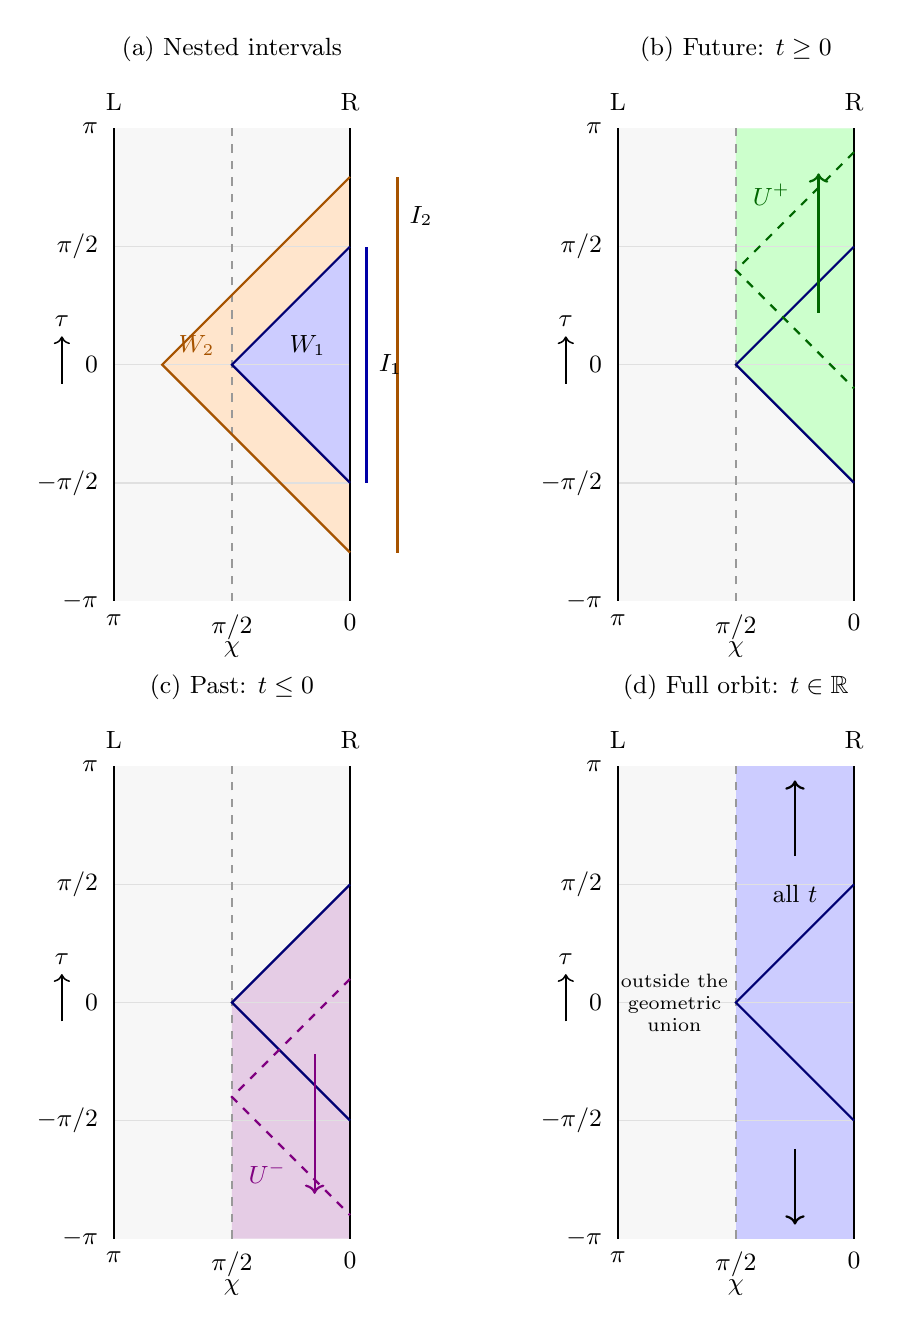
\begin{tikzpicture}[x=3cm,y=3cm,line width=.55pt,font=\small]
 % Common coordinates: x=1-chi/pi, y=tau/pi.
 \foreach \xx/\yy/\mode in {0/8.1/0,6.4/8.1/1,0/0/2,6.4/0/3}{
  \begin{scope}[shift={(\xx cm,\yy cm)}]
   \fill[black!3] (0,-1) rectangle (1,1);
   \ifcase\mode
    \fill[orange!20] (1,.795167) -- (.204833,0) -- (1,-.795167) -- cycle;
    \fill[blue!20] (1,.5) -- (.5,0) -- (1,-.5) -- cycle;
   \or
    \fill[green!20] (1,-.5) -- (1,1) -- (.5,1) -- (.5,0) -- cycle;
   \or
    \fill[violet!20] (1,.5) -- (.5,0) -- (.5,-1) -- (1,-1) -- cycle;
   \or
    \fill[blue!20] (.5,-1) rectangle (1,1);
   \fi
   \foreach \v in {-.5,0,.5}{\draw[black!12] (0,\v)--(1,\v);}
   \draw[dashed,black!40] (.5,-1)--(.5,1);
   \draw[thick] (0,-1)--(0,1) (1,-1)--(1,1);
   \draw[thick,blue!45!black] (1,.5)--(.5,0)--(1,-.5);
   \foreach \v/\lab in {-1/{-\pi},-.5/{-\pi/2},0/0,.5/{\pi/2},1/\pi}{
    \node[anchor=east] at (-.025,\v) {$\lab$};
   }
   \foreach \v/\lab in {0/\pi,.5/{\pi/2},1/0}{
    \node[below] at (\v,-1.015) {$\lab$};
   }
   \node[below] at (.5,-1.13) {$\chi$};
   \node[above] at (0,1.035) {L};
   \node[above] at (1,1.035) {R};
   \draw[->] (-.22,-.08)--(-.22,.12) node[above] {$\tau$};
   \ifcase\mode
    \node[above] at (.5,1.24) {(a) Nested intervals};
    \draw[orange!65!black,thick]
     (1,.795167)--(.204833,0)--(1,-.795167);
    \draw[blue!65!black,very thick] (1.07,-.5)--(1.07,.5);
    \draw[orange!65!black,very thick] (1.2,-.795167)--(1.2,.795167);
    \node[right] at (1.08,0) {$I_1$};
    \node[right] at (1.21,.63) {$I_2$};
    \node at (.82,.08) {$W_1$};
    \node[orange!65!black] at (.35,.08) {$W_2$};
   \or
    \node[above] at (.5,1.24) {(b) Future: $t\ge0$};
    \draw[dashed,green!40!black,thick] (1,.9)--(.5,.4)--(1,-.1);
    \draw[->,green!40!black,thick] (.85,.22)--(.85,.81);
    \node[green!40!black] at (.65,.72) {$U^+$};
   \or
    \node[above] at (.5,1.24) {(c) Past: $t\le0$};
    \draw[dashed,violet,thick] (1,.1)--(.5,-.4)--(1,-.9);
    \draw[->,violet,thick] (.85,-.22)--(.85,-.81);
    \node[violet] at (.65,-.72) {$U^-$};
   \or
    \node[above] at (.5,1.24) {(d) Full orbit: $t\in\mathbb R$};
    \draw[->,thick] (.75,.62)--(.75,.94);
    \draw[->,thick] (.75,-.62)--(.75,-.94);
    \node at (.75,.46) {all $t$};
    \node[align=center,text width=1.4cm,font=\scriptsize] at (.24,0)
     {outside the geometric union};
   \fi
  \end{scope}
 }
 \end{tikzpicture}
 \caption{Inclusion-Hamiltonian histories at $\alpha=1/4$ for the
 Poincar\'e pair $(-1,1)\subset(-3,3)$. The chosen boundary is R,
 at $\chi=0$. In global boundary time the intervals have endpoints
 $\pm\pi/2$ and $\pm2\arctan3$, respectively. The solid inner null
 edges bound the original wedge $W_1$; the dashed colored edges show
 sample translates. Green and violet shading indicate the future and
 past sweeps. Their union is the proper strip $0<\chi<\pi/2$.
 The displayed time range is finite, but global time continues to
 $\pm\infty$. The unshaded half in panel (d) is outside the geometric
 union, not its causal complement.}
 \label{fig:ads2-inclusion-histories}
\end{figure}

The fact that $U_\alpha$ is a proper region does not imply that its
causal completion is proper. If $O^\perp$ denotes the set of bulk
points spacelike to every point of $O$, then
\begin{equation}
 U_\alpha^\perp=\varnothing,
 \qquad
 U_\alpha^{\perp\perp}=\mathrm{AdS}_2.
 \label{eq:ads2-history-causal-completion}
\end{equation}
For any bulk point, a point in $U_\alpha$ sufficiently far in its
future is timelike related to it. In particular, the opposite boundary
is not spacelike separated from the all-time strip.

\paragraph{Generated algebras, standardness, and invariant cores.}
Define the future and past history algebras and the corresponding
intersections by
\begin{equation}
 \mathcal A_\alpha^\pm
 :=\bigvee_{\pm t\ge0}\gamma_t^\alpha(\mathcal A_{I_1}),
 \qquad
 \mathcal C_\alpha^\pm
 :=\bigcap_{\pm t\ge0}\gamma_t^\alpha(\mathcal A_{I_1}).
 \label{eq:ads2-history-algebras}
\end{equation}
Geometric covariance identifies the two-sided history with the algebra
generated by the wedge algebras in $U_\alpha$. Empty causal complement
alone need not make this algebra irreducible for an arbitrary net.
For the free field, irreducibility follows directly from the global
normal modes:
\begin{equation}
 \Phi(\tau,\chi)
 =\sum_{n\ge0}f_n(\chi)
 \left[b_n e^{-i(\Delta+n)\tau}
       +b_n^\dagger e^{i(\Delta+n)\tau}\right].
 \label{eq:ads2-history-modes}
\end{equation}
Each $f_n$ is analytic in the bulk and does not vanish identically on
any open radial interval. Smearing in such an interval and using
arbitrarily long time smearings isolates the two quadratures of each
mode, in the closure of the one-particle real subspace. Their Weyl
operators generate the irreducible Fock representation. Consequently,
\begin{equation}
 \boxed{
 \bigvee_{t\in\mathbb R}\gamma_t^\alpha(\mathcal A_{I_1})
 =\mathcal A(U_\alpha)=B(\mathcal H_{\rm bulk}).
 }
 \label{eq:ads2-history-full-generation}
\end{equation}
This is algebraic generation by observations in a timelike strip;
it does not assert that the geometric union equals all of spacetime.

Standardness is consistent with this conclusion. In the original
Poincar\'e frame, $W_a=\{z>0:|T|+z<a\}$, and the relative commutant
contains the algebra of the nonempty diamond
\begin{equation}
 D_{r,R}=\{(T,z):r+|T|<z<R-|T|\}
 \subset W_R\cap W_r^\perp .
\end{equation}
The vacuum is cyclic for this diamond by Reeh--Schlieder, hence for
$\mathcal A_{I_1}'\cap\mathcal A_{I_2}$. It is separating because this
relative commutant lies in $\mathcal A_{I_2}$. Thus the inclusion is
standard. For these factors, its ambient modular core is
trivial~\cite{companion}:
\begin{equation}
 \bigcap_{s\in\mathbb R}
 \sigma_s^{\mathcal A_{I_2}}(\mathcal A_{I_1})=\mathbb C1.
 \label{eq:ads2-history-modular-core}
\end{equation}
This modular core is distinct from the intersections in
\eqref{eq:ads2-history-algebras}.

\paragraph{Nuclearity and one-sided generation.}
The spectrum also gives a direct check of $L^2$-nuclearity. Since
$L_0^{(a_\alpha)}$ is unitarily equivalent to global energy,
\begin{equation}
 \|X_\alpha\|_1
 =\operatorname{Tr}\rho_\alpha^{1/2}
 =\prod_{n=0}^\infty
   \frac{1}{1-e^{-\lambda_\alpha(\Delta+n)}}<\infty.
 \label{eq:ads2-history-nuclearity}
\end{equation}
The convergence holds for $\Delta>0$, $\ell>0$, and
$0<\alpha<1/2$. At the midpoint it reproduces the nuclearity index
with $\lambda_{1/4}=\ell$, in agreement with the positive-energy
group calculation of Buchholz, D'Antoni and Longo~\cite{BDL2007}.
In particular, $\rho_\alpha$ has full support and $H_\alpha$ has pure
point spectrum. Strong recurrence then approximates every negative
time evolution by positive times, and conversely. Combining this
with \eqref{eq:ads2-history-full-generation} gives
\begin{equation}
 \boxed{
 \mathcal A_\alpha^+
 =\mathcal A_\alpha^-
 =B(\mathcal H_{\rm bulk}).
 }
 \label{eq:ads2-history-one-sided-generation}
\end{equation}

There is no nontrivial invariant core hidden in the strip. To see
this without identifying algebraic intersections with intersections
of regions, let
$\mathcal C_\alpha=\bigcap_{t\in\mathbb R}
\gamma_t^\alpha(\mathcal A_{I_1})$.
This algebra is invariant, and the vacuum is separating for it.
On $\overline{\mathcal C_\alpha\Omega}$ it is also cyclic, and its
modular conjugation sends the restricted $H_\alpha$ to its negative.
Positivity therefore forces that restriction to vanish. Since the
Fock vacuum is the unique zero-energy vector,
$\mathcal C_\alpha=\mathbb C1$. The same recurrence identifies both
one-sided intersections with the two-sided one, so
\begin{equation}
 \mathcal C_\alpha^+
 =\mathcal C_\alpha^-
 =\mathcal C_\alpha=\mathbb C1.
 \label{eq:ads2-history-trivial-cores}
\end{equation}
Thus a proper geometric sweep, standardness, trivial cores, and
one-sided generation of the full bulk operator algebra coexist in
this example. The trace estimate uses a single field with
$\Delta>0$; an infinite collection of species or a zero mode requires
a separate spectral analysis.



\section{Subsystem flows in conformal perturbation theory}\label{section:conformalperturbation}

Wedge modular flow remains geometric in the vacuum of a relativistic QFT with the Bisognano--Wichmann property. For a ball, this geometric action generally fails away from a conformal fixed point. We compute its leading correction by perturbing a CFT with a Hermitian scalar primary $O_0$ of dimension $\Delta$. We work in $1+1$ dimensions and use
\begin{equation}
 \mathcal{L}_\lambda=\mathcal{L}_{\mathrm{CFT}}-\lambda O_0,
 \qquad S_{E,\lambda}=S_{E,0}+\lambda\int d^2x_E\,O_0(x_E).
 \label{eq:cpt-deformation}
\end{equation}
The Euclidean sign fixes the signs of both the modular-Hamiltonian and vacuum corrections below. We use a common regulated description of the theories, with a fixed identification of the external operators. We assume that the regulated density matrices are faithful and their first variations exist. Continuum formulas are conditional on a renormalized distributional extension of the ordered correlators and contact terms; its existence and infrared limit depend on the theory. The expansion is in regulated correlation functions at fixed modular time; it need not be uniform at large time or in the infinite-volume limit. We use $3/2<\Delta<2$ for the pointwise kernel formulas below; the joint geometric integral has the weaker condition $\Delta>1$, as explained after Lemma~\ref{lem:cpt-ball-flow}.

\subsection{Perturbation of ball modular flow}

Let $I=(-1,1)$ at $t=0$ and let $B$ be its causal development. In a regulated description, write $k_{B,\lambda}=-\log\rho_{B,\lambda}$ for the one-sided modular Hamiltonian. Its adjoint action on $\mathcal A(B)$ agrees with that of the full generator $K_{B,\lambda}=-\log\Delta_{B,\lambda}$. We distinguish these generators because only the full modular operator acts on the vacuum Hilbert space with $\Delta_{B,\lambda}|\Omega_\lambda\rangle=|\Omega_\lambda\rangle$.

The first-order logarithmic variation is \cite{BalakrishnanParrikar2020}
\begin{align}
 \delta k_B&=\int_{-\infty+i\theta}^{\infty+i\theta}
 \frac{2\pi\,du}{4\sinh^2(\pi u)}
 e^{iu k_{B,0}}\rho_{B,0}^{-1}\delta\rho_B e^{-iu k_{B,0}},
 \qquad 0<\theta<1,\nonumber\\
 \rho_{B,0}^{-1}\delta\rho_B
 &=-\lambda\int_{-1}^1dX\int_0^1d\tau\,
 J(\tau,X)\Omega^\Delta(-i\tau,X)
 e^{\tau k_{B,0}}O_0(0,X)e^{-\tau k_{B,0}}.
 \label{eq:cpt-density-variation}
\end{align}
Here and below we suppress scalar terms from density-matrix normalization: they drop out of the adjoint flow. The contour and endpoint prescriptions are part of the distributional definition of the kernel.

For real $u$, define $\beta_C^u=\operatorname{Ad}\Delta_{C,0}^{-iu}$, so $\beta_C^u=\sigma_C^{-u}$ with the convention \eqref{eq:modular-flow}. For an insertion at $(0,X)$ in the unit ball,
\begin{gather}
 \beta_B^u(O_0(0,X))=\Omega^{-\Delta}(u,X)O_0(t_u,x_u),\nonumber\\
 t_u=\frac{(1-X^2)\sinh(2\pi u)}{2\Omega(u,X)},
 \qquad x_u=\frac{X}{\Omega(u,X)},\nonumber\\
 \Omega(u,X)=1+(1-X^2)\sinh^2(\pi u).
 \label{eq:cpt-ball-flow}
\end{gather}
The positive Euclidean Jacobian is
\begin{equation}
 J(\tau,X)=\left|\det\frac{\partial(t_E,x_E)}{\partial(\tau,X)}\right|
 =\frac{\pi(1-X^2)}{\Omega^2(-i\tau,X)},
 \qquad \Omega(-i\tau,X)=1-(1-X^2)\sin^2(\pi\tau).
 \label{eq:cpt-euclidean-jacobian}
\end{equation}
Thus $J$ is a Euclidean measure factor, rather than the Lorentzian determinant evaluated at complex time. Choosing $\theta=\tau$ in each insertion removes the Euclidean evolution from the operator and gives
\begin{align}
 \delta k_B&=\pi\lambda\int_{-1}^1dX\int_{\mathbb R}du\,
 h(u,X)\beta_B^u(O_0(0,X)),\label{eq:deltaK}\\
 h(u,X)&=-\frac{\pi(1-X^2)}{2}\int_0^1d\tau\,
 \frac{\Omega^{\Delta-2}(-i\tau,X)}{\sinh^2(\pi(u+i\tau))}.
 \label{eq:cpt-h-kernel}
\end{align}

The kernel contains a local term. With the same endpoint prescription,
\begin{equation}
 -\frac{\pi}{2}\int_0^1\frac{d\tau}{\sinh^2(\pi(u+i\tau))}=\delta(u),
 \label{eq:cpt-delta-kernel}
\end{equation}
as an identity of distributions in $u$, not a pointwise identity. Accordingly,
\begin{align}
 h(u,X)&=(1-X^2)\bigl[\delta(u)+h_{\mathrm{reg}}(u,X)\bigr],\nonumber\\
 h_{\mathrm{reg}}(u,X)&=-\frac{\pi}{2}\int_0^1d\tau\,
 \frac{\Omega^{\Delta-2}(-i\tau,X)-1}{\sinh^2(\pi(u+i\tau))}.
 \label{eq:cpt-regular-kernel}
\end{align}
The local contribution is $\pi\lambda\int_{-1}^1dX(1-X^2)O_0(0,X)$; the remaining term spreads the perturbation along the unperturbed modular orbit. At $\Delta=2$ this nonlocal kernel vanishes formally at first order. A dimension-two operator need not be exactly marginal, so this observation alone does not imply that the deformed theory is another CFT.

Write $k_{B,\lambda}=k_{B,0}+\lambda k_B^{(1)}+O(\lambda^2)$ and introduce the interaction-picture flow
\begin{equation}
 u_{s,\lambda}=e^{-is k_{B,0}}e^{is k_{B,\lambda}}
 =1+\lambda u_s^{(1)}+O(\lambda^2),
 \qquad u_s^{(1)}=i\int_0^s dw\,\beta_B^{-w}(k_B^{(1)}).
 \label{eq:cpt-interaction-flow}
\end{equation}
Duhamel's formula and a shift of the real modular integration variable give the following result.
\begin{lemma}[Perturbed modular flow of the unit ball]
\label{lem:cpt-ball-flow}
For the regulated perturbation \eqref{eq:cpt-deformation}, and real $s$,
\begin{align}
 u_{s,\lambda}&=1+i\pi\lambda\int_{-1}^1dX\int_{\mathbb R}du\,
 (1-X^2)Q(u,X;s)\Omega^{-\Delta}(u,X)O_0(t_u,x_u)
 +O(\lambda^2),\label{eq:cpt-flow-correction}\\
 Q(u,X;s)&=Q_{\mathrm{loc}}(u;s)+Q_{\mathrm{nonloc}}(u,X;s),\nonumber\\
 Q_{\mathrm{loc}}(u;s)&=\int_0^s dw\,\delta(u+w),\nonumber\\
 Q_{\mathrm{nonloc}}(u,X;s)&=-\frac{\pi}{2}\int_0^s dw\int_0^1d\tau\,
 \frac{\Omega^{\Delta-2}(-i\tau,X)-1}{\sinh^2(\pi(u+w+i\tau))}.
 \label{eq:cpt-Q-kernel}
\end{align}
For $s>0$, $Q_{\mathrm{loc}}=\mathbf 1_{(-s,0)}$; for $s<0$, it is $-\mathbf 1_{(0,-s)}$. For $3/2<\Delta<2$, integrating over $w$ yields
\begin{align}
 Q_{\mathrm{nonloc}}(u,X;s)
 &=\frac12\int_0^1d\tau\,[\Omega^{\Delta-2}(-i\tau,X)-1]\nonumber\\
 &\quad\times\bigl[\coth(\pi(u+s+i\tau))-\coth(\pi(u+i\tau))\bigr].
 \label{eq:cpt-Q-coth}
\end{align}
The integrals retain their distributional prescription at the endpoints. The remainder is understood in regulated correlation functions at fixed $s$.
\end{lemma}

The subtraction in \eqref{eq:cpt-regular-kernel} removes the endpoint singularity associated with the local term. A separate issue occurs at $X=0$, $\tau=1/2$, where the Euclidean map reaches infinity and $\Omega$ vanishes. Locally,
\[
 \Omega(-i\tau,X)\simeq X^2+\pi^2(\tau-1/2)^2.
\]
The joint $(X,\tau)$ integral of $\Omega^{\Delta-2}$ is locally integrable for $\Delta>1$, whereas the $\tau$ integral at fixed $X=0$ requires $\Delta>3/2$. We use the latter range for the pointwise kernel formulas. These conditions do not replace the contact-term prescriptions needed when the kernel is inserted in a correlation function. For a ball of radius $r$, the expansion parameter is the dimensionless coupling $\lambda r^{2-\Delta}$.

\paragraph{Almost-marginal relevant operators:}
Let $\epsilon=2-\Delta>0$ be small. The leading nonlocal correction can be evaluated explicitly:
\begin{align}
 \Omega^{-\epsilon}(-i\tau,X)-1
 &=-\epsilon\log\Omega(-i\tau,X)+O(\epsilon^2),\nonumber\\
 -\log\Omega(-i\tau,X)&=\sum_{n\in\mathbb Z}a_n^{(1)}(X)e^{2\pi in\tau},\nonumber\\
 a_0^{(1)}(X)&=-2\log\frac{1+|X|}{2},\nonumber\\
 a_{n\ne0}^{(1)}(X)&=\frac1{|n|}
 \left(-\frac{1-|X|}{1+|X|}\right)^{|n|}.
 \label{eq:cpt-near-marginal-Fourier}
\end{align}
At $X=0$ the Fourier expansion is interpreted in the integrable sense. The expansion in $\epsilon$ is not pointwise uniform near $\Omega=0$, but its logarithmic coefficients are integrable. For $0\leq\epsilon\leq\epsilon_0<1/2$, an integrable bound by $\Omega^{-\epsilon_0}\log^2\Omega$ controls the remainder in the $\tau$ integral, including $X=0$.

For real $v$, set
\begin{equation}
 L(v,X)=\log\left(\frac{1+|X|+(1-|X|)e^{-2\pi|v|}}{2}\right).
\end{equation}
Expanding $\coth$ on either side of $v=0$ and pairing its Fourier modes with \eqref{eq:cpt-near-marginal-Fourier} gives
\begin{align}
 &\int_0^1d\tau\,[\Omega^{-\epsilon}(-i\tau,X)-1]
 \coth(\pi(v+i\tau))\nonumber\\
 &\qquad=-2\epsilon\operatorname{sgn}(v)L(v,X)+O(\epsilon^2),\nonumber\\
 Q_{\mathrm{nonloc}}(u,X;s)
 &=-\epsilon\operatorname{sgn}(u+s)L(u+s,X)\nonumber\\
 &\quad+\epsilon\operatorname{sgn}(u)L(u,X)+O(\epsilon^2).
 \label{eq:cpt-near-marginal-Q}
\end{align}
This single expression covers all three real-time intervals and vanishes at $s=0$. In particular, the middle interval contains the product of the two logarithm arguments, each with its factor of $1/2$. The local term is unchanged. These real-time expressions, which contain absolute values and sign functions, are not formulas for direct substitution of complex $s$.

\subsection{First-order correction to the characteristic matrix element}

Let $B$ be the unit double cone and let $A$ be the right wedge with endpoint $(0,-x_w)$, with $x_w>1$. This guarantees $B\subset A$. Take fixed Hermitian scalar insertions $O_1(x)$ and $O_2(y)$ with $x\in A$, $y\in B$, understood as regulated or smeared fields. In the common perturbative description, write
\begin{align}
 F_\lambda(z)&=\langle O_1|\Delta_{A,\lambda}^{1/2}
 D_{B\subset A,\lambda}(-z)|O_2\rangle_\lambda\nonumber\\
 &=\langle O_1|\Delta_{A,\lambda}^{1/2+iz}
 \Delta_{B,\lambda}^{-iz}|O_2\rangle_\lambda
 =F_0(z)+\lambda F^{(1)}(z)+O(\lambda^2).
 \label{eq:cpt-characteristic-expansion}
\end{align}
Here $D_{B\subset A,\lambda}(z)=\Delta_{A,\lambda}^{-iz}\Delta_{B,\lambda}^{iz}$, and $F_\lambda$ is the unnormalized matrix element. Even when both regions are wedges, only the spacetime action remains the same as in the CFT: the vacuum correlation function generally changes with $\lambda$.

For real $t$, wedge modular conjugation sends $O_1(x)$ to its reflected operator $O_1(x_J)$, with any internal conjugation included. Since the wedge flow is geometric, Tomita's relation gives
\begin{equation}
 F_\lambda(t)=\langle\Omega_\lambda|
 \beta_A^t(O_1(x_J))\,
 \beta_B^t\bigl(u_{t,\lambda}O_2(y)u_{t,\lambda}^\dagger\bigr)
 |\Omega_\lambda\rangle.
 \label{eq:cpt-real-characteristic}
\end{equation}
We fix the perturbative identification so that the displayed wedge action and reflected external operator have no explicit coupling variation. Any additional external-operator counterterms must be included if a different identification is used.

Choose normalized vacua with $\langle\Omega_0|\Omega^{(1)}\rangle=0$. The Euclidean preparation in \eqref{eq:cpt-deformation} gives
\begin{align}
 |\Omega_\lambda\rangle&=|\Omega_0\rangle+\lambda|\Omega^{(1)}\rangle+O(\lambda^2),\nonumber\\
 |\Omega^{(1)}\rangle&=-\int_{\mathbb R}dX\int_{-\infty}^0d\tau\,
 O_{0,c}(-i\tau,X)|\Omega_0\rangle,
 \qquad O_{0,c}=O_0-\langle O_0\rangle_0.
 \label{eq:cpt-vacuum-variation}
\end{align}
This is a regulated preparation formula; an infinite-volume derivative need not exist as a Hilbert-space vector. The vacuum subtraction accounts for normalization.

Set $G_{12}(t)=\beta_A^t(O_1(x_J))\beta_B^t(O_2(y))$. There are three first-order contributions:
\begin{align}
 F^{(1)}(t)&=F^{(1)}_{\mathrm{flow}}(t)
 +F^{(1)}_{\mathrm{bra}}(t)+F^{(1)}_{\mathrm{ket}}(t),\nonumber\\
 F^{(1)}_{\mathrm{flow}}(t)
 &=\langle\Omega_0|\beta_A^t(O_1(x_J))
 \beta_B^t([u_t^{(1)},O_2(y)])|\Omega_0\rangle,\nonumber\\
 F^{(1)}_{\mathrm{bra}}(t)&=\langle\Omega^{(1)}|G_{12}(t)|\Omega_0\rangle,\nonumber\\
 F^{(1)}_{\mathrm{ket}}(t)&=\langle\Omega_0|G_{12}(t)|\Omega^{(1)}\rangle.
 \label{eq:cpt-three-corrections}
\end{align}
Using invariance of the CFT vacuum under the full unperturbed modular flow, the flow term becomes
\begin{align}
 F^{(1)}_{\mathrm{flow}}(t)
 &=i\pi\int_{-1}^1dX\int_{\mathbb R}du\,
 (1-X^2)Q(u,X;t)\Omega^{-\Delta}(u,X)\nonumber\\
 &\quad\times\langle\Omega_0|
 (\beta_B^{-t}\circ\beta_A^t)(O_1(x_J))
 [O_0(t_u,x_u),O_2(y)]|\Omega_0\rangle.
 \label{eq:cpt-flow-three-point}
\end{align}
All three terms reduce to ordered CFT three-point functions, together with the required subtractions and contact terms. For scalar primaries their separated-point form is fixed up to CFT data:
\begin{equation}
 \langle O_1(x_1)O_2(x_2)O_3(x_3)\rangle_0
 =\frac{C_{123}}
 {(x_{12}^2)^{(\Delta_1+\Delta_2-\Delta_3)/2}
  (x_{23}^2)^{(\Delta_2+\Delta_3-\Delta_1)/2}
  (x_{31}^2)^{(\Delta_3+\Delta_1-\Delta_2)/2}}.
 \label{eq:cpt-scalar-three-point}
\end{equation}
For the displayed Lorentzian ordering,
\begin{equation}
 x_{ij}^2=-(t_i-t_j-i(\epsilon_i-\epsilon_j))^2+(x_i-x_j)^2,
 \qquad \epsilon_1>\epsilon_2>\epsilon_3\to0^+.
\end{equation}
The two terms in the commutator have their respective ordering prescriptions. Conformal Jacobians follow from the modular transformations in \eqref{eq:cpt-three-corrections} and \eqref{eq:cpt-flow-three-point}. The dimensions and $C_{123}$, as well as possible contact terms, depend on the CFT; the integrated correction is therefore not theory-independent.

Microcausality restricts \eqref{eq:cpt-flow-three-point} to insertions $O_0$ that are causally related to $O_2$. Moving $O_2$ toward the entangling surface can reduce this region, suggesting a local boost approximation. Its volume alone does not bound the correction, since the kernel and correlator can become singular in the same limit. Section~\ref{section:approx} gives a separate nonperturbative estimate with specified localization and topology.

\paragraph{Two checks. \KL{(?)}}
Two features of \eqref{eq:cpt-three-corrections} are worth isolating. First, if both regions are wedges, the Bisognano--Wichmann property holds at every $\lambda$, so the modular flows are geometric for all couplings, $u^{(1)}_t=0$, and $F^{(1)}_{\mathrm{flow}}\equiv0$. \KL{(Is it true that $u^{(1)}_t=0$? I thought the first order term will be the difference of the action, which make the original boost generator to be the new boost generator.)} The entire first-order correction is then $F^{(1)}_{\mathrm{bra}}+F^{(1)}_{\mathrm{ket}}$, the conformal perturbation of the two-point function at the geometrically fixed points of \eqref{eq:F-reflected}: the operator \eqref{eq:wedge-characteristic} is unchanged and only the correlator moves. For the double cone, by contrast, the flow term is the genuinely new contribution and encodes the departure of the inner modular flow from geometry. Second, the pointwise kernel formulas require $3/2<\Delta<2$, which excludes the free mass deformations ($\Delta=0$ for $\phi^2$ of a free boson in two dimensions and $\Delta=1$ for $\bar\psi\psi$ of a free fermion). The exact massive result of Lemma~\ref{lem:massive-free-boson} therefore cannot be used as a check of the perturbative formulas in their present range; extending the kernel analysis to $1<\Delta\le3/2$ through the joint $(X,\tau)$ integral is the step that would make such a comparison possible.

Finally, normalize as in the preceding section:
\begin{equation}
 f_\lambda=\frac{F_\lambda}{N_\lambda},
 \qquad f^{(1)}=\frac{F^{(1)}}{N_0}-\frac{F_0N^{(1)}}{N_0^2},
 \qquad N^{(1)}=\left.\partial_\lambda N_\lambda\right|_{\lambda=0}.
 \label{eq:cpt-normalized-correction}
\end{equation}
For each coupling, finite quarter-modular norms ensure that the exact $f_\lambda$ is analytic and bounded by one on the centered strip. Analyticity of its perturbative coefficient additionally requires differentiation locally uniformly in that strip. Null singularities of individual three-point integrands do not by themselves establish singularities of the integrated answer: contour pinches, ordering prescriptions, and renormalization must be analyzed. Smearing controls the external fields, but does not automatically remove every contact divergence. We therefore obtain the real-time first-order formula above without claiming an additional complex singularity classification.

% =====================================================================
\section{Nonperturbative bounds on subsystem flows of double cones}\label{section:approx}

We now compare subregion flows of large double cones with those of wedges. The physical idea is that a fixed local observable remains inside the large double cone for an increasingly long interval of wedge modular time. Fredenhagen's estimate \cite{fredenhagen} turns this geometric fact into a bound on time-averaged modular evolution. We first state a uniform estimate on localized vectors, then distinguish it from strong convergence on each fixed vector for an increasing exhaustion of a wedge.

Work in a vacuum representation of a Poincar\'e-covariant local net, and assume the Bisognano--Wichmann property in addition to isotony and locality. The vacuum is cyclic and separating for the double-cone and wedge algebras used below. Wedge algebras are generated by their bounded subregions. These assumptions make both geometric wedge flow and modular convergence available; geometric modular action does not follow from the Haag--Kastler axioms alone.

Let
\begin{equation}
 W_0=\{x:|x_0|<x_1\},\qquad
 W_r=\{x:|x_0|<x_1-r\},\qquad r>0.
\end{equation}
If $T_r$ implements translation by $r$ along $x_1$, covariance and vacuum invariance give
\begin{equation}
 \mathcal A(W_r)=\operatorname{Ad}_{T_r}\mathcal A(W_0),
 \qquad \Delta_{W_r}^{it}=T_r\Delta_{W_0}^{it}T_r^*.
\end{equation}
Write $B_{c,R}$ for the double cone whose $x_0=0$ section is the ball of radius $R$ centered at $(c,0,\ldots,0)$, with $c\geq R>0$. We use
\begin{equation}
 B_R:=B_{R,R},\qquad B_R^r:=T_r(B_R),\qquad
 B_{e^{\pm2\pi s}R}:=B_{e^{\pm2\pi s}R,e^{\pm2\pi s}R}.
 \label{eq:approx-ball-notation}
\end{equation}
Thus a dilation changes both the center and radius. The shrinking cones approach the wedge vertex, while the increasing family $B_{e^{2\pi s}R}$ exhausts $W_0$. A shrinking ball with its center fixed at $R$ would describe a different geometry.

\subsection{Fredenhagen's estimate and an increasing-ball version}

For a local operator $A$, abbreviate
\begin{equation}
 q(A)=\bigl(\|A\Omega\|^2+\|A^*\Omega\|^2\bigr)^{1/2}.
\end{equation}
Fredenhagen's approximation takes the following form \cite{fredenhagen}.
\begin{theorem}[Fredenhagen]\label{thm:fredenhagen}
For $f\in L^1(\mathbb R)$ and $s>0$, there is $c_f(s)\geq0$, with $c_f(s)\to0$ as $s\to\infty$, such that
\begin{equation}
 \left\|\int_{\mathbb R}dt\,f(t)
 (\Delta_{B_R}^{-it}-\Delta_{W_0}^{-it})A\Omega\right\|^2
 \leq c_f(s)q(A)^2,
 \qquad A\in\mathcal A(B_{e^{-2\pi s}R}).
\end{equation}
\end{theorem}
This is a Hilbert-space norm estimate for a modular-time average, not an operator-norm estimate or a pointwise-in-time bound. Shrinking the support toward the wedge vertex lengthens the interval during which its boosted images remain in $B_R$.

The input to this estimate is the following resolvent bound.
\begin{proposition}\label{prop:resolvent}
Let $\mathcal B\subset\mathcal A$ have a common cyclic and separating vector $\Omega$. If $O\in\mathcal B$ and
\[
 \Delta_\mathcal A^{it}O\Delta_\mathcal A^{-it}\in\mathcal B
 \quad\text{for all }|t|<t_0,
\]
then
\begin{equation}
 \left\|\bigl[(1+\Delta_\mathcal A)^{-1}
 -(1+\Delta_\mathcal B)^{-1}\bigr]O\Omega\right\|
 \leq\eta(t_0)q(O),
 \qquad \eta(t_0)=\frac2\pi\operatorname{arctanh}(e^{-\pi t_0}).
 \label{eq:approx-resolvent}
\end{equation}
\end{proposition}
\begin{proof}
Equip $\operatorname{Dom}S_\mathcal A$ with the Tomita graph norm and let $I$ be its inclusion into $\mathcal H$. The subspace $\operatorname{Dom}S_\mathcal B$ is closed in this graph norm; denote its orthogonal projection by $P_\mathcal B$. The graph-projection identity is
\[
 (1+\Delta_\mathcal A)^{-1}-(1+\Delta_\mathcal B)^{-1}
 =I(1-P_\mathcal B)I^*.
\]
In the Mellin representation of the resolvent, the orbit assumption removes the part with $|t|<t_0$. The remaining modular orbit has graph norm $q(O)$, and $\|I\|\leq1$, giving
\[
 \left\|I(1-P_\mathcal B)I^*O\Omega\right\|
 \leq\frac12\int_{|t|\geq t_0}\frac{dt}{|\sinh(\pi t)|}\,q(O)
 =\eta(t_0)q(O).
\]
This is the resolvent argument of Fredenhagen; the graph identity and Mellin representation are also given in \cite[Section~3]{Hollands2019Edge}.
\end{proof}

For the remainder of the section the support stays fixed, while the containing ball grows.
\begin{corollary}\label{cor:growing-resolvent}
For $O\in\mathcal A(B_R)$,
\begin{equation}
 \left\|\bigl[(1+\Delta_{B_{e^{2\pi s}R}})^{-1}
 -(1+\Delta_{W_0})^{-1}\bigr]O\Omega\right\|
 \leq\eta(s)q(O).
 \label{eq:approx-growing-resolvent}
\end{equation}
\end{corollary}
\begin{proof}
The wedge boost sends $B_R$ into $B_{e^{2\pi s}R}$ for $|t|<s$; the geometric inclusion is verified in Appendix~\ref{app:orbit}. Isotony gives the orbit condition in \eqref{eq:approx-resolvent}, with $\mathcal A=\mathcal A(W_0)$ and $\mathcal B=\mathcal A(B_{e^{2\pi s}R})$.
\end{proof}

The resolvent estimate is quantitative. Since $\operatorname{arctanh}y=\tfrac12\log\frac{1+y}{1-y}\le\frac{y}{1-y}$ for $0\le y<1$,
\begin{equation}
 \eta(s)\le\frac2\pi\,\frac{e^{-\pi s}}{1-e^{-\pi s}},\qquad e^{-\pi s}=\Bigl(\frac{R}{e^{2\pi s}R}\Bigr)^{1/2}:
 \label{eq:eta-rate}
\end{equation}
the resolvent difference on a localized vector decays like the inverse square root of the ratio of the radii. The time-averaged constants $c_f(s)$ below are obtained from \eqref{eq:approx-resolvent} by an approximation argument and are not explicit; in Section~\ref{subsec:cutoff} we compare \eqref{eq:eta-rate} with the explicit rate available when the inner flow is geometric.

Applying the same time-averaging argument to this orbit condition gives the required version of Fredenhagen's theorem.
\begin{theorem}\label{theorem:modifiedfredenhagen}
For $f\in L^1(\mathbb R)$ and $A\in\mathcal A(B_R)$, there is $c_f(s)\geq0$, tending to zero as $s\to\infty$, such that
\begin{equation}
 \left\|\int_{\mathbb R}dt\,f(t)
 (\Delta_{B_{e^{2\pi s}R}}^{-it}-\Delta_{W_0}^{-it})A\Omega\right\|^2
 \leq c_f(s)q(A)^2.
 \label{eq:approx-growing-flow}
\end{equation}
\end{theorem}
\begin{proof}
The proof of the time-averaged estimate uses the modular orbit condition and its resolvent bound. These hold here by the preceding corollary, and $\eta(s)\to0$. Approximation of $f$ in $L^1$ extends the estimate from smooth test functions to all $L^1$ smearings \cite{fredenhagen}.
\end{proof}
Increasing the ambient region suppresses the error for fixed localized vectors and fixed time smearing. This expresses a local boost approximation without assuming a conformal symmetry of the QFT.

\subsection{A double cone inside a wedge}\label{subsection:coneinsidewedge}

Set $B_s^r=B_{e^{2\pi s}R}^r$ and compare
\begin{equation}
 D_{B_s^r\subset W_0}(t)=\Delta_{W_0}^{-it}\Delta_{B_s^r}^{it},
 \qquad D_{W_r\subset W_0}(t)=\Delta_{W_0}^{-it}\Delta_{W_r}^{it}.
\end{equation}
The characteristic operator is a contraction analytic on $0<\operatorname{Im}z<1/2$, with strongly continuous unitary boundary values. Its wedge limit is explicitly geometric, as in Section~\ref{sec:geometric-subregion-flows}.

To obtain a uniform localized bound after multiplication by the outer wedge flow, introduce the spectral family of $L=\log\Delta_{W_0}=-K_{W_0}$:
\begin{equation}
 \Delta_{W_0}^{it}=\int_{\mathbb R}e^{i\mu t}\,dE(\mu),
 \qquad E(\mu)=\mathbf1_{(-\infty,\mu]}(L),
 \qquad F(\mu_0)=E(\mu_0)-E(-\mu_0).
 \label{eq:approx-spectral-cutoff}
\end{equation}
Thus $F(\mu_0)$ projects onto the vectors whose \emph{boost energy}, the generator of the outer wedge flow, lies in $(-\mu_0,\mu_0]$. The spectrum of $L$ is not restricted to nonnegative values. The role of this cutoff is explained in Section~\ref{subsec:cutoff}.

\begin{theorem}\label{theorem:mainresult}
Let $f,tf\in L^1(\mathbb R)$, $\mu_0>0$, and $A\in\mathcal A(B_R^r)$. Then
\begin{equation}
 \left\|F(\mu_0)\int_{\mathbb R}dt\,f(t)
 [D_{B_s^r\subset W_0}(t)-D_{W_r\subset W_0}(t)]A\Omega\right\|^2
 \leq b_f(\mu_0,s)q(A)^2,
 \label{eq:approx-characteristic-bound}
\end{equation}
where $b_f(\mu_0,s)\to0$ for each fixed $f$ and $\mu_0$ as $s\to\infty$. The assumptions include Schwartz functions and compactly supported bounded functions.
\end{theorem}

\begin{lemma}\label{lemma:extensionfredenhagen}
For $g\in L^1(\mathbb R)$ and $A\in\mathcal A(B_R^r)$,
\begin{equation}
 \left\|\int_{\mathbb R}dt\,g(t)
 (\Delta_{B_s^r}^{it}-\Delta_{W_r}^{it})A\Omega\right\|^2
 \leq\widetilde c_g(s)q(A)^2,
 \qquad \widetilde c_g(s)\longrightarrow0.
 \label{eq:approx-translated-flow}
\end{equation}
The constants can be chosen so that $\widetilde c_g(s)^{1/2}\leq2\|g\|_1$ and their convergence is uniform on compact subsets of $L^1(\mathbb R)$.
\end{lemma}
\begin{proof}
Translate $A$ back to $\mathcal A(B_R)$ and use
\[
 \Delta_{B_s^r}^{it}=T_r\Delta_{B_{e^{2\pi s}R}}^{it}T_r^*,
 \qquad T_r\Omega=\Omega.
\]
Translation preserves both terms in $q(A)$. Replacing $t$ by $-t$ in \eqref{eq:approx-growing-flow} supplies the positive-exponent estimate, with the reflected smearing $g(-t)$.

Choose $\widetilde c_g(s)^{1/2}$ to be the optimal bound on the ratio of the norm in \eqref{eq:approx-translated-flow} to $q(A)$. Unitarity gives, for these bounds $a_s(g)$,
\[
 a_s(g)\leq2\|g\|_1,
 \qquad |a_s(g)-a_s(h)|\leq2\|g-h\|_1.
\]
Pointwise convergence and a finite $L^1$ cover of a compact family then give uniform convergence on that family.
\end{proof}

\begin{proof}[Proof of Theorem~\ref{theorem:mainresult}]
Write $V_s(t)=\Delta_{B_s^r}^{it}-\Delta_{W_r}^{it}$ and $f_\mu(t)=e^{-i\mu t}f(t)$. Spectral integration by parts, including both endpoint terms, gives
\begin{equation}
 F(\mu_0)e^{-itL}
 =e^{-i\mu_0t}E(\mu_0)-e^{i\mu_0t}E(-\mu_0)
 +it\int_{-\mu_0}^{\mu_0}d\mu\,e^{-i\mu t}E(\mu).
 \label{eq:approx-spectral-parts}
\end{equation}
Since $\|V_s(t)\|\leq2$ and $f,tf\in L^1$, the resulting ordinary $t$ and $\mu$ integrals are absolutely bounded in norm. Fubini's theorem therefore applies without a formal interchange of two noncommuting spectral measures. Using \eqref{eq:approx-translated-flow},
\begin{align}
 &\left\|F(\mu_0)\int_{\mathbb R}dt\,f(t)e^{-itL}V_s(t)A\Omega\right\|
 \leq B_f(\mu_0,s)q(A),\nonumber\\
 B_f(\mu_0,s)
 &=\widetilde c_{f_{\mu_0}}(s)^{1/2}
 +\widetilde c_{f_{-\mu_0}}(s)^{1/2}
 +\int_{-\mu_0}^{\mu_0}d\mu\,\widetilde c_{tf_\mu}(s)^{1/2}.
 \label{eq:approx-bound-amplitude}
\end{align}
The families $\{f_\mu\}$ and $\{tf_\mu\}$ with $|\mu|\leq\mu_0$ are compact in $L^1$, by continuity in $\mu$. The lemma implies $B_f\to0$, and the squared-norm constant in \eqref{eq:approx-characteristic-bound} is $b_f=B_f^2$.
\end{proof}

For the qualitative limit on a fixed vector, a spectral cutoff is unnecessary. Indeed, the increasing algebras satisfy
\begin{equation}
 \bigvee_{s>0}\mathcal A(B_s^r)=\mathcal A(W_r).
\end{equation}
The modular convergence theorem for increasing algebras with a common cyclic and separating vector gives $\Delta_{B_s^r}^{it}\to\Delta_{W_r}^{it}$ strongly \cite{revolutionizing,takesaki2}; we recall the fixed-vacuum argument in Appendix~\ref{app:convergence}. Consequently, for every $\psi\in\mathcal H$ and $f\in L^1(\mathbb R)$,
\begin{equation}
 \lim_{s\to\infty}\left\|\int_{\mathbb R}dt\,f(t)
 [D_{B_s^r\subset W_0}(t)-D_{W_r\subset W_0}(t)]\psi\right\|=0.
 \label{eq:approx-uncut-wedge-limit}
\end{equation}
Unitarity supplies the dominating bound $2|f(t)|\|\psi\|$. This strong limit gives no rate uniform over all vectors; the preceding theorem supplies uniform control on the specified localized vectors after the spectral cutoff. Its constants need not give an explicit decay rate; the two statements differ in their uniformity and allowed vectors.

\subsection{A double cone inside a double cone}\label{subsection:coneinsidecone}

Let $B_{s,u}=B_{e^{2\pi(s+u)}R}$ and retain $B_s^r=B_{e^{2\pi s}R}^r$. The inclusion diagram is
\begin{equation}
 \begin{tikzcd}
 B_s^r\arrow[r,"\subset"]\arrow[d,"\subset"]
 &B_{s,u}\arrow[d,"\subset"]\\
 W_r\arrow[r,"\subset"]&W_0.
 \end{tikzcd}
\end{equation}
For these balls, strict containment is ensured by
\begin{equation}
 e^{2\pi(s+u)}R>e^{2\pi s}R+\frac r2.
 \label{eq:approx-ball-containment}
\end{equation}
This follows by comparing the center separation with the difference of radii. The stronger condition with $r$ in place of $r/2$ also suffices.

We compare
\begin{equation}
 D_{B_s^r\subset B_{s,u}}(t)=\Delta_{B_{s,u}}^{-it}\Delta_{B_s^r}^{it}
 \quad\text{with}\quad D_{W_r\subset W_0}(t).
\end{equation}

\begin{theorem}\label{theorem:ballinsideball}
Under the assumptions of this section, for every $\psi\in\mathcal H$ and
$f\in L^1(\mathbb R)$,
\begin{equation}
 \lim_{\substack{s\to\infty,\ s+u\to\infty\\ B_s^r\subset B_{s,u}}}
 \left\|\int_{\mathbb R}dt\,f(t)
 [D_{B_s^r\subset B_{s,u}}(t)-D_{W_r\subset W_0}(t)]\psi\right\|=0.
 \label{eq:approx-ball-ball-limit}
\end{equation}
Thus both radii tend to infinity while the inclusion is maintained. In particular,
the iterated limit $u\to\infty$ followed by $s\to\infty$ holds.
\end{theorem}
\begin{proof}
Split the difference as
\begin{align}
 D_{B_s^r\subset B_{s,u}}(t)-D_{W_r\subset W_0}(t)
 &=(\Delta_{B_{s,u}}^{-it}-\Delta_{W_0}^{-it})\Delta_{W_r}^{it}\nonumber\\
 &\quad+\Delta_{B_{s,u}}^{-it}
 (\Delta_{B_s^r}^{it}-\Delta_{W_r}^{it}).
\end{align}
As their radii increase, the two families exhaust $W_0$ and $W_r$, respectively.
Modular strong convergence applies to the fixed vector $\Delta_{W_r}^{it}\psi$
in the first term and to $\psi$ in the second. The prefactor in the second term
is unitary. The norm of the total difference is bounded by $2\|\psi\|$,
so $2|f(t)|\|\psi\|$ gives an integrable bound for dominated convergence.
\end{proof}
This states the large-ball approximation on each fixed vector, without an
operator-norm limit or a rate uniform over the Hilbert-space unit ball.


%\subsection{Why the boost-energy cutoff, and when it can be removed}\label{subsec:cutoff}
\subsection{Role of the boost-energy cutoff}\label{subsec:cutoff}

Theorem~\ref{theorem:mainresult} is uniform over the whole local algebra $\mathcal A(B^r_R)$ but carries the projection $F(\mu_0)$; the strong limit \eqref{eq:approx-uncut-wedge-limit} carries no projection but gives no uniformity. This subsection explains the mechanism, restates the theorem in a form in which the projection is a property of the observer rather than of the state, and shows that the projection can be replaced by a physical assumption on the vectors when the inner modular flow is geometric.

\paragraph{Where the cutoff comes from:}
The quantity to be estimated is
\begin{equation}
 \int_{\mathbb R}dt\,f(t)\bigl[D_{B_s^r\subset W_0}(t)-D_{W_r\subset W_0}(t)\bigr]A\Omega
 =\int_{\mathbb R}dt\,f(t)\,e^{-itL}\,V_s(t)A\Omega,\qquad V_s(t)=\Delta_{B_s^r}^{it}-\Delta_{W_r}^{it}.
 \label{eq:cutoff-quantity}
\end{equation}
Fredenhagen's estimate controls the inner difference $V_s(t)A\Omega$ uniformly over $A$, but only \emph{after} a time average: it is derived from the resolvent bound \eqref{eq:approx-resolvent}, which is a statement about functions of the modular operators, not about the unitaries at a fixed time. In \eqref{eq:cutoff-quantity} the inner difference is multiplied, before the average, by the outer boost $e^{-itL}$. On the spectral component of boost energy $\mu$ this is a phase $e^{-i\mu t}$, so the time average is taken with the smearing function $e^{-i\mu t}f(t)$ instead of $f(t)$, one for each $\mu$. Fredenhagen's constant depends on the smearing function, and the family $\{e^{-i\mu t}f(t)\}_{\mu\in\mathbb R}$ is not compact in $L^1$: a component of large boost energy rotates faster than any fixed time average can resolve, and the spectral integration by parts \eqref{eq:approx-spectral-parts} that organizes the estimate produces an integral $\int d\mu$ over the retained energies. The projection $F(\mu_0)$ restricts to $|\mu|\le\mu_0$, where the family is compact and the constants converge uniformly. Physically, $\mu_0$ is a resolution in boost energy: the comparison of the two subsystem flows is made with the resolution of an observer whose Rindler-energy measurements are bounded by $\mu_0$. Since the boost generator is an energy weighted by the distance from the edge of the wedge, bounded boost energy on vectors localized at bounded distance from the edge is, in effect, an energy bound. \KL{(The last sentence need more justification)}

That the cutoff is a property of the observer and not of the vector $A\Omega$ is made explicit by restating the theorem in weak form.

\begin{corollary}[Probes of bounded boost energy]\label{cor:probes}
Under the hypotheses of Theorem~\ref{theorem:mainresult}, for every $\chi\in F(\mu_0)\mathcal H$ and $A\in\mathcal A(B_R^r)$,
\begin{equation}
 \Bigl|\Bigl\langle\chi\Bigm|\int_{\mathbb R}dt\,f(t)\bigl[D_{B_s^r\subset W_0}(t)-D_{W_r\subset W_0}(t)\bigr]A\Omega\Bigr\rangle\Bigr|
 \le b_f(\mu_0,s)^{1/2}\,\|\chi\|\,q(A).
\end{equation}
\end{corollary}
\begin{proof}
$\chi=F(\mu_0)\chi$ and $F(\mu_0)$ is self-adjoint; apply Cauchy--Schwarz and \eqref{eq:approx-characteristic-bound}.
\end{proof}
The subspace $\bigcup_{\mu_0}F(\mu_0)\mathcal H$ is dense, so the corollary asserts weak convergence of the time-averaged difference, uniformly over localized operators, tested against any probe of bounded boost energy. No probe with finite boost-energy resolution can distinguish the subsystem flow of the large double cone from that of the wedge, up to an error that vanishes as the cone grows.

\paragraph{Trading the cutoff for a pointwise estimate:}
The outer boost is harmless if we have control over the inner difference at each fixed modular time rather than only on average. Unitarity allows us to remove it from the norm.

\begin{proposition}[Pointwise control removes the cutoff]\label{prop:pointwise}
Let $\mathcal V\subset\mathcal H$ be a set of vectors with a seminorm $\mathcal E$, and suppose that for every $T>0$ there is $\epsilon_T(s)\to0$ as $s\to\infty$ with
\begin{equation}
 \sup_{|t|\le T}\bigl\|(\Delta_{B_s^r}^{it}-\Delta_{W_r}^{it})\psi\bigr\|\le\epsilon_T(s)\,\mathcal E(\psi),\qquad\psi\in\mathcal V .
 \label{eq:pointwise-hypothesis}
\end{equation}
Then for $f\in L^1(\mathbb R)$ and $\psi\in\mathcal V$,
\begin{equation}
 \Bigl\|\int_{\mathbb R}dt\,f(t)\bigl[D_{B_s^r\subset W_0}(t)-D_{W_r\subset W_0}(t)\bigr]\psi\Bigr\|
 \le\epsilon_T(s)\,\|f\|_1\,\mathcal E(\psi)+2\|\psi\|\int_{|t|>T}|f(t)|\,dt ,
 \label{eq:pointwise-conclusion}
\end{equation}
with no spectral cutoff and no restriction on the probe.
\end{proposition}
\begin{proof}
$\|e^{-itL}V_s(t)\psi\|=\|V_s(t)\psi\|$ by unitarity of the outer flow; use \eqref{eq:pointwise-hypothesis} for $|t|\le T$ and $\|V_s(t)\|\le2$ otherwise.
\end{proof}
\KL{Maybe bring back the 1+1d CFT calculation where we kind of have a pointwise control}

The content of the proposition is that the boost-energy cutoff is the price of knowing the inner approximation only on average in modular time. Fredenhagen's resolvent method does not supply \eqref{eq:pointwise-hypothesis}, and a pointwise estimate uniform over all of $\mathcal A(B_R^r)$ with $\mathcal E=q$ is not to be expected, since bounded operators can create arbitrarily high energy. The hypothesis is instead a statement about a class of vectors singled out by an energy-type seminorm. When the inner flow is geometric, it holds with an explicit rate.

\begin{theorem}[Pointwise bound in two-dimensional CFT]\label{thm:CFT-pointwise}
Let the net be a $1+1$ dimensional conformal net in its vacuum representation. Let $\hat K_\pm^{(r)}\ge0$ be the self-adjoint generators of the special conformal transformations $u\mapsto u/(1+\lambda u)$ of the two null coordinates measured from the vertex of $W_r$. Then for every $\psi\in\operatorname{Dom}\hat K_+^{(r)}\cap\operatorname{Dom}\hat K_-^{(r)}$ and every $t\in\mathbb R$,
\begin{equation}
 \bigl\|\bigl[D_{B_s^r\subset W_0}(t)-D_{W_r\subset W_0}(t)\bigr]\psi\bigr\|
 \le\frac{e^{2\pi|t|}-1}{2\,e^{2\pi s}R}\Bigl(\|\hat K_+^{(r)}\psi\|+\|\hat K_-^{(r)}\psi\|\Bigr).
 \label{eq:CFT-pointwise}
\end{equation}
In particular \eqref{eq:pointwise-hypothesis} holds with $\mathcal E(\psi)=\|\hat K_+^{(r)}\psi\|+\|\hat K_-^{(r)}\psi\|$ and $\epsilon_T(s)=(e^{2\pi T}-1)/(2e^{2\pi s}R)$, and for $e^{2\pi|t|}f\in L^1$ the time-averaged difference decays as $e^{-2\pi s}$ without any cutoff.
\end{theorem}
\begin{proof}
By translation covariance take $r=0$. In null coordinates $u,v$ measured from the vertex, $B_{e^{2\pi s}R}$ is the product of the intervals $(0,2R_s)$, $R_s=e^{2\pi s}R$, and $W_0$ of the half-lines $(0,\infty)$. The physical modular flow of $W_0$ is the dilation $u\mapsto e^{2\pi t}u$, $v\mapsto e^{-2\pi t}v$. The physical modular flow of the double cone is the M\"obius flow fixing $0$ and $2R_s$ with the same multiplier at $0$~\cite{HislopLongo1982}:
\[
 u\mapsto\frac{2R_s\,u\,e^{2\pi t}}{2R_s+u(e^{2\pi t}-1)},\qquad
 v\mapsto\frac{2R_s\,v\,e^{-2\pi t}}{2R_s+v(e^{-2\pi t}-1)} .
\]
Composing with the inverse dilation gives
\[
 (\phi^{W}_t)^{-1}\circ\phi^{B}_t:\quad u\mapsto\frac{u}{1+\lambda_tu},\quad v\mapsto\frac{v}{1+\lambda'_tv},\qquad
 \lambda_t=\frac{e^{2\pi t}-1}{2R_s},\quad\lambda'_t=\frac{e^{-2\pi t}-1}{2R_s},
\]
a pure special conformal transformation in each chirality. Both modular groups are implemented by the vacuum representation $U$ of the conformal group, with the lift fixed by continuity from $t=0$, so
\[
 \Delta_{B_s}^{-it}=\Delta_{W_0}^{-it}\,e^{-i\lambda_t\hat K_+}e^{-i\lambda'_t\hat K_-},
\]
and $\Delta_{B_s}^{-it}-\Delta_{W_0}^{-it}=\Delta_{W_0}^{-it}\bigl(e^{-i\lambda_t\hat K_+}e^{-i\lambda'_t\hat K_-}-1\bigr)$. The generators commute, and $\|(e^{-ia\hat K}-1)\psi\|\le|a|\,\|\hat K\psi\|$ on $\operatorname{Dom}\hat K$, so
\[
 \bigl\|(\Delta_{B_s}^{-it}-\Delta_{W_0}^{-it})\psi\bigr\|\le|\lambda_t|\,\|\hat K_+\psi\|+|\lambda'_t|\,\|\hat K_-\psi\| .
\]
Since $|e^{\pm2\pi t}-1|\le e^{2\pi|t|}-1$, and the same argument applies to $t\mapsto-t$, \eqref{eq:CFT-pointwise} follows after multiplying by the unitary outer flow. Positivity of $\hat K_\pm$ holds because the special conformal generator is conjugate to the translation generator by the inversion, which is unitarily implemented.
\end{proof}

Three remarks place this result. First, the deviation of the double-cone flow from the boost is exactly a special conformal transformation with parameter $(e^{2\pi t}-1)/2R_s$: the inner modular flow is a boost corrected by a conformal transformation that is small when $e^{2\pi|t|}\ll R_s$. The bound \eqref{eq:CFT-pointwise} is therefore small relative to $\|\psi\|$ precisely for $|t|<s+\frac1{2\pi}\log\bigl(2R\|\psi\|/\mathcal E(\psi)\bigr)$, which is the Fredenhagen orbit condition $|t|<s$ of Corollary~\ref{cor:growing-resolvent} up to a constant: the explicit computation shows that the nonuniformity in modular time, which forced the time average and the cutoff in Theorem~\ref{theorem:mainresult}, is a genuine feature of the approximation and not an artefact of the method. Second, the rate in $s$ is $e^{-2\pi s}$, twice the exponent of the general resolvent bound \eqref{eq:eta-rate}; the difference reflects the information lost in passing from the geometric flow to a single resolvent. Third, the physical assumption that replaces the cutoff is finiteness of the special conformal energy $\mathcal E(\psi)$, a bound on energy weighted by the square of the distance from the vertex. For $\psi=A\Omega$ with $A$ localized in $B_R^r$ this is an ultraviolet regularity condition on the probe, comparable to a bound on the ordinary energy, and it fails for general bounded $A$: Theorem~\ref{theorem:mainresult} trades this regularity for the cutoff $F(\mu_0)$, Theorem~\ref{thm:CFT-pointwise} trades the cutoff for the regularity, and both are expressions of the fact that high-energy components near the edge are where a local boost approximation is uncontrolled. In a general QFT the analogue of \eqref{eq:CFT-pointwise}, a pointwise local boost approximation for localized vectors of bounded energy, is the natural strengthening of Fredenhagen's theorem; establishing it, presumably through the modular nuclearity of Buchholz, D'Antoni and Longo~\cite{BDL1990}, is open.


Section~\ref{sec:nuclearity} treats the opposite end of the hierarchy, where the subsystem flow at imaginary modular time is trace class and carries a spectrum rather than a Lyapunov exponent; a proper half-sided modular inclusion is never of that kind.


\section{Towards local ETH}\label{sec:nuclearity}

Either ETH, or eigenvalue binning

Sections~\ref{sec:QEC} and~\ref{subsec:geometry-modular-ergodic} used the subsystem flow at real modular time: its generator measures the failure of correctability, and for a half-sided modular inclusion it is transported exponentially by the modular flow. At imaginary modular time, the subsystem flow is a contraction. 

Another interesting property of inclusion of type III$_1$ algebras that appear in QFT is $L^2$-nuclearity of Buchholz, D'Antoni and Longo~\cite{BDL2007}. It is the requirement that the subsystem flow is trace-class at $z=i/4$. This condition attaches to the inclusion a positive operator, a discrete spectrum, and a finite partition function. We first establish the properties of the subsystem flow at this imaginary value, including its dependence on the inclusion and an exact conformal example. We then formulate a conjecture about their spectral correlations, as a late-time measure of modular chaos similar to the spectral form factor. Throughout this section, $\mathcal N\subset\mathcal M$ are factors acting on a common Hilbert space $\mathcal H$, and $\Omega$ is a common cyclic and separating unit vector. We suppress its label on the modular operators and write
\begin{equation}
 D_{N\subset M}(t)=\Delta_{\mathcal M}^{-it}\Delta_{\mathcal N}^{it},
 \qquad
 X_{N\subset M}:=D_{N\subset M}(i/4)
 =\overline{\Delta_{\mathcal M}^{1/4}\Delta_{\mathcal N}^{-1/4}}.
 \label{eq:inclusion-X}
\end{equation}
The closure in this formula is a bounded contraction by \eqref{eq:characteristic-bounded}.

\begin{definition}[$L^2$-nuclearity~\cite{BDL2007}]\label{def:L2-nuclear}
The inclusion $(\mathcal N\subset\mathcal M,\Omega)$ is \emph{$L^2$-nuclear} if $X$ is trace class. Its \emph{nuclearity index} is $\nu_{N\subset M}:=\|X\|_1$.
\end{definition}

The exponent $1/4$ has a useful geometric meaning in the standard Hilbert-space representation of an algebra. For $\mathcal C=\mathcal N,\mathcal M$, set
\begin{equation}
 j_{\mathcal C}(c):=\Delta_{\mathcal C}^{1/4}c\Omega.
 \qquad
 Xj_{\mathcal N}(n)=j_{\mathcal M}(n),\quad n\in\mathcal N.
 \label{eq:inclusion-symmetric-embedding}
\end{equation}
The ranges $j_{\mathcal C}(\mathcal C)$ are dense. Thus $X$ compares the symmetric Hilbert-space embeddings of the same observable in the two algebras. Nuclearity controls the singular values of this comparison. It also controls the modular nuclearity map $n\mapsto\Delta_{\mathcal M}^{1/4}n\Omega$.

\begin{theorem}[Buchholz--D'Antoni--Longo~\cite{BDL1990,BDL2007}]\label{thm:BDL}
$L^2$-nuclearity implies modular nuclearity, which implies the split property: there is a type $I$ factor $\mathcal F$ with $\mathcal N\subset\mathcal F\subset\mathcal M$.
\end{theorem}

\begin{corollary}\label{cor:nuclear-position}
\begin{enumerate}
 \item[\rm(i)] If $\mathcal N$ is a type $III$ factor and the inclusion is $L^2$-nuclear, there is no normal conditional expectation $\mathcal M\to\mathcal N$.
 \item[\rm(ii)] A proper half-sided modular inclusion is not $L^2$-nuclear. In fact, $|X|^q$ is not compact for any $q>0$.
\end{enumerate}
\end{corollary}
\begin{proof}
(i) follows from Theorem~\ref{thm:BDL} and Theorem~\ref{thm:split-no-expectation}. For (ii), use the normalization of Section~\ref{subsec:geometry-modular-ergodic}, with $T(x)=e^{ixP}$, $P\ge0$, and $\mathcal N=T(1)\mathcal M T(-1)$. Borchers covariance gives
\begin{equation}
 D_{N\subset M}(t)=T(e^{2\pi t}-1),
 \qquad X=e^{-(1+i)P},\qquad |X|=e^{-P}.
 \label{eq:inclusion-HSMI-X}
\end{equation}
Properness implies $P\ne0$. Since $P$ is unitarily equivalent to $e^{-2\pi t}P$ for every real $t$, its spectrum is $[0,\infty)$. Consequently $e^{-qP}$ has spectrum $[0,1]$ and cannot be compact.
\end{proof}

Nuclearity therefore supplies a spectral condition compatible with split independence, but incompatible with proper half-sided nesting. In the type $III$ setting both obstruct correctability, through the different mechanisms discussed in Section~\ref{sec:QEC}.

\subsection{The density operator and the modular Hamiltonian of an inclusion}

\begin{proposition}[Density operator of an inclusion]\label{prop:rho-inclusion}
Define
\begin{equation}
 \rho_{N\subset M}:=X^*X.
 \label{eq:rho-inclusion}
\end{equation}
Then:
\begin{enumerate}
 \item[\rm(i)] $0\le\rho_{N\subset M}\le1$ and $\rho_{N\subset M}\Omega=\Omega$.
 \item[\rm(ii)] For every $t\in\mathbb R$,
 \begin{align}
  D_{N\subset M}(t+i/4)
    &=\Delta_{\mathcal M}^{-it}X\Delta_{\mathcal N}^{it},\nonumber\\
  D_{N\subset M}(t+i/4)^*D_{N\subset M}(t+i/4)
    &=\Delta_{\mathcal N}^{-it}\rho_{N\subset M}\Delta_{\mathcal N}^{it}.
  \label{eq:rho-transport}
 \end{align}
 \item[\rm(iii)] If the inclusion is $L^2$-nuclear, then
 \begin{equation}
  1\le\operatorname{Tr}\rho_{N\subset M}=\|X\|_2^2\le\nu_{N\subset M},
  \qquad \operatorname{Tr}\rho_{N\subset M}^{1/2}=\nu_{N\subset M},
  \label{eq:inclusion-trace-bounds}
 \end{equation}
 and $|\operatorname{Tr}D_{N\subset M}(t+i/4)|\le\nu_{N\subset M}$.
 \item[\rm(iv)] The modular conjugations satisfy
 \begin{equation}
  J_{\mathcal M}X=XJ_{\mathcal N},
  \qquad J_{\mathcal N}\rho_{N\subset M}J_{\mathcal N}=\rho_{N\subset M}.
  \label{eq:inclusion-real-structure}
 \end{equation}
\end{enumerate}
\end{proposition}
\begin{proof}
(i) The contraction bound gives $0\le X^*X\le1$. Both modular operators fix $\Omega$, so $X\Omega=\Omega$; a contraction fixing a unit vector also satisfies $X^*\Omega=\Omega$. (ii) follows by translating the analytic continuation along the real direction of the strip. Taking the adjoint product gives the second identity. (iii) If $s_j$ are the singular values of $X$, then $0\le s_j\le1$, so $\sum_j s_j^2\le\sum_j s_j=\nu_{N\subset M}$. The eigenvector $\Omega$ supplies the lower bound. The trace-norm bound along the middle of the strip follows from (ii) and unitary invariance of the trace norm. For (iv), the symmetric embeddings obey
\begin{equation}
 J_{\mathcal C}j_{\mathcal C}(c)=j_{\mathcal C}(c^*).
\end{equation}
Hence $J_{\mathcal M}Xj_{\mathcal N}(n)=XJ_{\mathcal N}j_{\mathcal N}(n)$ for $n\in\mathcal N$. Density and boundedness extend this identity to $\mathcal H$, and taking adjoints gives the assertion for $X^*X$.
\end{proof}

The definition $\rho=X^*X$ avoids assigning an operator domain to a formal product of three unbounded modular powers. Equation~\eqref{eq:rho-transport} says that the positive operators obtained along $\operatorname{Im}z=1/4$ are unitarily conjugate. Their spectra agree; the equation does not assert that $\rho$ commutes with $\Delta_{\mathcal N}$.

\begin{definition}[Modular Hamiltonian, partition function, and spectral form factor]\label{def:modular-SFF}
The \emph{modular Hamiltonian of the inclusion} is
\begin{equation}
 H_{N\subset M}:=-\log\rho_{N\subset M}
 \quad\hbox{on}\quad
 \mathcal H_+:=(\ker\rho_{N\subset M})^\perp.
 \label{eq:inclusion-H}
\end{equation}
It is self-adjoint, $H_{N\subset M}\ge0$, and $H_{N\subset M}\Omega=0$. If the inclusion is $L^2$-nuclear, its spectrum consists of eigenvalues $E_j=-\log\lambda_j$ of finite multiplicity, with no finite accumulation point. In this case, with traces on $\mathcal H_+$, define
\begin{align}
 Z_{N\subset M}(\beta+it)
   &:=\operatorname{Tr}_{\mathcal H_+}e^{-(\beta+it)H_{N\subset M}},\nonumber\\
 \mathcal F_{N\subset M}(\beta,t)
   &:=|Z_{N\subset M}(\beta+it)|^2
     =\left|\sum_j e^{-(\beta+it)E_j}\right|^2.
 \label{eq:modular-SFF}
\end{align}
These quantities are finite for $\beta\ge1/2$, and
\begin{equation}
 Z_{N\subset M}(1/2)=\operatorname{Tr}|X|=\nu_{N\subset M},
 \qquad Z_{N\subset M}(1)=\|X\|_2^2.
 \label{eq:Z-half}
\end{equation}
Equivalently, $Z(\beta+it)=\operatorname{Tr}\rho^{\beta+it}$, where the complex power is extended by zero on $\ker\rho$.
\end{definition}

The reference vector is a ground state; uniqueness of this ground state is not part of the definition. The operator $\rho$ need not have unit trace. Nuclearity guarantees convergence at $\beta=1/2$ and larger $\beta$, without making a general claim at smaller $\beta$. The modular Hamiltonians $K_{\mathcal C}=-\log\Delta_{\mathcal C}$ enter the real-time generator through their difference. The operator $H_{N\subset M}$ instead comes from the positive comparison at $i/4$. A relation between its spectrum and the individual sufficiency gaps of Proposition~\ref{prop:sufficiency} remains open. Likewise, $\operatorname{Tr}D(t+i/4)$ is generally a different function from $Z(\beta+it)$.

Equation~\eqref{eq:inclusion-real-structure} gives a useful constraint on this spectrum:
\begin{equation}
 J_{\mathcal N}H_{N\subset M}J_{\mathcal N}=H_{N\subset M},
 \qquad J_{\mathcal N}^2=1,
 \label{eq:inclusion-H-real}
\end{equation}
with equality on the corresponding operator domain. If $\mathcal N$ and $\Omega$ are held fixed while $\mathcal M$ varies, this is the \emph{same} antiunitary for the whole family. It will determine the candidate random-matrix symmetry class after the remaining symmetries are resolved.

\subsection{Dependence on the collar and the conformal benchmark}

\begin{proposition}[Monotonicity under an ordered enlargement]\label{prop:inclusion-monotonicity}
Let $\mathcal N\subset\mathcal M_1\subset\mathcal M_2$ have the same cyclic and separating unit vector. Then
\begin{align}
 X_{N\subset M_2}
   &=X_{M_1\subset M_2}X_{N\subset M_1},\nonumber\\
 \rho_{N\subset M_2}&\le\rho_{N\subset M_1}.
 \label{eq:inclusion-order}
\end{align}
If $\mathcal N\subset\mathcal M_1$ is $L^2$-nuclear, so is $\mathcal N\subset\mathcal M_2$. For every $\beta>0$ for which the right side is finite,
\begin{equation}
 Z_{N\subset M_2}(\beta)\le Z_{N\subset M_1}(\beta).
 \label{eq:inclusion-Z-monotone}
\end{equation}
\end{proposition}
\begin{proof}
Both sides of the first identity in \eqref{eq:inclusion-order} take $j_{\mathcal N}(n)$ to $j_{\mathcal M_2}(n)$ for every $n\in\mathcal N$. They are bounded and agree on a dense set. Since $X_{M_1\subset M_2}$ is a contraction, taking the adjoint product proves the order relation, and the trace-ideal property proves nuclearity. The min--max principle orders the eigenvalues of the two compact positive operators. Taking their positive scalar powers and summing proves \eqref{eq:inclusion-Z-monotone}.
\end{proof}

For local algebras this means that enlarging the outer region at fixed inner region and fixed state suppresses the partition function. The comparison requires an actual nesting of the outer regions. The minimum collar width alone does not order the spectra of two arbitrary shapes.

\paragraph{Concentric balls and intervals.}
For a vacuum conformal field theory, let $\mathcal N$ and $\mathcal M$ be the algebras of the causal developments of concentric spatial balls of radii $r<R$. Conformal covariance gives
\begin{equation}
 H_{N\subset M}\simeq aH_{\mathrm{cyl}},
 \qquad a=2\log(R/r)>0,
 \label{eq:inclusion-cylinder}
\end{equation}
where $\simeq$ denotes unitary equivalence and $H_{\mathrm{cyl}}$ is the positive, dimensionless cylinder Hamiltonian with vacuum energy zero~\cite{companionQFT}. In conformally normalized coordinates, the underlying identity has the form $X=e^{-aH_{\mathrm{cyl}}/2}V$ with $V$ unitary. It identifies the singular values of $X$; it does not require $X$ itself to be a positive heat operator.

The chiral version is the character identity of Buchholz, D'Antoni and Longo. If $\ell>0$ is their conformally invariant inner distance between two intervals, then
\begin{equation}
 \nu_{I_1\subset I_2}=\operatorname{Tr}e^{-\ell L_0},
 \qquad H_{I_1\subset I_2}\simeq2\ell L_0.
 \label{eq:BDL-character}
\end{equation}
For $I_1=(-r,r)$ and $I_2=(-R,R)$, $\ell=\log(R/r)$~\cite{BDL2007}. These identities hold at the level of the operators; finiteness of the character is the additional nuclearity condition. Writing $Z_{\mathrm{cyl}}(z)=\operatorname{Tr}e^{-zH_{\mathrm{cyl}}}$, the ball example gives, whenever the traces converge,
\begin{equation}
 Z_{N\subset M}(\beta+it)=Z_{\mathrm{cyl}}\bigl(a\beta+iat\bigr),
 \qquad
 \mathcal F_{N\subset M}(\beta,t)
   =\bigl|Z_{\mathrm{cyl}}(a\beta+iat)\bigr|^2.
 \label{eq:inclusion-cylinder-SFF}
\end{equation}
Thus the collar rescales both inverse temperature and time. This is an exact spectral benchmark, with no assumption of chaos. In particular, it also transfers the degeneracies and descendant ladders of the cylinder spectrum. Random-matrix behavior of suitably resolved primary levels does not by itself imply the same behavior for the full character~\cite{HaehlMarteauReevesRozali2023}.

\subsection{What the spectral form factor measures}

The late-time mean can be determined before making any statistical conjecture. We suppress the inclusion label in the next proposition.

\begin{proposition}[Time-averaged plateau]\label{prop:inclusion-plateau}
Let $Z(\beta)<\infty$ and let $d_E$ be the multiplicity of the distinct energy $E$. Then
\begin{equation}
 P_\beta:=\lim_{T\to\infty}\frac1T\int_0^T\mathcal F(\beta,t)\,\mathrm dt
   =\sum_E d_E^{\,2}e^{-2\beta E}.
 \label{eq:inclusion-plateau}
\end{equation}
If there are at least two distinct energies, the unaveraged $\mathcal F(\beta,t)$ has no limit as $t\to\infty$.
\end{proposition}
\begin{proof}
The double series
$\sum_{E,F}d_Ed_F e^{-\beta(E+F)}e^{-it(E-F)}$
converges absolutely and uniformly. Termwise time averaging retains precisely the terms with $E=F$, proving \eqref{eq:inclusion-plateau}. The trace, and hence its modulus squared, is almost periodic, with arbitrarily late recurrences to its value at zero. If at least two energies occur, $P_\beta<Z(\beta)^2$. A pointwise limit would have to equal both the time average and the recurrent value $Z(\beta)^2$, which is impossible.
\end{proof}

For a nondegenerate spectrum in a resolved sector, $P_\beta=Z(2\beta)$. Normalizing the form factor by its value at zero gives the plateau
\begin{equation}
 \frac{P_\beta}{Z(\beta)^2}
   =\frac{Z(2\beta)}{Z(\beta)^2}
   =\operatorname{Tr}\sigma_\beta^2,
 \qquad
 \sigma_\beta:=\frac{e^{-\beta H}}{Z(\beta)}.
 \label{eq:inclusion-purity-plateau}
\end{equation}
Its inverse is the effective number of thermally occupied levels. This identity is not a test of chaos. Under the ordered enlargements of Proposition~\ref{prop:inclusion-monotonicity}, $Z(2\beta)$ decreases, but this does not establish monotonicity of the ratio in \eqref{eq:inclusion-purity-plateau}. When degeneracies are present the full expression \eqref{eq:inclusion-plateau} must be used.

There is also a simple obstruction to a canonical ramp at every temperature. Let $d_0=\dim\ker H$ and $R_\beta=Z(\beta)-d_0$. Then
\begin{equation}
 \sup_{t\in\mathbb R}|\mathcal F(\beta,t)-d_0^2|
   \le 2d_0R_\beta+R_\beta^2
   \longrightarrow0\quad(\beta\to\infty).
 \label{eq:inclusion-vacuum-bound}
\end{equation}
At large inverse temperature the trace is uniformly dominated by the ground states. To study high-energy correlations we therefore use a window containing many excited levels.

Independent tensor factors give another useful check. For product inclusions and a product reference vector,
\begin{equation}
 X=X_1\otimes X_2,
 \qquad H=H_1\otimes1+1\otimes H_2
 \label{eq:inclusion-tensor-product}
\end{equation}
on the corresponding support. Nuclearity is preserved when both indices are finite, but the resulting additive spectrum retains the independent factors. Neither nuclearity nor interactions in one factor justify a universal claim for the combined spectrum.

The ramp concerns correlations between \emph{different} levels. Its usual random-matrix description involves unfolding the mean density, resolving symmetries, and specifying an average~\cite{Cotler2017,CipolloniErdosSchroder2023}. We now make these choices explicit for an ensemble of inclusions.

\subsection{A vacuum conjecture for deformed inclusions}

We restrict the proposal to a fixed unitary interacting conformal field theory in spacetime dimension $D\ge3$, with a unique vacuum $\Omega$, fixed theory parameters, and no nontrivial decomposition into independent local theories. The physical input is Wigner--Dyson bulk correlations of its unprotected cylinder-primary spectra after resolving their exact quantum numbers. This input concerns the physical Hamiltonian. Universality for a nonspherical inclusion is an additional conjecture about a different operator.

\paragraph{The family and its symmetries.}
Keep the inner ball $B_r$ fixed. To give a concrete meaning to a deformation ensemble, choose a real orthonormal basis $f_1,\ldots,f_m$ of the spherical harmonics of degrees two and three on $S^{D-2}$, and set
\begin{equation}
 O_\theta=\left\{x\in\mathbb R^{D-1}:
 |x|<R\left[1+\varepsilon\sum_{\mu=1}^m
             \theta_\mu f_\mu(\widehat x)\right]\right\},
 \qquad R>r.
 \label{eq:inclusion-shape-family}
\end{equation}
The origin is included in $O_\theta$. Take a fixed smooth radial probability density $p(\theta)$, positive for $1/2<|\theta|<1$ and zero outside this annulus. Choose a fixed $\varepsilon>0$ small enough that all shapes in its support have a common positive collar around $B_r$. We use
$\mathcal N=\mathcal A(\mathcal D(B_r))$ and
$\mathcal M_\theta=\mathcal A(\mathcal D(O_\theta))$,
where $\mathcal D$ denotes causal development, and abbreviate their inclusion Hamiltonians to $H_\theta$. The modes in \eqref{eq:inclusion-shape-family} sample genuine shape changes rather than only the size or position of a ball.

Assume that the inclusions are uniformly $L^2$-nuclear on the support of $p$. This follows, for example, if every $O_\theta$ contains the same ball $B_{R_-}$, with $r<R_-$, and the inclusion for $B_r\subset B_{R_-}$ is $L^2$-nuclear: Proposition~\ref{prop:inclusion-monotonicity} then bounds every $\nu_\theta$ by the same index. A positive collar alone is not substituted for this spectral assumption. The vacuum, the shape distribution, and $\varepsilon$ remain fixed in the high-energy limit.

Resolve the exact symmetries common to this family before computing the statistics. We work in a fixed infinite-dimensional neutral sector $\mathcal K$, orthogonal to the vacuum, whose projection commutes with every $\rho_\theta$ and with $J_{\mathcal N}$. Here neutral means invariant under the full internal symmetry group. If representation multiplicities are removed, require that the induced antiunitary on the resulting multiplicity space still squares to $+1$; we continue to denote it by $J_{\mathcal N}$. Assume that no further common complex-linear block remains:
\begin{equation}
 \bigl\{\rho_\theta|_{\mathcal K}:\theta\in\operatorname{supp}p\bigr\}'
   =\mathbb C1_{\mathcal K}.
 \label{eq:inclusion-common-sector}
\end{equation}
The commutant here is taken in the bounded complex-linear operators on $\mathcal K$. Products of common antiunitary symmetries must also be resolved as unitary symmetries. For example, a second common antiunitary $T$ gives the common unitary $TJ_{\mathcal N}$. The surviving conjugation $J_{\mathcal N}$ squares to one and identifies the Gaussian orthogonal ensemble (GOE) as the candidate class. It does not prove GOE correlations.

The sector is chosen from symmetries of the family, independently of individual eigenvectors. In particular, a projection onto cylinder primaries or protected physical states cannot be used to delete levels unless it also reduces every $H_\theta$. Such states generally remain in the deformed spectrum; whether the deformation mixes their conformal organization is part of the question.

\paragraph{Unfolding and averaging.}
Let $E_j(\theta)$ be the finite eigenvalues in $\mathcal K$, counted with their remaining multiplicities. For each shape prescribe a smooth strictly increasing mean counting function $\overline{\mathsf N}_\theta(E)$ with the common counting origin $\overline{\mathsf N}_\theta(0)=0$, and set
\begin{equation}
 x_j(\theta)=\overline{\mathsf N}_\theta(E_j(\theta)).
 \label{eq:inclusion-unfolding}
\end{equation}
The mean is obtained from a spectral asymptotic or a specified smoothing over many spacings, on a scale short compared with changes in the macroscopic density. If smoothing is used, its bandwidth in mean-level spacings tends to infinity in the high-energy limit and does not resolve fluctuations on the scales tested below. The prescription is fixed before measuring correlations. Unfolding by the exact staircase, which would set $x_j=j$, is excluded.

Fix a real nonzero $w\in C_c^\infty(\mathbb R)$ and a sequence of high-energy bulk windows with centers $c_n\to\infty$ and widths $L_n\to\infty$, $L_n/c_n\to0$. The sequence is chosen in the bulk regime under study before testing the statistics; it is not adjusted to selected level configurations. Require asymptotic unit mean density in these windows, and negligible relative variation of the smooth physical density across each window. With
$\mathbb E_\theta[\cdot]=\int_{\mathbb R^m}p(\theta)[\cdot]\,\mathrm d\theta$, define
\begin{align}
 A_{n,\theta}(\tau)
   &:=\sum_j w\!\left(\frac{x_j(\theta)-c_n}{L_n}\right)
                e^{-2\pi i\tau[x_j(\theta)-c_n]},\nonumber\\
 \mathcal D_n
   &:=\mathbb E_\theta\sum_j
           w\!\left(\frac{x_j(\theta)-c_n}{L_n}\right)^2
     \sim L_n\int_{\mathbb R}w(u)^2\,\mathrm du,\nonumber\\
 K_{n,\mathrm c}(\tau)
   &:=\frac{\mathbb E_\theta|A_{n,\theta}(\tau)|^2
                -|\mathbb E_\theta A_{n,\theta}(\tau)|^2}{\mathcal D_n}.
 \label{eq:inclusion-connected-SFF}
\end{align}
Assume the window counts are measurable and have finite second moments. Uniform nuclearity ensures a uniform bound on these counts when their physical energies are uniformly bounded at each finite $n$. The subtraction removes the disconnected contribution, and $\mathcal D_n$ is the diagonal weight. All averaging in \eqref{eq:inclusion-connected-SFF} is over the stated shapes.

\begin{prop}[Vacuum inclusion universality]\label{conj:modular-SFF}
For the CFT, fixed deformation ensemble, resolved real sector, and bulk-window regime specified above, the connected spectral form factor satisfies
\begin{equation}
 \lim_{n\to\infty}\;
 \sup_{\tau\in[\tau_-,\tau_+]}
 \bigl|K_{n,\mathrm c}(\tau)-k_{\mathrm{GOE}}(\tau)\bigr|=0
 \qquad (0<\tau_-<\tau_+<\infty),
 \label{eq:inclusion-universality}
\end{equation}
where
\begin{equation}
 k_{\mathrm{GOE}}(\tau)=
 \begin{cases}
  2\tau-\tau\log(1+2\tau),&0<\tau\le1,\\[2pt]
  2-\tau\log\!\left(\dfrac{2\tau+1}{2\tau-1}\right),&\tau\ge1.
 \end{cases}
 \label{eq:inclusion-GOE}
\end{equation}
\end{prop}

Equation~\eqref{eq:inclusion-GOE} is the GOE bulk form factor with unit diagonal plateau~\cite{CipolloniErdosSchroder2023}. It has $k_{\mathrm{GOE}}(\tau)\sim2\tau$ at small positive $\tau$ and tends to one at large $\tau$. In a narrow physical-energy window centered at $E$, the corresponding time unit is the Heisenberg time
\begin{equation}
 t_{\mathrm H,\theta}(E)=2\pi\,\overline{\mathsf N}'_\theta(E),
 \qquad \tau=t/t_{\mathrm H,\theta}(E).
 \label{eq:inclusion-Heisenberg}
\end{equation}
The limit first takes the number of sampled levels to infinity at fixed positive $\tau$; the plateau is obtained afterwards by taking $\tau$ large. It does not assert a pointwise plateau for a fixed inclusion. It also makes no uniform claim as $\varepsilon\to0$, where the exact conformal structure of the concentric-ball problem returns. Charge sectors exchanged by $J_{\mathcal N}$ require a separate symmetry analysis; the GOE claim is restricted to the real sector specified above.

The conjectural mechanism is that changing the shape couples the conformal levels within this sector, leaving universal correlations after the smooth density and exact symmetries have been accounted for. Establishing it requires information about the response of the modular Hamiltonian to a change of shape, including matrix elements between high-energy states. Neither the nuclearity estimate nor random-matrix statistics of primary dimensions supply that information. Even the absence of common linear symmetries does not exclude a hidden shape-dependent organization of the spectrum. The concrete family \eqref{eq:inclusion-shape-family} therefore makes a testable proposal; it is not a theorem about arbitrary smooth ensembles, including isospectral families whose connected shape statistic would vanish.

The canonical form factor \eqref{eq:modular-SFF} can display the corresponding averaged ramp when its thermal weight samples many levels in a regime described by the conjecture. Its exact late-time mean remains \eqref{eq:inclusion-plateau}, and its dependence on ordered collars remains constrained by Proposition~\ref{prop:inclusion-monotonicity}. These statements distinguish the spectral density, fixed by the geometry and the theory, from the proposed universal correlations.

\paragraph{The two spectral regimes.}
For a proper half-sided modular inclusion, \eqref{eq:inclusion-HSMI-X} gives $\rho=e^{-2P}$ and $H_{N\subset M}=2P$, with $\operatorname{Tr}e^{-\beta H_{N\subset M}}=\infty$ for every $\beta>0$. Its real-time modular growth has the exponent $2\pi$ of Section~\ref{subsec:geometry-modular-ergodic}. For an $L^2$-nuclear inclusion, the partition function is finite for $\beta\ge1/2$, and a question about discrete spectral correlations becomes available. The first statement is a consequence of half-sided covariance. The proposed ramp in the second regime is an additional property to be tested in interacting theories.


\NL{Holographic interpretation of $H_{N\subset M}$}

\NL{Difference between our $H_{N\subset M}$ and its corresponding density matrix $e^{-H}=\rho$ and the density matrix of the split which is made out of $\Deta_N$ and $\Delta_R$}

\section{Discussion}\label{sec:discussion}

Subsystem flows compare intrinsic and ambient modular dynamics without requiring a geometric modular Hamiltonian for the smaller region. For translated wedges the comparison is exact: composing two boosts gives a translation by $(\Lambda_{2\pi z}-1)b$, whose two null components are amplified in opposite directions of modular time, which is contractive on precisely Borchers' strip and whose generator is $2\pi$ times the displacement Hamiltonian $b^1P_0+b^0P_1$. The null displacement is the half-sided modular inclusion, for which one component is absent, the subsystem flow has a strong limit in one direction, and the generator is transported by the modular flow at the exponent $2\pi$. In CFT the same reasoning applies to double cones. The matrix elements then reflect both the geometric motion and the vacuum correlations of the theory, and in two dimensions they factorize chirally, so that the growth bound of Section~\ref{subsec:modular-chaos-bound} is approached in a window of modular time $|t|<\tfrac1{2\pi}\log(1/\epsilon)$ around the origin, with the rate $2\pi$ attained in one or both directions according to the displacement. The CFT power singularities and the massive free-scalar logarithms illustrate why a universal operator strip does not fix the singularities of every correlator.

Conformal perturbation theory and the large-region estimates extend the comparison beyond exact geometric examples. The perturbation identifies the leading local and nonlocal terms at fixed modular time together with the vacuum variation, and vanishes identically for wedges, which locates the genuinely nongeometric content in the flow term for double cones. The nonperturbative argument gives three statements that differ in uniformity: a time-averaged bound on localized vectors after a boost-energy cutoff, uniform over the local algebra; a strong limit on every fixed vector; and, in CFT, a pointwise bound with explicit rate $e^{-2\pi s}$ on vectors of finite conformal energy. The last shows that the cutoff is the price of uniformity over an entire local algebra, that the deviation of a double-cone flow from a boost is a special conformal transformation with parameter $(e^{2\pi t}-1)/2R$, and that the breakdown of the approximation at $|t|\approx s$ is a feature of the geometry rather than of the method. A pointwise local boost approximation for localized vectors of bounded energy in a general QFT remains open.

The imaginary modular displacement $D(i/4)$ supplies the spectral side of the picture. For wedges it is the Gibbs operator of the displacement Hamiltonian composed with a translation, and its square is $e^{-(K_A-K_B)/\pi}$; for a spacelike displacement this is $e^{-2aP_0}$, which ties modular nuclearity to the energy nuclearity of Buchholz and Wichmann and explains why wedge inclusions are not nuclear while their restrictions to bounded regions are. For concentric double cones $D(i/4)^*D(i/4)$ is unitarily equivalent to $(r/R)^{2L_0}$, the nuclearity index is the vacuum character at $q=r/R$, and the modular Hamiltonian of the inclusion is $2\log(R/r)L_0$. The two cases realize in one vacuum the two ends of the hierarchy of the companion paper, continuous spectrum with maximal modular Lyapunov growth for wedges and discrete spectrum with a partition function for cones; whether the spectral form factor of the inclusion exhibits the level statistics of a chaotic spectrum is a property of the net, through its character, and not of the inclusion.

\section*{Acknowledgements}
We thank Roberto Longo, Karl-Hermann Neeb, and Shoy Ouseph for discussions.

\appendix

\section{Increasing double cones and modular convergence}\label{app:increasing}

\subsection{The geometric orbit condition}\label{app:orbit}

Let $B_R$ have tips $(\pm R,R,0,\ldots,0)$ and define null coordinates $u=x_1+x_0$, $v=x_1-x_0$. A point is in $B_R$ precisely when it lies to the future of the past tip and the past of the future tip. Equivalently,
\begin{equation}
 u>0,\qquad v>0,\qquad |x_\perp|^2<v(2R-u),\qquad |x_\perp|^2<u(2R-v).
 \label{eq:appA-cone}
\end{equation}
A boost of rapidity $\lambda$ sends $u$ to $e^\lambda u$ and $v$ to $e^{-\lambda}v$. If $R'>Re^{|\lambda|}$, then
\begin{equation}
 v'(2R'-u')=v(2R'e^{-\lambda}-u)>v(2R-u),\qquad
 u'(2R'-v')=u(2R'e^{\lambda}-v)>u(2R-v).
 \label{eq:appA-boosted}
\end{equation}
The transverse coordinates are unchanged, so the boosted cone is contained in $B_{R'}$. Taking $R'=e^{2\pi s}R$ gives the orbit condition for $|t|<s$ used in Section~\ref{section:approx}. No dilation symmetry of the QFT is assumed: the radii describe a family of regions, while the evolution is the wedge boost.

The family $B_R$ increases with $R$ and exhausts $W_0$. Indeed, each fixed point with $u,v>0$ satisfies \eqref{eq:appA-cone} once $R$ is sufficiently large. Every bounded subregion with compact closure inside the wedge is eventually contained in a member of this family. Translation gives the corresponding exhaustion of $W_r$ by $B^r_R$.

\subsection{Fixed-vacuum modular convergence}\label{app:convergence}

We recall the increasing-algebra argument underlying the strong limits in the main text~\cite{revolutionizing,takesaki2}. Let $\mathcal M_n$ be increasing, $\bigvee_n\mathcal M_n=\mathcal M$, and let $\Omega$ be cyclic and separating for every algebra involved. The Tomita operators satisfy $S_n\subset S_{n+1}\subset S$. Kaplansky density supplies strong-$*$ approximants from the union of the smaller algebras. Thus for $a\in\mathcal M$, both $a_n\Omega\to a\Omega$ and $a_n^*\Omega\to a^*\Omega$, so $\bigcup_n\operatorname{Dom}S_n$ is a graph core for $S$.

Give $\operatorname{Dom}S$ its graph Hilbert norm and let $I$ denote its inclusion into $\mathcal H$. Let $P_n$ be the graph-orthogonal projection onto $\operatorname{Dom}S_n$. The graph core property gives $P_n\to1$ strongly, and
\begin{equation}
 (1+\Delta_n)^{-1}=IP_nI^*\longrightarrow II^*=(1+\Delta)^{-1}.
 \label{eq:appA-resolvent}
\end{equation}
Hence $\Delta_n\to\Delta$ in the strong resolvent sense. Since the modular operators have no kernel, functional calculus for their logarithms gives
\begin{equation}
 \Delta_n^{it}\psi\longrightarrow\Delta^{it}\psi,\qquad\psi\in\mathcal H,
 \label{eq:appA-unitary}
\end{equation}
uniformly for $t$ in compact real intervals. Applied to the translated cones, the limiting algebra is $\mathcal A(W_r)$ by the wedge-generation assumption. Products of the convergent unitaries converge strongly on each fixed vector, and the bound $2|f(t)|\|\psi\|$ permits the time integrals in \eqref{eq:approx-uncut-wedge-limit} and \eqref{eq:approx-ball-ball-limit}. The argument uses a fixed vacuum and an increasing family of algebras; it makes no claim about arbitrary choices of representing vectors for varying states.

\section{Distributional kernels in conformal perturbation theory}\label{app:kernels}

\subsection{The local term}

The delta function in \eqref{eq:cpt-delta-kernel} comes from the endpoints of the imaginary-time integral. With $\varepsilon>0$,
\begin{equation}
 -\frac\pi2\int_\varepsilon^{1-\varepsilon}\frac{d\tau}{\sinh^2\pi(u+i\tau)}
 =-\frac i2\bigl[\coth\pi(u-i\varepsilon)-\coth\pi(u+i\varepsilon)\bigr].
 \label{eq:appB-local}
\end{equation}
Near $u=0$, $\coth\pi u$ has singular part $1/(\pi u)$. The boundary-value identity $1/(u-i0)-1/(u+i0)=2\pi i\delta(u)$ therefore gives the delta function as $\varepsilon\to0$. Away from $u=0$ the endpoint difference vanishes. This fixes the local contribution and its sign. Contact terms in a correlator require the compatible ordered distributional prescription stated in Section~\ref{section:conformalperturbation}.

\subsection{The almost-marginal Fourier coefficients}

Let $x=|X|$ and $q_X=(1-x)/(1+x)$. The Euclidean conformal factor has the factorization
\begin{equation}
 \Omega(-i\tau,X)=\cos^2\pi\tau+X^2\sin^2\pi\tau
 =\frac{(1+x)^2}4\,(1+q_Xe^{2\pi i\tau})(1+q_Xe^{-2\pi i\tau}).
 \label{eq:appB-factorization}
\end{equation}
For $0<x\le1$, expanding the two logarithms gives the coefficients in \eqref{eq:cpt-near-marginal-Fourier}. At $x=0$, the same formula is understood in the integrable sense, since the logarithmic singularity at $\tau=1/2$ is integrable. For $v>0$,
\begin{equation}
 \coth\pi(v+i\tau)=1+2\sum_{n\ge1}e^{-2\pi nv}e^{-2\pi in\tau}.
 \label{eq:appB-coth}
\end{equation}
Pairing these modes with $-\log\Omega$ gives
\begin{equation}
 \int_0^1d\tau\,[-\log\Omega(-i\tau,X)]\coth\pi(v+i\tau)
 =-2\log\frac{1+x+(1-x)e^{-2\pi v}}2 .
 \label{eq:appB-paired}
\end{equation}
The analogous expansion for $v<0$ reverses the sign and replaces $v$ by $|v|$. This yields \eqref{eq:cpt-near-marginal-Q}; at $v=0$ the symmetric endpoint prescription fixes the boundary value. The integrable remainder estimate in the main text controls the expansion for $0\le\epsilon\le\epsilon_0<1/2$.

\section{A uniform-time lower bound for modular flows}
\label{app:uniform-lower-bound}

This appendix proves a uniform-time lower bound for the difference of two modular flows. The argument has four steps: triviality of the centralizer excludes non-vacuum eigenvectors; this excludes invariant Hilbert--Schmidt intertwiners; a contour estimate transfers an interior-strip average to real time; and the resulting averaged correlation gives the lower bound.

Let $\mathcal B\subset\mathcal A$ be a standard inclusion of type $\mathrm{III}_1$ factors on $\mathcal H$, with a common unit vector $\Omega$. Thus $\Omega$ is cyclic and separating for both factors and cyclic for $\mathcal B'\cap\mathcal A$. Set
\begin{equation}
 P_\Omega=|\Omega\rangle\langle\Omega|,\qquad Q=1-P_\Omega,\qquad
 U_{\mathcal C}(t)=\Delta_{\mathcal C}^{it}=e^{-itK_{\mathcal C}},
 \quad \mathcal C=\mathcal A,\mathcal B .
 \label{eq:appC-conventions}
\end{equation}
The sign of this parameter is opposite to the physical modular time in the main text and does not affect a supremum over $\mathbb R$. All centralizers below are those of the faithful normal vector states $\omega_{\mathcal C}(x)=\langle\Omega,x\Omega\rangle$:
\begin{equation}
 \mathcal C_{\omega_{\mathcal C}}
 =\{x\in\mathcal C:U_{\mathcal C}(t)xU_{\mathcal C}(-t)=x
 \text{ for all }t\in\mathbb R\}.
 \label{eq:appC-centralizers}
\end{equation}
We impose the following hypotheses throughout the application to the inclusion:
\begin{equation}
 \mathcal A_{\omega_{\mathcal A}}=\mathcal B_{\omega_{\mathcal B}}=\mathbb C1,
 \qquad
 X=\overline{\Delta_{\mathcal A}^{1/4}\Delta_{\mathcal B}^{-1/4}}
 \in\mathcal S_1(\mathcal H).
 \label{eq:appC-nuclear}
\end{equation}
Here $\mathcal S_1$ and $\mathcal S_2$ denote the trace and Hilbert--Schmidt classes, respectively. The second condition is $L^2$-nuclearity of the inclusion, as in Definition~\ref{def:L2-nuclear} and \cite[Section~5]{BDL2007}; it is not a condition on either factor separately. Triviality of the centralizers is an additional assumption and does not follow from the type $\mathrm{III}_1$ classification.

\begin{lemma}[Modular ergodicity and point spectrum]\label{lem:appC-no-point-spectrum}
Let $(\mathcal C,\Omega)$ be a cyclic and separating pair with $\|\Omega\|=1$. If $\mathcal C_{\omega_{\mathcal C}}=\mathbb C1$, then
\begin{equation}
 \ker(\log\Delta_{\mathcal C})=\mathbb C\Omega,
 \qquad
 \sigma_{\mathrm p}(\log\Delta_{\mathcal C})=\{0\}.
 \label{eq:appC-modular-point-spectrum}
\end{equation}
In particular, the pure point spectral subspace is $\mathbb C\Omega$.
\end{lemma}

\KL{(What is $\sigma_p$ here?)} This is the modular specialization of Jak\v{s}i\'c--Pillet \cite[Theorem~1.2]{JaksicPillet2001Liouvilleans}; their Theorem~1.3 states the equivalent implication from ergodicity to weak mixing for KMS systems. In the present setting, the fixed-point algebra is precisely the centralizer. We give a direct proof, including the passage from Hilbert-space eigenvectors to bounded eigenoperators.

\begin{proof}
Put $U(t)=\Delta_{\mathcal C}^{it}$ and $\sigma_t(x)=U(t)xU(-t)$. Suppose that $\log\Delta_{\mathcal C}$ has an eigenvector in $Q\mathcal H$, with eigenvalue $\lambda$, and let $E_\lambda$ be its full spectral projection at $\lambda$. Cyclicity allows us to choose $x\in\mathcal C$ with $\omega_{\mathcal C}(x)=0$ and $E_\lambda x\Omega\ne0$. The ultraweak integrals
\begin{equation}
 x_T=\frac1{2T}\int_{-T}^{T}e^{-it\lambda}\sigma_t(x)\,dt
 \label{eq:appC-eigenoperator-averages}
\end{equation}
obey $\|x_T\|\le\|x\|$. By the spectral theorem,
$x_T\Omega\to E_\lambda x\Omega$ in norm. Choose an ultraweakly convergent subnet, with limit $a\in\mathcal C$. Normality of vector functionals gives
$a\Omega=E_\lambda x\Omega\ne0$ and $\omega_{\mathcal C}(a)=0$.
For every $s\in\mathbb R$,
\[
 \sigma_s(a)\Omega=U(s)a\Omega=e^{is\lambda}a\Omega .
\]
Since $\Omega$ is separating, $\sigma_s(a)=e^{is\lambda}a$. Consequently $a^*a$ and $aa^*$ belong to the centralizer and are scalar. As $a\ne0$, this makes $a$ a nonzero scalar multiple of a unitary.

The Tomita operator $S=J\Delta_{\mathcal C}^{1/2}$ gives
\begin{equation}
 \|a^*\Omega\|^2=\|\Delta_{\mathcal C}^{1/2}a\Omega\|^2
 =e^\lambda\|a\Omega\|^2 .
 \label{eq:appC-eigenoperator-balance}
\end{equation}
The two norms are equal for a scalar multiple of a unitary, so $\lambda=0$. It follows that $a$ itself belongs to the centralizer. It is therefore scalar, contradicting $\omega_{\mathcal C}(a)=0$ and $a\Omega\ne0$. Thus there are no eigenvectors in $Q\mathcal H$. Since $\Delta_{\mathcal C}\Omega=\Omega$, the asserted pure point subspace is $\mathbb C\Omega$.
\end{proof}

\begin{lemma}[Hilbert--Schmidt averages]\label{lem:appC-HS-averages}
Let $U$ and $V$ be strongly continuous unitary groups on a Hilbert space $\mathcal H_0$, and assume that $U$ has no eigenvectors. Then
\[
 \mathcal W(t)F=U(-t)FV(t),\qquad F\in\mathcal S_2(\mathcal H_0),
\]
defines a strongly continuous unitary group with no nonzero invariant vectors. If $\mathcal W(t)=e^{it\mathcal L}$ and $E_{\mathcal L}$ is its spectral resolution, then $E_{\mathcal L}(\{0\})=0$. For $F\in\mathcal S_2(\mathcal H_0)$, the finite measure
\begin{equation}
 \nu_F(S)=\|E_{\mathcal L}(S)F\|_2^2
 \label{eq:appC-HS-measure}
\end{equation}
therefore satisfies $\nu_F(\{0\})=0$, and
\begin{equation}
 \left\|\frac1{2T}\int_{-T}^{T}U(-t)FV(t)\,dt\right\|_2^2
 =\int_{\mathbb R}|m_T(\lambda)|^2\,d\nu_F(\lambda)
 \longrightarrow0,\qquad
 m_T(\lambda)=
 \begin{cases}
 \dfrac{\sin(T\lambda)}{T\lambda},&\lambda\ne0,\\
 1,&\lambda=0.
 \end{cases}
 \label{eq:appC-sinc-limit}
\end{equation}
\end{lemma}

\begin{proof}
Left and right multiplication are commuting unitary operations on the Hilbert space $\mathcal S_2(\mathcal H_0)$. Thus $\mathcal W$ is a unitary group; its strong continuity follows first on finite-rank operators and then by density. No commutation between $U$ and $V$ on $\mathcal H_0$ is required.

If $F$ is invariant, then $U(t)F=FV(t)$, so
\begin{equation}
 U(t)FF^*U(-t)=FF^* .
 \label{eq:appC-compact-intertwiner}
\end{equation}
For $F\ne0$, the positive compact operator $FF^*$ has a positive eigenvalue with a nonzero finite-dimensional eigenspace. This eigenspace is $U$-invariant, and the restriction of $U$ to it has an eigenvector. This contradicts the hypothesis. The invariant subspace of $\mathcal W$ is consequently zero, equivalently $E_{\mathcal L}(\{0\})=0$.

The spectral theorem gives
\[
 \frac1{2T}\int_{-T}^{T}\mathcal W(t)F\,dt=m_T(\mathcal L)F,
 \qquad
 m_T(\lambda)=\frac1{2T}\int_{-T}^{T}e^{it\lambda}\,dt .
\]
Evaluating the scalar integral gives the sinc function in \eqref{eq:appC-sinc-limit}, and taking the squared Hilbert-space norm gives the asserted spectral integral. Since $|m_T|\le1$, $\nu_F(\mathbb R)=\|F\|_2^2<\infty$, and $m_T(\lambda)\to0$ for $\lambda\ne0$, dominated convergence identifies the limit as $\nu_F(\{0\})=0$. This is the spectral-theorem proof of the mean ergodic statement needed here.
\end{proof}

\begin{lemma}[Transfer of averages across a strip]\label{lem:appC-strip-averages}
Let $G$ be a bounded operator-valued holomorphic function on $0<\operatorname{Im}z<a$, with strongly continuous boundary values on the real axis and $\|G(z)\|\le M$. For $0<s<a$ and $T>0$,
\begin{equation}
 \left\|\frac1{2T}\int_{-T}^{T}
 \bigl(G(t)-G(t+is)\bigr)\,dt\right\|\le\frac{Ms}{T}.
 \label{eq:appC-contour-bound}
\end{equation}
The integrals are strong operator integrals.
\end{lemma}

\begin{proof}
For unit vectors $\xi,\eta$, apply Cauchy's theorem to
$\langle\xi,G(z)\eta\rangle$ on the rectangle with vertices
$-T+i\varepsilon,T+i\varepsilon,T+is,-T+is$, where $0<\varepsilon<s$.
Each vertical integral has absolute value at most $M(s-\varepsilon)$.
Let $\varepsilon\downarrow0$; the assumed boundary continuity and boundedness justify convergence of the horizontal integrals. Dividing by $2T$ and taking the supremum over $\xi,\eta$ proves \eqref{eq:appC-contour-bound}.
\end{proof}

We now apply these lemmas to Borchers' characteristic function
\begin{equation}
 D(t)=U_{\mathcal A}(-t)U_{\mathcal B}(t).
 \label{eq:appC-characteristic}
\end{equation}
By \cite[Theorem~A in Section~II.2 and Lemma~II.3.2]{revolutionizing}, recalled in Theorem~\ref{prop:strip}, $D$ extends to a contractive holomorphic function on $0<\operatorname{Im}z<1/2$, with strongly continuous boundary values and $D(z)\Omega=\Omega$. In particular,
\begin{equation}
 D(t+i/4)=U_{\mathcal A}(-t)XU_{\mathcal B}(t).
 \label{eq:appC-shifted-characteristic}
\end{equation}
These strip properties hold for a general inclusion with a common cyclic and separating vector; no half-sided hypothesis is involved.

\begin{proposition}[Operator-norm convergence of characteristic averages]
\label{prop:appC-characteristic-mean}
Under \eqref{eq:appC-nuclear},
\begin{equation}
 \lim_{T\to\infty}
 \left\|\frac1{2T}\int_{-T}^{T}D(t)\,dt-P_\Omega\right\|=0 .
 \label{eq:appC-characteristic-mean}
\end{equation}
More precisely, put $X_0=QXQ$ and apply Lemma~\ref{lem:appC-HS-averages} on $Q\mathcal H$ to $U_{\mathcal A}$ and $U_{\mathcal B}$. For the resulting measure $\nu_{X_0}$,
\begin{equation}
 \left\|\frac1{2T}\int_{-T}^{T}D(t)\,dt-P_\Omega\right\|
 \le \frac1{4T}
 +\left(\int_{\mathbb R}|m_T(\lambda)|^2\,d\nu_{X_0}(\lambda)\right)^{1/2}.
 \label{eq:appC-quantitative-mean}
\end{equation}
\end{proposition}

\begin{proof}
Since $X$ is a contraction and $X\Omega=\Omega$, positivity of $1-X^*X$ gives $X^*X\Omega=\Omega$ and hence $X^*\Omega=\Omega$. Consequently
\begin{equation}
 X=P_\Omega+X_0,\qquad X_0=QXQ\in\mathcal S_2(Q\mathcal H).
 \label{eq:appC-vacuum-split}
\end{equation}
The Hilbert--Schmidt property follows from $X\in\mathcal S_1$. Both modular groups preserve $Q\mathcal H$, and Lemma~\ref{lem:appC-no-point-spectrum} shows that $U_{\mathcal A}$ has no eigenvectors there. By Lemma~\ref{lem:appC-HS-averages},
\[
 \left\|\frac1{2T}\int_{-T}^{T}D(t+i/4)\,dt-P_\Omega\right\|
 \le
 \left\|\frac1{2T}\int_{-T}^{T}
 U_{\mathcal A}(-t)X_0U_{\mathcal B}(t)\,dt\right\|_2
 \longrightarrow0 .
\]
We used $\|F\|\le\|F\|_2$, which follows by bounding the largest singular value by the square root of the sum of their squares. Lemma~\ref{lem:appC-strip-averages}, with $G=D$, $M=1$, and $s=1/4$, now yields \eqref{eq:appC-quantitative-mean} and \eqref{eq:appC-characteristic-mean}. In particular, the spectral measure relevant to this estimate has no atom at zero; no spectral gap or absolute continuity is assumed.
\end{proof}

\begin{theorem}[Uniform-time defect]\label{thm:appC-uniform-defect}
Under \eqref{eq:appC-nuclear}, every $\psi\in\mathcal H$ satisfies
\begin{align}
 \lim_{T\to\infty}\frac1{2T}\int_{-T}^{T}
 \|(\Delta_{\mathcal B}^{it}-\Delta_{\mathcal A}^{it})\psi\|^2\,dt
 &=2\|Q\psi\|^2, \label{eq:appC-square-mean}\\
 \sqrt{2}\,\|Q\psi\|
 \ \le\ \sup_{t\in\mathbb R}
 \|(\Delta_{\mathcal B}^{it}-\Delta_{\mathcal A}^{it})\psi\|
 &\le 2\|Q\psi\| .
 \label{eq:appC-lower-bound}
\end{align}
The same bounds hold for $\sup_t\|(D(t)-1)\psi\|$.
\end{theorem}

\begin{proof}
Put $\eta=Q\psi$. Both flows fix the vacuum, so the vacuum component cancels. Unitarity gives
\begin{equation}
 \|(\Delta_{\mathcal B}^{it}-\Delta_{\mathcal A}^{it})\psi\|^2
 =2\|\eta\|^2-2\operatorname{Re}\langle\eta,D(t)\eta\rangle .
 \label{eq:appC-defect-identity}
\end{equation}
Proposition~\ref{prop:appC-characteristic-mean} and $P_\Omega\eta=0$ show that the symmetric average of the last term tends to zero. This proves \eqref{eq:appC-square-mean}. A nonnegative function's supremum is at least every normalized average, so its limiting mean gives the lower bound in \eqref{eq:appC-lower-bound}. The upper bound is the triangle inequality. Finally,
\[
 U_{\mathcal A}(-t)
 (\Delta_{\mathcal B}^{it}-\Delta_{\mathcal A}^{it})\psi
 =(D(t)-1)\psi ,
\]
and multiplication by $U_{\mathcal A}(-t)$ preserves the norm.
\end{proof}

\begin{corollary}[Vectors with uniform convergence]\label{cor:appC-uniform-subspace}
Let $\mathcal B_n\subset\mathcal A$ be standard inclusions with the same $\Omega$, each satisfying \eqref{eq:appC-nuclear}. Then
\begin{equation}
 \left\{\psi\in\mathcal H:
 \lim_{n\to\infty}\sup_{t\in\mathbb R}
 \|(\Delta_{\mathcal B_n}^{it}-\Delta_{\mathcal A}^{it})\psi\|=0\right\}
 =\mathbb C\Omega .
 \label{eq:appC-uniform-subspace}
\end{equation}
If the flows also converge strongly, uniformly on compact time intervals, then for
\[
 d_{n,T}(\psi)=\frac1{2T}\int_{-T}^{T}
 \|(\Delta_{\mathcal B_n}^{it}-\Delta_{\mathcal A}^{it})\psi\|^2\,dt
\]
the iterated limits satisfy
\begin{equation}
 \lim_{n\to\infty}\lim_{T\to\infty}d_{n,T}(\psi)=2\|Q\psi\|^2,
 \qquad
 \lim_{T\to\infty}\lim_{n\to\infty}d_{n,T}(\psi)=0 .
 \label{eq:appC-order-of-limits}
\end{equation}
\end{corollary}

\begin{proof}
For every $n$, Theorem~\ref{thm:appC-uniform-defect} bounds the supremum below by $\sqrt2\|Q\psi\|$; it vanishes identically on $\mathbb C\Omega$. The same theorem gives the first iterated limit. Compact-time uniform convergence gives $d_{n,T}(\psi)\to0$ for each fixed $T$, proving the second.
\end{proof}

The proof uses only the trivial centralizer of the larger algebra and the Hilbert--Schmidt property of $QXQ$; the symmetric centralizer assumption and $L^2$-nuclearity in \eqref{eq:appC-nuclear} are sufficient hypotheses appropriate to the stated application. No group law is imposed on $D(t)$. The genuine unitary group used for averaging acts on Hilbert--Schmidt operators, and its spectral measure is distinct from the spectral measures of the individual modular operators and of the inclusion Hamiltonian.

\section{Shrinking kernels and the outer modular spectrum}
\label{app:shrinking-kernels}

We study positive time smearings of the difference of two characteristic functions with a common containing algebra. The central observation is that a narrow kernel centered at a moving time acts, up to a controlled error, as a spectral multiplier of the outer modular generator on the instantaneous defect vector. This identifies the spectral resolution needed to retain the lower bound of Appendix~\ref{app:uniform-lower-bound}.

Let $B_n\subset A\subset C$ be factors on a common Hilbert space, with the same cyclic and separating unit vector $\Omega$. In the application they are of type $\mathrm{III}_1$, and the inclusions $B_n\subset A$ are standard. Write
\begin{equation}
 V_n(t)=\Delta_{B_n}^{it}-\Delta_A^{it},\qquad
 L=\log\Delta_C=-K_C,\qquad
 \Delta_C^{-it}=e^{-itL}.
 \label{eq:appD-groups}
\end{equation}
This is the notation of Section~\ref{section:approx}: in its wedge application, $B_n=B_{s_n}^r$, $A=W_r$, and $C=W_0$, with $s_n\to\infty$. Here the same symbols also denote abstract algebras. Set $Q=1-P_\Omega$. Unless otherwise stated, assume compact-time uniform strong convergence:
\begin{equation}
 \sup_{|t|\le T}\|V_n(t)\psi\|\longrightarrow0
 \quad\text{for every }\psi\in\mathcal H,\quad T<\infty.
 \label{eq:appD-local-convergence}
\end{equation}
For a positive normalized kernel $f\in L^1(\mathbb R)$, define
\begin{align}
 R_n^f(\psi)
 &=\int_{\mathbb R}f(t)e^{-itL}V_n(t)\psi\,dt \nonumber\\
 &=\int_{\mathbb R}f(t)
 \bigl[D_{B_n\subset C}(t)
       -D_{A\subset C}(t)\bigr]\psi\,dt .
 \label{eq:appD-G}
\end{align}
These are Bochner integrals in $\mathcal H$. Use the spectral family and cutoff of \eqref{eq:approx-spectral-cutoff}, with the outer algebra $C$ in place of $W_0$:
\[
 E(\mu)=\mathbf1_{(-\infty,\mu]}(L),\qquad F(\mu_0)=E(\mu_0)-E(-\mu_0).
\]
The factor preceding the inner defect is exactly
\[
 e^{-itL}=\int_{\mathbb R}e^{-it\mu}\,dE(\mu).
\]
The spectral integral is evaluated in this order; no commutation with the inner modular operators is assumed.

\begin{lemma}[Positive kernels detect the time supremum]
\label{lem:appD-kernel-supremum}
For each $n$ and $\psi$,
\begin{equation}
 \sup_{\substack{f\ge0\\\|f\|_1=1}}\|R_n^f(\psi)\|
 =\sup_{t\in\mathbb R}\|V_n(t)\psi\|.
 \label{eq:appD-kernel-supremum}
\end{equation}
The left supremum is unchanged if the kernels are restricted to smooth, compactly supported probability densities. Under \eqref{eq:appD-local-convergence}, $R_n^f(\psi)\to0$ for every fixed $f\in L^1$.
\end{lemma}
\begin{proof}
Put $h_n(t)=e^{-itL}V_n(t)\psi$. It is norm-continuous and bounded by $2\|Q\psi\|$. The triangle inequality gives the upper bound in \eqref{eq:appD-kernel-supremum}. If $\rho\in C_c^\infty$ is nonnegative with integral one, then
$\varepsilon^{-1}\rho((t-t_0)/\varepsilon)$ averages $h_n$ to $h_n(t_0)$ as $\varepsilon\downarrow0$. Unitarity of $e^{-itL}$ proves the reverse bound. For a fixed $f$, dominated convergence uses the bound $2|f(t)|\|Q\psi\|$.
\end{proof}

\begin{lemma}[Shrinking-kernel decomposition]
\label{lem:appD-decomposition}
Fix $\rho\in L^1(\mathbb R)$ with $\rho\ge0$ and $\int\rho=1$, and use the Fourier convention
$\widehat\rho(x)=\int\rho(s)e^{-isx}\,ds$.
Let $t_n\in\mathbb R$ be arbitrary and $\varepsilon_n>0$ tend to zero. Set
\begin{equation}
 f_n(t)=\varepsilon_n^{-1}\rho((t-t_n)/\varepsilon_n),
 \qquad \eta_n=V_n(t_n)\psi.
 \label{eq:appD-kernels}
\end{equation}
Then
\begin{equation}
 R_n^{f_n}(\psi)
 =e^{-it_nL}\bigl[\widehat\rho(\varepsilon_nL)\eta_n+e_n\bigr],
 \label{eq:appD-decomposition}
\end{equation}
where
\begin{equation}
 \|e_n\|\le
 \int_{\mathbb R}\rho(s)
 \left(\|(\Delta_{B_n}^{i\varepsilon_ns}-1)\psi\|
       +\|(\Delta_A^{i\varepsilon_ns}-1)\psi\|\right)ds
 \longrightarrow0 .
 \label{eq:appD-remainder}
\end{equation}
The error bound is independent of the centers $t_n$.
\end{lemma}
\begin{proof}
Substitute $t=t_n+\varepsilon_ns$ in \eqref{eq:appD-G}. The group laws of the individual modular flows give
\begin{align*}
 V_n(t_n+\varepsilon_ns)\psi
 &=\eta_n+\Delta_{B_n}^{it_n}(\Delta_{B_n}^{i\varepsilon_ns}-1)\psi\\
 &\quad-\Delta_A^{it_n}(\Delta_A^{i\varepsilon_ns}-1)\psi .
\end{align*}
Factor $e^{-it_nL}$ on the left. The spectral theorem identifies the average of $e^{-i\varepsilon_nsL}\eta_n$ with
$\widehat\rho(\varepsilon_nL)\eta_n$.
Unitarity bounds the remaining terms by \eqref{eq:appD-remainder}.
For fixed $s$, \eqref{eq:appD-local-convergence} and strong continuity of $\Delta_A^{it}$ imply
$(\Delta_{B_n}^{i\varepsilon_ns}-1)\psi\to0$ and $(\Delta_A^{i\varepsilon_ns}-1)\psi\to0$.
Dominated convergence applies with bound $4\|\psi\|\rho(s)$.
\end{proof}

The group laws used here are those of $\Delta_{B_n}^{it}$, $\Delta_A^{it}$, and $\Delta_C^{it}$ separately; $V_n$ itself is a difference of groups. Neither a group law for their relative products nor a half-sided modular inclusion is required.

\begin{proposition}[Gaussian kernels and spectral resolution]
\label{prop:appD-gaussian}
Choose $\rho(s)=(2\pi)^{-1/2}e^{-s^2/2}$ and define the finite positive measures
\begin{equation}
 \nu_n(S)=\|\mathbf1_S(L)\eta_n\|^2,
 \qquad \nu_n(\mathbb R)=\|\eta_n\|^2\le4\|Q\psi\|^2 .
 \label{eq:appD-measures}
\end{equation}
Then
\begin{align}
 R_n^{f_n}(\psi)
 &=e^{-it_nL}e^{-\varepsilon_n^2L^2/2}\eta_n
       +o_{\mathcal H}(1),\label{eq:appD-gaussian-vector}\\
 \|R_n^{f_n}(\psi)\|^2
 &=\int_{\mathbb R}e^{-\varepsilon_n^2\mu^2}\,d\nu_n(\mu)+o(1).
 \label{eq:appD-gaussian-norm}
\end{align}
Moreover, the following conditions are equivalent:
\begin{align}
 &R_n^{f_n}(\psi)-e^{-it_nL}\eta_n\longrightarrow0;
 \label{eq:appD-recovery}\\
 &\int_{\mathbb R}
 (1-e^{-\varepsilon_n^2\mu^2/2})^2\,d\nu_n(\mu)\longrightarrow0;
 \label{eq:appD-recovery-integral}\\
 &\nu_n(\{|\mu|>\delta/\varepsilon_n\})\longrightarrow0
 \quad\text{for every }\delta>0.
 \label{eq:appD-recovery-tail}
\end{align}
\end{proposition}
\begin{proof}
The Gaussian Fourier transform is $e^{-x^2/2}$, so Lemma~\ref{lem:appD-decomposition} gives \eqref{eq:appD-gaussian-vector}. The filtered vectors have uniformly bounded norms; hence the squared norm changes by $o(1)$ when the remainder is added. The spectral theorem gives \eqref{eq:appD-gaussian-norm} and the equivalence of \eqref{eq:appD-recovery} and \eqref{eq:appD-recovery-integral}.

For fixed $\delta>0$, the integral in \eqref{eq:appD-recovery-integral} is bounded below by
$(1-e^{-\delta^2/2})^2\nu_n(\{|\mu|>\delta/\varepsilon_n\})$.
This proves necessity of \eqref{eq:appD-recovery-tail}. Conversely, split that integral at $|\mu|=\delta/\varepsilon_n$. The inner part is at most
$4\|Q\psi\|^2(1-e^{-\delta^2/2})^2$ and the outer part at most the tail mass. First take the upper limit in $n$, then let $\delta\downarrow0$.
\end{proof}

\begin{corollary}[Retention and loss of a nonzero defect]
\label{cor:appD-band-detection}
For every $a>0$,
\begin{equation}
 \liminf_n\|R_n^{f_n}(\psi)\|^2
 \ge e^{-a^2}\liminf_n
 \nu_n([-a/\varepsilon_n,a/\varepsilon_n]).
 \label{eq:appD-band-lower}
\end{equation}
Furthermore,
\begin{equation}
 R_n^{f_n}(\psi)\longrightarrow0
 \quad\Longleftrightarrow\quad
 \nu_n([-a/\varepsilon_n,a/\varepsilon_n])\longrightarrow0
 \ \text{for every }a>0.
 \label{eq:appD-loss}
\end{equation}
\end{corollary}
\begin{proof}
Inside the indicated interval the multiplier in \eqref{eq:appD-gaussian-norm} is at least $e^{-a^2}$, proving \eqref{eq:appD-band-lower} and necessity in \eqref{eq:appD-loss}. For sufficiency, the integral is at most
$\nu_n([-a/\varepsilon_n,a/\varepsilon_n])+4\|Q\psi\|^2e^{-a^2}$.
Take the upper limit in $n$ and then $a\to\infty$.
\end{proof}

\begin{theorem}[Shrinking Gaussian kernels retain the modular lower bound]
\label{thm:appD-detecting-kernels}
In addition to \eqref{eq:appD-local-convergence}, assume that every standard inclusion $B_n\subset A$ satisfies the hypotheses of Theorem~\ref{thm:appC-uniform-defect}. For each fixed $\psi$ with $r=\|Q\psi\|>0$, there exist centers $t_n$ with $|t_n|\to\infty$ and widths $\varepsilon_n\downarrow0$ such that the Gaussian probability kernels \eqref{eq:appD-kernels} satisfy
\begin{equation}
 \liminf_{n\to\infty}\|R_n^{f_n}(\psi)\|
 \ge\sqrt2\,r.
 \label{eq:appD-main-lower}
\end{equation}
No nuclearity hypothesis on the inclusions into $C$ is needed for this conclusion. The centers and widths may depend on $\psi$.
\end{theorem}
\begin{proof}
Theorem~\ref{thm:appC-uniform-defect} permits a choice of $t_n$ with
$\|\eta_n\|\ge\sqrt2\,r-1/n$. Compact-time convergence implies $|t_n|\to\infty$: any infinite subsequence of bounded centers would contradict this lower bound.

For each $n$, finiteness of $\nu_n$ permits a choice $\Lambda_n\ge1$ such that
$\nu_n(\{|\mu|>\Lambda_n\})\le1/n$.
Choose positive widths decreasing to zero and obeying
$\varepsilon_n\Lambda_n\le1/n$; this can be done recursively.
For every fixed $\delta>0$ and all sufficiently large $n$,
$\delta/\varepsilon_n\ge\Lambda_n$, so \eqref{eq:appD-recovery-tail} holds.
Proposition~\ref{prop:appD-gaussian} now yields
$\|R_n^{f_n}(\psi)-e^{-it_nL}\eta_n\|\to0$.
Unitarity of $e^{-itL}$ and the choice of $\eta_n$ prove \eqref{eq:appD-main-lower}.
\end{proof}

The theorem chooses widths after the defect vectors have been selected. It supplies no universal shrinking rate. For a prescribed rate, Proposition~\ref{prop:appD-gaussian} and Corollary~\ref{cor:appD-band-detection} give the relevant spectral tests. If the centers stay bounded, then $\eta_n\to0$ by \eqref{eq:appD-local-convergence}, and Lemma~\ref{lem:appD-decomposition} gives $R_n^{f_n}(\psi)\to0$ for every shrinking width. Late centers are therefore essential for the nonzero conclusion.

For comparison with a hard spectral projection, put
$F(\mu_0)=\mathbf1_{(-\mu_0,\mu_0]}(L)$.
The proof of Lemma~\ref{lem:appD-kernel-supremum}, together with $[F(\mu_0),e^{-itL}]=0$, gives
\begin{equation}
 \sup_{\substack{f\ge0\\\|f\|_1=1}}\|F(\mu_0) R_n^f(\psi)\|
 =\sup_t\|F(\mu_0)V_n(t)\psi\|.
 \label{eq:appD-hard-projection}
\end{equation}
The Gaussian multiplier in \eqref{eq:appD-gaussian-vector} supplies a smooth counterpart of this projection at frequency scale $\varepsilon_n^{-1}$. Equations~\eqref{eq:appD-recovery-tail} and~\eqref{eq:appD-loss} quantify how that scale must compare with the outer spectral distribution of the defect. They do not assert that a hard projection is necessary for every approximation.


\begin{proposition}[Fixed spectral bands and shrinking widths]
\label{prop:appD-fixed-band}
For the kernels of Lemma~\ref{lem:appD-decomposition} and each $\mu_0>0$,
\begin{align}
 &\|F(\mu_0)(R_n^{f_n}(\psi)-e^{-it_nL}\eta_n)\|\nonumber\\
 &\qquad\le
 2\|Q\psi\|\sup_{|x|\le\varepsilon_n\mu_0}
       |\widehat\rho(x)-1|+\|e_n\|\longrightarrow0.
 \label{eq:appD-fixed-band}
\end{align}
This remains true for moving cutoffs $\mu_{0,n}$ provided
$\varepsilon_n\mu_{0,n}\to0$.
\end{proposition}
\begin{proof}
Commute $F(\mu_0)$ with $e^{-it_nL}$ and apply the spectral theorem to
$F(\mu_0)(\widehat\rho(\varepsilon_nL)-1)\eta_n$.
Use $\|\eta_n\|\le2\|Q\psi\|$, $\widehat\rho(0)=1$, and continuity of
$\widehat\rho$ at zero.
\end{proof}

This estimate describes the precise uniformity supplied by a spectral projection:
on a fixed band the Fourier multiplier approaches the identity in operator norm.
On the full Hilbert space it approaches the identity only strongly. For example,
if $L$ is unbounded, then for every $\varepsilon>0$,
\[
 \|e^{-\varepsilon^2L^2/2}-1\|=1.
\]
Thus strong convergence cannot be applied to the moving vectors $\eta_n$ without
the tail condition \eqref{eq:appD-recovery-tail}. If a fixed-band projected defect
vanishes, \eqref{eq:appD-fixed-band} shows that narrowing the kernel cannot
restore its mass inside that band. The detecting theorem recovers the
\emph{unprojected} defect by choosing the widths after its spectral tails are known.

\begin{proposition}[Spectral escape and the order of limits]
\label{prop:appD-order-limits}
Let $y_n$ be bounded vectors such that
\[
 F(\mu_0)y_n\longrightarrow0\quad\hbox{for every fixed }\mu_0>0,
 \qquad \liminf_n\|y_n\|=c>0.
\]
Then
\begin{align}
 \lim_{\mu_0\to\infty}\liminf_n\|F(\mu_0)y_n\|&=0,
 &
 \liminf_n\lim_{\mu_0\to\infty}\|F(\mu_0)y_n\|&=c .
 \label{eq:appD-cutoff-order}\\
 \lim_{\varepsilon\downarrow0}\liminf_n
       \|e^{-\varepsilon^2L^2/2}y_n\|&=0,
 &
 \liminf_n\lim_{\varepsilon\downarrow0}
       \|e^{-\varepsilon^2L^2/2}y_n\|&=c .
 \label{eq:appD-smooth-order}
\end{align}
\end{proposition}
\begin{proof}
The first line follows from the hypothesis and $F(\mu_0)\to1$ strongly.
Put $M=\sup_n\|y_n\|$. For every fixed $\varepsilon,\mu_0>0$,
\[
 \|e^{-\varepsilon^2L^2/2}y_n\|^2
 \le\|F(\mu_0)y_n\|^2+M^2e^{-\varepsilon^2\mu_0^2}.
\]
First let $n\to\infty$, then $\mu_0\to\infty$; the filtered norm tends to zero
for every fixed $\varepsilon$. Conversely, for each fixed $n$ the multiplier
converges strongly to the identity as $\varepsilon\downarrow0$.
\end{proof}

The spectral-escape hypothesis in this proposition is additional.
Neither Appendix~\ref{app:uniform-lower-bound} nor
Theorem~\ref{thm:appD-detecting-kernels} proves it for the moving defects
$\eta_n$. Atomlessness of their measures does not imply escape or tightness.
The proposition explains a possible noncommutation of limits, rather than
asserting that it occurs in every standard inclusion.

\paragraph{The fixed-kernel estimate in the main text.}
For each fixed $\psi$ and fixed $f\in L^1$, Lemma~\ref{lem:appD-kernel-supremum}
gives $R_n^f(\psi)\to0$ without a cutoff. Consequently both iterated limits
\[
 \lim_{\mu_0\to\infty}\lim_{n\to\infty}
       \|F(\mu_0)R_n^f(\psi)\|
 =
 \lim_{n\to\infty}\lim_{\mu_0\to\infty}
       \|F(\mu_0)R_n^f(\psi)\|=0
\]
are valid. The issue arises upon imposing uniformity over inputs or kernels.

For uniformity over localized operators, retain exactly the quantities
$\alpha_s(f)$, $\alpha_{s,\mu_0}(f)$ and $\beta_s(f,\mu_0)$ of
Section~\ref{subsec:cutoff}. For each fixed $s$, strong convergence of
$F(\mu_0)$ and monotonicity of its ranges give
\[
 \lim_{\mu_0\to\infty}\alpha_{s,\mu_0}(f)=\alpha_s(f).
\]
Indeed the upper bound is immediate, and the lower bound follows by fixing
any one localized operator before taking $\mu_0\to\infty$, then taking its
supremum. The projected theorem therefore gives the exact comparison
\begin{equation}
 \lim_{\mu_0\to\infty}\limsup_{s\to\infty}\alpha_{s,\mu_0}(f)=0,
 \qquad
 \limsup_{s\to\infty}\lim_{\mu_0\to\infty}\alpha_{s,\mu_0}(f)
 =\limsup_{s\to\infty}\alpha_s(f).
 \label{eq:appD-uniform-order}
\end{equation}
The second quantity has not been shown positive. It vanishes precisely under
the uniform output-tail condition of Proposition~\ref{prop:cutoff-tightness},
\[
 \lim_{\mu_0\to\infty}\limsup_{s\to\infty}
 \sup_{\substack{A\in\mathcal A(B_R^r)\\q(A)\le1}}
 \|(1-F(\mu_0))R_s^f(A)\|=0.
\]
This is the missing justification for removing the projection while preserving
the main theorem's uniformity.

For uniformity over kernels the obstruction is already proved. If the
hypotheses of Theorem~\ref{thm:appD-detecting-kernels} hold, then
\begin{equation}
 \sup_{\substack{f\ge0\\\|f\|_1=1}}\lim_{n\to\infty}\|R_n^f(\psi)\|=0,
 \qquad
 \liminf_{n\to\infty}\sup_{\substack{f\ge0\\\|f\|_1=1}}
       \|R_n^f(\psi)\|\ge\sqrt2\|Q\psi\|.
 \label{eq:appD-kernel-order}
\end{equation}
The shrinking Gaussian construction realizes this latter order with
$n$-dependent kernels. Its quantifiers are
$\forall\psi\ \exists(t_n,\varepsilon_n)$, not a uniform lower bound for every
fixed kernel or every prescribed shrinking rate. Moreover,
Theorem~\ref{theorem:mainresult} fixes $f$ before the large-region limit;
its constants are not asserted to be uniform for the translated,
narrowing kernels $f_n$. A diagonal limit using such kernels, or a growing
cutoff $\mu_0=\mu_0(s)$, requires corresponding uniform estimates and cannot
be inferred merely from the two separate iterated limits.


Finally, if $C_{\omega_{C}}=\mathbb C1$, Lemma~\ref{lem:appC-no-point-spectrum}, equivalently \cite[Lemma~2.1]{MarrakchiVaes2024Ergodic}, implies
$\mathbf1_{\{0\}}(L)=P_\Omega$ and $\mathbf1_{\{\mu\}}(L)Q=0$ for all $\mu$.
Since $\eta_n\perp\Omega$, the measures $\nu_n$ are then atomless. Their total mass is nevertheless finite, as in \eqref{eq:appD-measures}. The arguments above use neither atoms nor an absolutely continuous spectral representation, and do not treat the projection-valued measure as an infinite scalar measure.
\section{Estimates without spectral projection under outer nuclearity}
\label{app:uncut-nuclearity}

Let $B_0\subset B_s\subset A\subset C$ be algebras on a common Hilbert space, with a common cyclic and separating unit vector $\Omega$. In the applications the inclusions are standard and the algebras are type $\mathrm{III}_1$ factors. We retain the conventions
\begin{equation}
 D_{B\subset A}(z)=\Delta_A^{-iz}\Delta_B^{iz},\qquad
 L=\log\Delta_C=-K_C,\qquad
 F(\mu_0)=E(\mu_0)-E(-\mu_0),
 \label{eq:appE-conventions}
\end{equation}
where $E(\mu)=\mathbf1_{(-\infty,\mu]}(L)$. For $O\in B_0$, put
\begin{equation}
 q(O)^2=\|O\Omega\|^2+\|O^*\Omega\|^2,\qquad
 R_s^f(O)=\int_{\mathbb R}f(t)
 [D_{B_s\subset C}(t)-D_{A\subset C}(t)]O\Omega\,dt.
 \label{eq:appE-error}
\end{equation}
The Bochner integral exists for every $f\in L^1(\mathbb R)$, and
$\|R_s^f(O)\|\le2\|f\|_1q(O)$.

Assume that the projected estimate of Section~6 of the main text is available:
\begin{equation}
 \|F(\mu_0)R_s^f(O)\|^2
 \le b_f(\mu_0,s)q(O)^2,\qquad
 b_f(\mu_0,s)\longrightarrow0
 \quad(s\to\infty)
 \label{eq:appE-projected}
\end{equation}
for each fixed admissible $f$ and $\mu_0>0$. It will suffice that this holds for finite linear combinations of Gaussians. The additional hypothesis is $L^2$-nuclearity of the fixed outer inclusion:
\begin{equation}
 X:=D_{A\subset C}(i/4)
 =\overline{\Delta_C^{1/4}\Delta_A^{-1/4}}
 \in\mathcal S_1(\mathcal H).
 \label{eq:appE-outer-nuclearity}
\end{equation}
This is the canonical $L^2$-embedding of \cite[Section~5]{BDL2007}. It is a condition on $A\subset C$, rather than only on $B_s\subset A$. The upper estimates below require neither trivial centralizers nor a half-sided modular inclusion. In particular, \eqref{eq:appE-outer-nuclearity} is an additional hypothesis when comparing with the geometric families of Section~6 of the main text; it is not implied by that section's projected estimate.

Write
\begin{equation}
 \alpha_s(f)=\sup_{\substack{O\in B_0\\q(O)\le1}}\|R_s^f(O)\|,
 \qquad
 \beta_s(f,\mu_0)=\sup_{\substack{O\in B_0\\q(O)\le1}}
 \|(1-F(\mu_0))R_s^f(O)\|.
 \label{eq:appE-uniform-quantities}
\end{equation}

\begin{proposition}[Necessary and sufficient output-tail condition]
\label{prop:appE-tail-criterion}
For each fixed $f$ satisfying \eqref{eq:appE-projected},
\begin{equation}
 \alpha_s(f)\longrightarrow0
 \quad\Longleftrightarrow\quad
 \lim_{\mu_0\to\infty}\limsup_{s\to\infty}
 \beta_s(f,\mu_0)=0.
 \label{eq:appE-tail-criterion}
\end{equation}
\end{proposition}
\begin{proof}
Orthogonality of the two spectral projections gives
\[
 \beta_s(f,\mu_0)\le\alpha_s(f)
 \le[b_f(\mu_0,s)+\beta_s(f,\mu_0)^2]^{1/2}.
\]
For every fixed $\mu_0$, taking the upper limit in $s$ yields
$\limsup_s\alpha_s(f)=\limsup_s\beta_s(f,\mu_0)$.
This proves the assertion.
\end{proof}

Thus the condition required to remove the projection concerns the spectral tails of the error outputs. Nuclearity supplies a stronger, uniform version of this condition. Let $\mathcal G$ be the finite linear span of translated and rescaled Gaussians, and set
\begin{equation}
 M_f=\int_{\mathbb R}|f(t+i/4)|\,dt\quad(f\in\mathcal G),
 \qquad
 \tau_X(\mu_0)=\|(1-F(\mu_0))X\|.
 \label{eq:appE-kernel-and-tail}
\end{equation}

\begin{lemma}[Uniform tail bound from outer nuclearity]
\label{lem:appE-nuclear-tail}
For $f\in\mathcal G$,
\begin{equation}
 \beta_s(f,\mu_0)\le2M_f\tau_X(\mu_0)
 \label{eq:appE-nuclear-tail}
\end{equation}
uniformly in $s$, and $\tau_X(\mu_0)\to0$ as $\mu_0\to\infty$.
\end{lemma}
\begin{proof}
Set $Y_s=D_{B_s\subset A}(i/4)$. The characteristic-strip bound gives $\|Y_s\|\le1$. Factorization of subsystem flows gives
\[
 D_{B_s\subset C}(z)=D_{A\subset C}(z)D_{B_s\subset A}(z).
\]
The equality holds on the real boundary by cancellation of modular unitaries, and extends to the strip by bounded holomorphic uniqueness. In particular,
\begin{align}
 &D_{B_s\subset C}(t+i/4)-D_{A\subset C}(t+i/4)\nonumber\\
 &\qquad=\Delta_C^{-it}X
 [Y_s\Delta_{B_s}^{it}-\Delta_A^{it}].
 \label{eq:appE-midpoint-factorization}
\end{align}
The bracket has norm at most $2$.

For $f\in\mathcal G$, Gaussian decay on the vertical sides of a rectangle permits shifting the integral in \eqref{eq:appE-error} to $\operatorname{Im}z=1/4$. Apply the scalar contour argument to matrix elements and use the strip bound to pass to the limit. Since $F(\mu_0)$ commutes with $\Delta_C^{it}$, \eqref{eq:appE-midpoint-factorization} then yields
\[
 \|(1-F(\mu_0))R_s^f(O)\|
 \le2M_f\|(1-F(\mu_0))X\|\,\|O\Omega\|.
\]
This proves \eqref{eq:appE-nuclear-tail}.

Finally, $F(\mu_0)\to1$ strongly. Finite-rank approximation of the compact operator $X$ upgrades this to
$\|(1-F(\mu_0))X\|\to0$.
In particular, compactness of $X$ suffices for this lemma.
\end{proof}

\begin{theorem}[Estimate without spectral projection]
\label{thm:appE-uncut-bound}
Under \eqref{eq:appE-projected}--\eqref{eq:appE-outer-nuclearity}, for $f\in\mathcal G$,
\begin{equation}
 \alpha_s(f)^2\le
 \inf_{\mu_0>0}\left[
 b_f(\mu_0,s)+4M_f^2\tau_X(\mu_0)^2\right].
 \label{eq:appE-uncut-bound}
\end{equation}
In particular, $\alpha_s(f)\to0$. For the normalized Gaussian
\[
 g_{\sigma,b}(t)=\frac1{\sqrt{2\pi}\sigma}
 e^{-(t-b)^2/(2\sigma^2)},\qquad\sigma>0,
\]
the estimate is
\begin{equation}
 \alpha_s(g_{\sigma,b})^2\le
 \inf_{\mu_0>0}\left[
 b_{g_{\sigma,b}}(\mu_0,s)
 +4e^{1/(16\sigma^2)}\tau_X(\mu_0)^2\right].
 \label{eq:appE-gaussian-bound}
\end{equation}
\end{theorem}
\begin{proof}
For each $O$, apply orthogonality to the two spectral components of $R_s^f(O)$ and use \eqref{eq:appE-projected} and Lemma~\ref{lem:appE-nuclear-tail}. Take the supremum over $q(O)\le1$ and then the infimum over $\mu_0$. For every fixed $\mu_0$, first let $s\to\infty$, and then let $\mu_0\to\infty$.
For the Gaussian,
$|g_{\sigma,b}(t+i/4)|=e^{1/(32\sigma^2)}g_{\sigma,b}(t)$,
so $M_{g_{\sigma,b}}=e^{1/(32\sigma^2)}$.
\end{proof}

The resulting estimate places no spectral projection on the output. The parameter $\mu_0$ is an internal approximation parameter that can be optimized.

\begin{corollary}[General $L^1$ kernels]
\label{cor:appE-L1-kernels}
The unprojected convergence holds for every fixed $f\in L^1(\mathbb R)$. More precisely,
\begin{equation}
 \alpha_s(f)\le
 \inf_{\substack{h\in\mathcal G\\\mu_0>0}}
 \left[2\|f-h\|_1+
 \bigl(b_h(\mu_0,s)+4M_h^2\tau_X(\mu_0)^2\bigr)^{1/2}\right].
 \label{eq:appE-general-kernel-bound}
\end{equation}
Moreover,
\begin{equation}
 \lim_{\mu_0\to\infty}\sup_s\beta_s(f,\mu_0)=0.
 \label{eq:appE-uniform-tightness}
\end{equation}
\end{corollary}
\begin{proof}
The bound
$\|R_s^f(O)-R_s^h(O)\|\le2\|f-h\|_1q(O)$
and Theorem~\ref{thm:appE-uncut-bound} give \eqref{eq:appE-general-kernel-bound}. Finite Gaussian combinations are dense in $L^1$: convolve with a narrow Gaussian and approximate the convolution by finite sums of its translates. Choose $h$, then $\mu_0$, and finally $s$ to prove convergence.
Similarly,
\[
 \beta_s(f,\mu_0)\le2\|f-h\|_1+2M_h\tau_X(\mu_0).
\]
First let $\mu_0\to\infty$, then approximate $f$ in $L^1$, proving \eqref{eq:appE-uniform-tightness}.
\end{proof}

Nuclearity gives vanishing of $\tau_X$, while modular regularity gives a rate.

\begin{proposition}[Modular moments and polynomial tails]
\label{prop:appE-moment-tail}
Suppose that for some $p>0$,
\begin{equation}
 X\mathcal H\subset\operatorname{Dom}|L|^p,
 \qquad C_p:=\||L|^pX\|<\infty.
 \label{eq:appE-moment-condition}
\end{equation}
Then
\begin{equation}
 \tau_X(\mu_0)\le C_p\mu_0^{-p},
 \qquad
 \alpha_s(f)^2\le\inf_{\mu_0>0}
 \left[b_f(\mu_0,s)+4M_f^2C_p^2\mu_0^{-2p}\right]
 \quad(f\in\mathcal G).
 \label{eq:appE-polynomial-tail}
\end{equation}
\end{proposition}
\begin{proof}
On the complement of $F(\mu_0)$, the absolute value of $L$ is at least $\mu_0$. The spectral theorem therefore gives
$\|(1-F(\mu_0))X\xi\|\le\mu_0^{-p}\||L|^pX\xi\|$.
Take the supremum over unit vectors and use \eqref{eq:appE-uncut-bound}.
\end{proof}

Condition~\eqref{eq:appE-moment-condition} is sufficient for a polynomial tail rate. It is stronger than the necessary and sufficient output-tail condition in Proposition~\ref{prop:appE-tail-criterion} and is not required for qualitative convergence.

One way to establish the moment condition is a smoothing factorization
$X=e^{-dH}V$, with $H\ge0$, $d>0$, and $\|V\|\le1$, together with a graph estimate
$\|L^m\xi\|\le C_m\|(H+c_m)^m\xi\|$,
initially on a core for $(H+c_m)^m$. Approximation in that graph norm and closedness of $L^m$ then imply
\begin{equation}
 X\mathcal H\subset\operatorname{Dom}L^m,
 \qquad
 \|L^mX\|\le C_m\sup_{E\ge0}(E+c_m)^m e^{-dE}.
 \label{eq:appE-smoothing-criterion}
\end{equation}
The conformal examples below realize this mechanism.

\begin{proposition}[Conformal inclusions]
\label{prop:appE-conformal-tail}
Consider a chiral conformal vacuum net and a strictly contained interval pair $A\Subset C$, with conformal separation $d>0$. Suppose $\operatorname{Tr}(e^{-dL_0})<\infty$. In M\"obius coordinates adapted to the inclusion,
\begin{equation}
 X=e^{-dL_0}V,\qquad L=-2\pi K_1,
 \label{eq:appE-conformal-factorization}
\end{equation}
where $V$ is unitary. For every integer $m\ge1$,
\begin{equation}
 \||L|^mX\|\le[2\pi mA(d)]^m,
 \qquad
 A(d)=\begin{cases}
 e^{d-1}/d,&0<d\le1,\\
 1,&d\ge1.
 \end{cases}
 \label{eq:appE-conformal-moments}
\end{equation}
In particular,
\begin{equation}
 \tau_X(\mu_0)\le
 \min\left\{1,\exp\left(1-\frac{\mu_0}{2\pi eA(d)}\right)\right\}.
 \label{eq:appE-exponential-tail}
\end{equation}
\end{proposition}
\begin{proof}
The factorization \eqref{eq:appE-conformal-factorization}, including
$\|X\|_1=\operatorname{Tr}(e^{-dL_0})$,
is \cite[Proposition~3.1]{BDL2007}. The parameter $d$ is the inner conformal distance of that paper; for symmetric real-line intervals it is the logarithm of the ratio of their lengths. The conformal rotation generator $L_0$ here is adapted to the pair. It is distinct from the outer modular generator $L$.

Write $K_1=(L_++L_-)/2$. In a lowest-weight representation of weight $h>0$, choose an orthonormal basis with $L_0e_n=(h+n)e_n$. The ladder operators satisfy
\begin{align*}
 L_+e_n&=\sqrt{(n+1)(2h+n)}\,e_{n+1},\\
 L_-e_n&=\sqrt{n(2h+n-1)}\,e_{n-1}.
\end{align*}
Each coefficient is bounded by the current conformal energy plus one. A word $W$ of length $m$ in $L_+,L_-$ is a weighted shift; along its action on a vector of energy $E$, every coefficient is at most $E+m$. Hence
\[
 \|We^{-dL_0}\|\le\sup_{E\ge0}(E+m)^m e^{-dE}.
\]
Expanding $K_1^m$ into $2^m$ words, each with coefficient $2^{-m}$, and applying the triangle inequality gives
\[
 \|K_1^me^{-dL_0}\|
 \le\sup_{E\ge0}(E+m)^m e^{-dE}
 =[mA(d)]^m.
\]
The bound is uniform in $h$ and extends to direct sums; the trivial vacuum representation contributes zero. Approximation by finite conformal-energy vectors and closedness of $K_1^m$ establish the domain statement. Since $L=-2\pi K_1$ and $V$ is unitary, \eqref{eq:appE-conformal-moments} follows.

Proposition~\ref{prop:appE-moment-tail} now gives
\[
 \tau_X(\mu_0)\le
 \left(\frac{2\pi mA(d)}{\mu_0}\right)^m.
\]
Choose $m=\lfloor\mu_0/(2\pi eA(d))\rfloor$ when this is at least one. Then the last expression is at most $e^{-m}\le\exp(1-\mu_0/(2\pi eA(d)))$. Otherwise use $\tau_X\le\|X\|\le1$. This proves \eqref{eq:appE-exponential-tail}.
\end{proof}

For noninteger $0<p\le m$, spectral interpolation also gives
\[
 \||L|^pX\|\le\||L|^mX\|^{p/m}\|X\|^{1-p/m}
 \le[2\pi mA(d)]^p.
\]
Thus all positive modular moments are bounded in these examples. Substitution of \eqref{eq:appE-exponential-tail} into \eqref{eq:appE-uncut-bound} gives the explicit unprojected estimate
\begin{equation}
 \alpha_s(f)^2\le\inf_{\mu_0>0}
 \left[b_f(\mu_0,s)+4M_f^2
 \min\left\{1,\exp\left(2-\frac{\mu_0}{\pi eA(d)}\right)\right\}\right].
 \label{eq:appE-conformal-uncut-bound}
\end{equation}

These examples include conformal vacuum nets with finite conformal partition functions at the relevant separation. The same representation-theoretic argument applies to concentric double cones of the four-dimensional free massless scalar field, using the time-axis M\"obius net and its $L^2$-nuclearity established in \cite[Section~8.2 and Corollary~8.5]{BDL2007}. The estimate uses a relation between the two generators supplied by conformal symmetry; it does not identify their spectra. For massive or interacting theories, the moment estimates require a separate argument. Phase-space nuclearity alone is not used here to assert the graph estimate in \eqref{eq:appE-smoothing-criterion}.

All convergence statements above fix the kernel before taking the large-region limit. Under the additional hypotheses of Theorem~C.5 for $B_s\subset A$, a nonzero centered self-adjoint $O\in B_0$ can be rescaled so that $q(O)=1$. Then $\|O\Omega\|=1/\sqrt2$, and Lemma~D.1 gives
\begin{equation}
 \sup_{\substack{f\ge0\\\|f\|_1=1}}
 \sup_{\substack{O\in B_0\\q(O)\le1}}\|R_s^f(O)\|\ge1.
 \label{eq:appE-kernel-uniform-obstruction}
\end{equation}
There is no conflict with Theorem~\ref{thm:appE-uncut-bound}: concentrating Gaussians have $M_{g_{\sigma,b}}=e^{1/(32\sigma^2)}$, which diverges as $\sigma\downarrow0$. The estimates retain this kernel dependence and do not permit exchanging the supremum over kernels with the approximation limit.

\section{Massive-field examples with analytic modular bounds}
\label{app:massive-examples}

For an inclusion $A\subset C$ with a common cyclic and separating unit vector
$\Omega$, write
\begin{equation}
 X=\overline{\Delta_C^{1/4}\Delta_A^{-1/4}},\qquad
 L=\log\Delta_C,\qquad
 \tau_X(\mu)=\|\mathbf1_{\{|L|>\mu\}}X\|.
 \label{eq:massive-conventions}
\end{equation}
The analytic bound considered here is the domain inclusion and operator estimate
\begin{equation}
 X\mathcal H\subset\operatorname{Dom}(e^{\eta|L|}),\qquad
 \|e^{\eta|L|}X\|<\infty
 \label{eq:massive-analytic-condition}
\end{equation}
for some $\eta>0$. It controls the image of the entire Hilbert-space unit ball
under $X$. It is stronger than $L^2$-nuclearity alone.

We first collect the common representation-theoretic estimate. Set
\begin{equation}
 a(s)=\begin{cases}e^{s-1}/s,&0<s\le1,\\1,&s\ge1,\end{cases}
 \qquad c_s=2\pi a(s).
 \label{eq:massive-constants}
\end{equation}

\begin{lemma}[Analytic bound from a positive-energy factorization]
\label{lem:massive-analytic-bound}
Suppose $X=e^{-sH}V$, where $s>0$, $V$ is unitary, and $H\ge0$ is the rotation
generator of a unitary representation of the universal covering group of
$\mathrm{PSL}(2,\mathbb R)$. Suppose this representation is an orthogonal direct
sum of lowest-weight representations and invariant vectors, and that
$L=-2\pi K_1$ for the corresponding noncompact generator $K_1$.
Then, for every integer $j\ge1$,
\begin{equation}
 X\mathcal H\subset\operatorname{Dom}L^j,\qquad
 \||L|^jX\|\le(c_sj)^j.
 \label{eq:massive-moments}
\end{equation}
For $0<\eta<(e c_s)^{-1}$, one has
\begin{equation}
 X\mathcal H\subset\operatorname{Dom}(e^{\eta|L|}),\qquad
 \|e^{\eta|L|}X\|\le\frac1{1-e c_s\eta},\qquad
 \tau_X(\mu)\le
 \min\left\{1,\frac{e^{-\eta\mu}}{1-e c_s\eta}\right\}.
 \label{eq:massive-exponential-bound}
\end{equation}
\end{lemma}
\begin{proof}
In a lowest-weight representation of weight $h>0$, choose an orthonormal basis
with $He_n=(h+n)e_n$. The ladder operators satisfy
\[
 L_+e_n=\sqrt{(n+1)(2h+n)}\,e_{n+1},\qquad
 L_-e_n=\sqrt{n(2h+n-1)}\,e_{n-1},\qquad
 K_1=(L_++L_-)/2.
\]
The coefficients of $L_+$ and $L_-$ are bounded by $h+n+1$ and $h+n$,
respectively. A word $W$ of length $j$ in $L_+,L_-$ is a weighted shift;
starting at energy $E=h+n$, every coefficient is at most $E+j$. Hence
\[
 \|We^{-sH}\|\le\sup_{E\ge0}(E+j)^j e^{-sE}
 =[j a(s)]^j.
\]
Expanding $K_1^j$ into $2^j$ words with coefficients $2^{-j}$ proves
\eqref{eq:massive-moments}. The estimate is uniform in $h$ and therefore
extends to the orthogonal direct sum; invariant vectors contribute zero.
Approximation by finite sums of energy eigenvectors and closedness give the
stated domain inclusion.

Since $\|X\|\le1$ and $j!\ge(j/e)^j$,
\[
 \sum_{j\ge0}\frac{\eta^j}{j!}\,\||L|^jX\|
 \le1+\sum_{j\ge1}(e c_s\eta)^j
 =\frac1{1-e c_s\eta}.
\]
For each vector, the Taylor polynomials in $|L|$ applied to $X$ converge in
norm. The spectral theorem, or finite spectral truncation followed by monotone
convergence, identifies their limit with $e^{\eta|L|}X$ and proves the domain
claim. On $\{|L|>\mu\}$, $e^{-\eta|L|}\le e^{-\eta\mu}$.
This proves the tail bound.
\end{proof}

\begin{proposition}[Massive Minkowski field with massless initial covariance]
\label{prop:massive-minkowski}
Consider the real scalar field of mass $m>0$ on four-dimensional Minkowski
spacetime in its vacuum representation. Let $B_r\Subset B_R$ be concentric
balls in the time-zero hyperplane, and put
\[
 A=\mathcal A_m(D(B_r)),\qquad C=\mathcal A_m(D(B_R)).
\]
There is a faithful normal state $\psi$ on $C$ specified on its time-zero Weyl
operators by
\begin{equation}
 \psi(W_m(f,g))=
 \exp\left[-\frac14\left(
 \langle f,\omega_0^{-1}f\rangle+
 \langle g,\omega_0g\rangle\right)\right],\qquad
 \omega_0=\sqrt{-\nabla^2},
 \label{eq:massive-initial-covariance}
\end{equation}
for real $f,g\in C_c^\infty(B_R)$, where
$W_m(f,g)=e^{i[\phi_m(f)+\pi_m(g)]}$. Let $\Omega$ be its natural-cone
representative in the standard form of $C$. Then:
\begin{enumerate}
 \item $\Omega$ is cyclic and separating for $A$ and $C$;
 \item $X\in\mathcal S_1(\mathcal H)$;
 \item the analytic and tail bounds \eqref{eq:massive-exponential-bound} hold,
 with $s$ the separation parameter in the adapted positive-energy
 $\mathfrak{sl}_2$ factorization of the corresponding massless inclusion.
\end{enumerate}
\end{proposition}
\begin{proof}
Write $A_0\subset C_0$ for the corresponding massless inclusion and $\Omega_0$
for its vacuum. The local equivalence theorem of Eckmann--Fr\"ohlich
\cite[Theorem~5.1]{EF1974} gives a normal isomorphism
\[
 \alpha:C_0\longrightarrow C,\qquad
 \alpha(W_0(f,g))=W_m(f,g).
\]
Preservation of the Cauchy-data labels implies $\alpha(A_0)=A$. Thus
$\psi=\omega_0\circ\alpha^{-1}$ is faithful and normal and has covariance
\eqref{eq:massive-initial-covariance}. For a modern discussion of this
quasifree identification, see \cite[Section~3.1]{CM2024}.

The map $V(a\Omega_0)=\alpha(a)\Omega$, $a\in C_0$, extends to a unitary.
It satisfies $VA_0V^*=A$, $VC_0V^*=C$, and $V\Omega_0=\Omega$.
Common cyclicity and separation follow from those of the massless vacuum.
The Tomita operators intertwine, so
\[
 \Delta_A=V\Delta_{A_0}V^*,\qquad
 \Delta_C=V\Delta_{C_0}V^*,\qquad
 X=VX_0V^*,\qquad L=VL_0V^*.
\]
The massless scalar inclusion satisfies $L^2$-nuclearity by
\cite[Corollary~8.5]{BDL2007}; hence $X$ is trace class.
The positive-energy factorization of \cite[Proposition~3.1]{BDL2007}, in
coordinates adapted to the massless pair, places $X_0,L_0$ in the setting of
Lemma~\ref{lem:massive-analytic-bound}. Unitary covariance transfers all of
its estimates to $X,L$.
\end{proof}

The state \eqref{eq:massive-initial-covariance} is prescribed explicitly on the
fixed massive outer algebra. It is not the massive vacuum. No Hadamard or
finite-energy property is asserted. This construction concerns the nested
double cones based on the chosen time-zero balls; it does not identify the
massive and massless physical time evolutions.

\begin{proposition}[Massive AdS field in the vacuum]
\label{prop:massive-ads}
Consider the real scalar field on the universal covering of $\mathrm{AdS}_5$,
with radius $R_{\mathrm{AdS}}$, standard reflecting boundary conditions, and
$m^2R_{\mathrm{AdS}}^2=5$. Choose nested wedges
$W_{\mathrm{in}}\subset W_{\mathrm{out}}$ corresponding to a concentric
boundary double-cone pair, and put
\[
 A=\mathcal A(W_{\mathrm{in}}),\qquad
 C=\mathcal A(W_{\mathrm{out}}).
\]
Let $\Omega$ be the AdS vacuum. Then:
\begin{enumerate}
 \item $\Omega$ is cyclic and separating for $A$ and $C$;
 \item $X\in\mathcal S_1(\mathcal H)$, with
 \begin{equation}
 \|X\|_1=
 \exp\left[\sum_{k\ge1}\frac{e^{-5ks}}{k(1-e^{-ks})^4}\right]<\infty;
 \label{eq:massive-ads-index}
 \end{equation}
 \item the analytic and tail bounds \eqref{eq:massive-exponential-bound} hold.
\end{enumerate}
Here $s>0$ is the separation parameter of the pair in the adapted
$\widetilde{\mathrm{PSL}}(2,\mathbb R)$ subgroup.
\end{proposition}
\begin{proof}
The vacuum Reeh--Schlieder property and locality give common cyclicity and
separation. Geometric modular action identifies the wedge modular groups
with AdS boosts. The wedge--boundary correspondence preserves inclusions,
the vacuum, and the modular groups \cite{Rehren2000}; see also
\cite{BS2004} for the AdS modular and spectral framework.

Let $H$ denote the dimensionless global AdS energy, with vacuum energy
subtracted. In coordinates adapted to the pair, the positive-energy group
identity \cite[Proposition~3.1]{BDL2007} gives
\[
 X=e^{-sH}V_s,\qquad L=-2\pi K_1,
\]
where $V_s$ is unitary and $H,K_1$ belong to the same
$\mathfrak{sl}_2$ representation.

The lowest one-particle energy is
$\Delta=2+\sqrt{4+m^2R_{\mathrm{AdS}}^2}=5$.
The energies $5+2n+\ell$, $n,\ell\ge0$, have angular multiplicities
$(\ell+1)^2$, giving
\[
 \operatorname{Tr}_{\mathcal H_1}(e^{-sH_1})
 =e^{-5s}\sum_{n\ge0}e^{-2ns}
   \sum_{\ell\ge0}(\ell+1)^2e^{-\ell s}
 =\frac{e^{-5s}}{(1-e^{-s})^4}.
\]
For the scalar character and mass--energy relation, see \cite{KMS2020}.
Bosonic second quantization yields
\[
 \log\operatorname{Tr}(e^{-sH})
 =\sum_{k\ge1}\frac{e^{-5ks}}{k(1-e^{-ks})^4}.
\]
This series converges for every $s>0$, proving
\eqref{eq:massive-ads-index}. The restriction to the indicated subgroup
decomposes into lowest-weight representations and the invariant vacuum
representation. Lemma~\ref{lem:massive-analytic-bound} therefore proves
the remaining assertions.
\end{proof}

Both examples concern massive fields with specified states. The first
transfers the massless estimates through a local quasifree isomorphism;
the second obtains them from the AdS isometry representation. Their analytic
bounds are consequences of the ladder estimates proved above, not additional
theorems quoted from the references. Neither example establishes the analogous
estimate for massive Minkowski double cones in the massive vacuum.


\bibliographystyle{unsrt}
\bibliography{qftrefs}

\end{document}
